\documentclass[svgnames,smaller,table]{beamer}
\usepackage{multirow}
\usepackage{tikz}
\usefonttheme[onlymath]{serif}


\usepackage{listings}
% Configura o listings
\lstset{
  %  basicstyle=\footnotesize,\small,...\tiny
  basicstyle=\ttfamily\scriptsize,
  commentstyle=\color{mygreen},
  numbers=left,
  stepnumber=1,
  showstringspaces=false,
  tabsize=2,
  breaklines=true,
  breakatwhitespace=false
 columns=fixed,
 fontadjust=true,
 basewidth=0.5em
}

\usetheme{lthn}
\setbeamercolor*{normal text}{fg=black}
% -----------------------------------------------------------------------------------------------------------------

\title[Slide]{AUNIRA 2019 e perspectivas para imageamento por nêutrons no CDTN}
\author{Vitor Vasconcelos A. Silva}
\date{\today}
\institute{%
  LTHN - Laboratório de Termo-hidráulica e Neutrônica
  \par
  Serviço de Tecnologia de Reatores - CDTN/CNEN}



% Tentativa de mudar o tamanho das fontes nas referências
\setbeamerfont{bibliography item}{size=\footnotesize}
\setbeamerfont{bibliography entry author}{size=\footnotesize}
\setbeamerfont{bibliography entry title}{size=\footnotesize}
\setbeamerfont{bibliography entry location}{size=\footnotesize}
\setbeamerfont{bibliography entry note}{size=\footnotesize}


\begin{document}

%-------------------------------------------------
\begin{frame}
\titlepage
\end{frame}

% Mudo o Table of Contents (TOC) para tirar enumerate das sections
% e colocar números nas subsections
\setbeamertemplate{section in toc}[ball unnumbered]
%\setbeamertemplate{subsection in toc}%{\inserttocsectionnumber}
\setbeamertemplate{subsection in toc}{\hspace*{2em}\inserttocsubsectionnumber.~\inserttocsubsection\par}

%-------------------------------------------------
\begin{frame}
  \frametitle{Sumário}
  \tableofcontents[]%[pausesections]
\end{frame}


\section{AUNIRA 2019}
%-------------------------------------------------
\begin{frame}
  \frametitle{AUNIRA 2019 - Daejeon, República da Coréia}
  \framesubtitle{Advanced Use of Neutron Imaging for Research and Applications}
  \begin{center}
    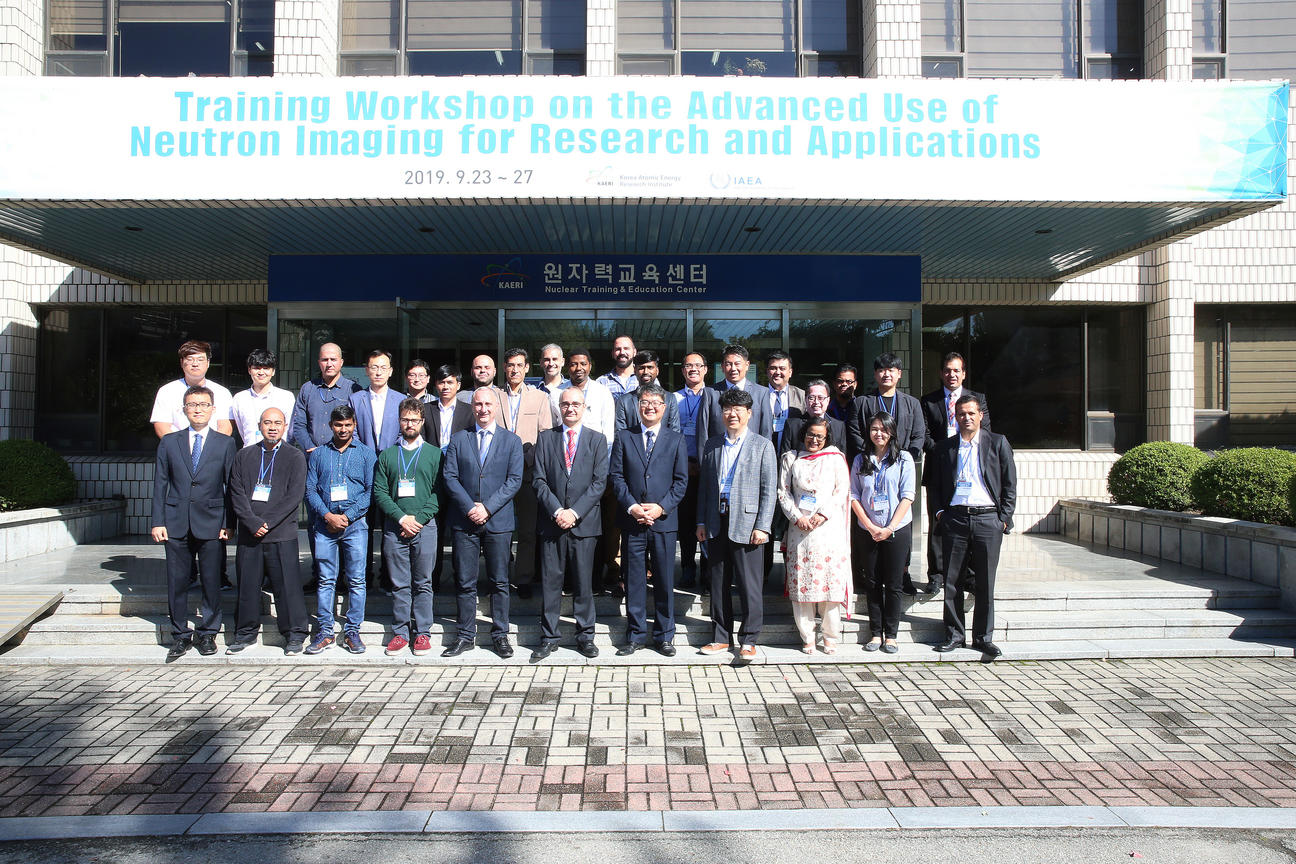
\includegraphics[scale=0.25]{figures/grupo.jpg}
    \end{center}
\end{frame}

%-------------------------------------------------
\begin{frame}
  \frametitle{AUNIRA 2019 - Daejeon, República da Coréia}
  \framesubtitle{Advanced Use of Neutron Imaging for Research and Applications}
  \begin{itemize}
  \item 2019: foco em aplicações de  Herança Cultural
  \item Anfitriões: KAERI (Korea Atomic Energy Research Institute)
  \item 21 participantes de 18 países
  \item Duração de uma semana (segunda até meio-dia de sexta-feira)
  \end{itemize}
  Formato:
  \begin{itemize}
  \item Apresentações
  \item Visita técnica às instalações do reator HANARO
  \item Uma seção prática: uso do software \textit{VG Studio}\textcopyright
  \item Seção de posters
  \end{itemize}

\end{frame}

%-------------------------------------------------
\begin{frame}
  \frametitle{AUNIRA 2019 - Daejeon, República da Coréia}
  \framesubtitle{Advanced Use of Neutron Imaging for Research and Applications}
  \begin{center}
    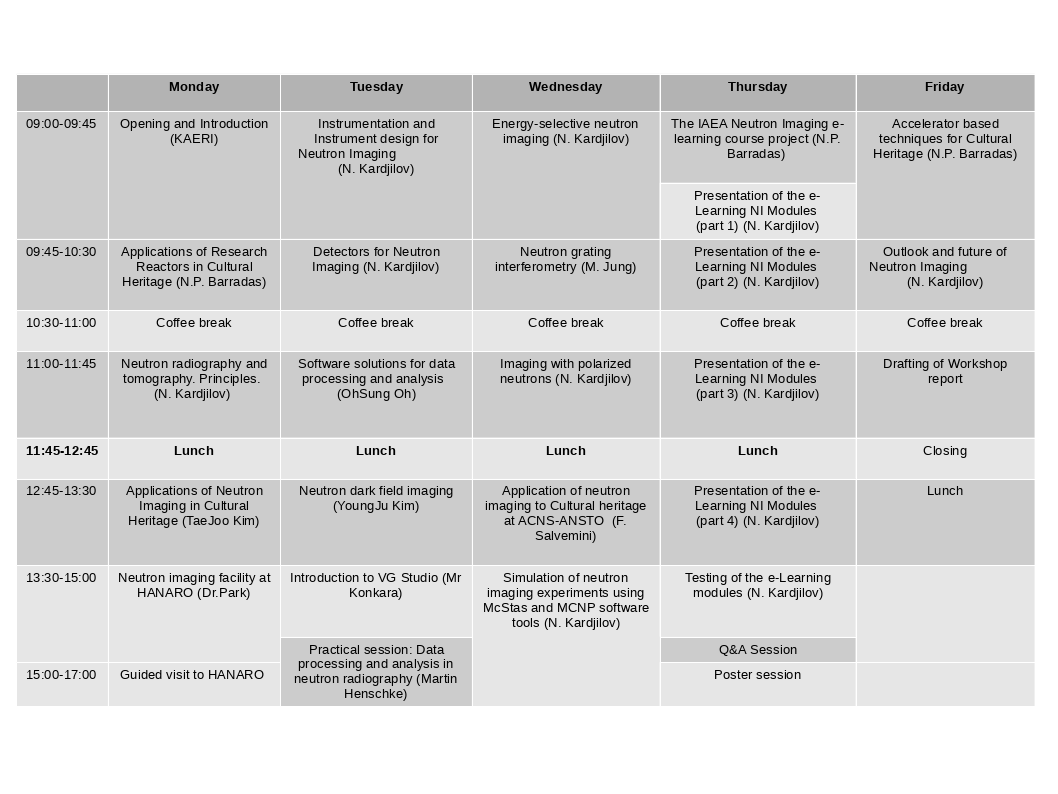
\includegraphics[scale=2.0]{figures/agenda.png}
    \end{center}
\end{frame}

%-------------------------------------------------
\begin{frame}
  \frametitle{AUNIRA 2019 - Daejeon, República da Coréia}
  \framesubtitle{Advanced Use of Neutron Imaging for Research and Applications}
  \begin{center}
    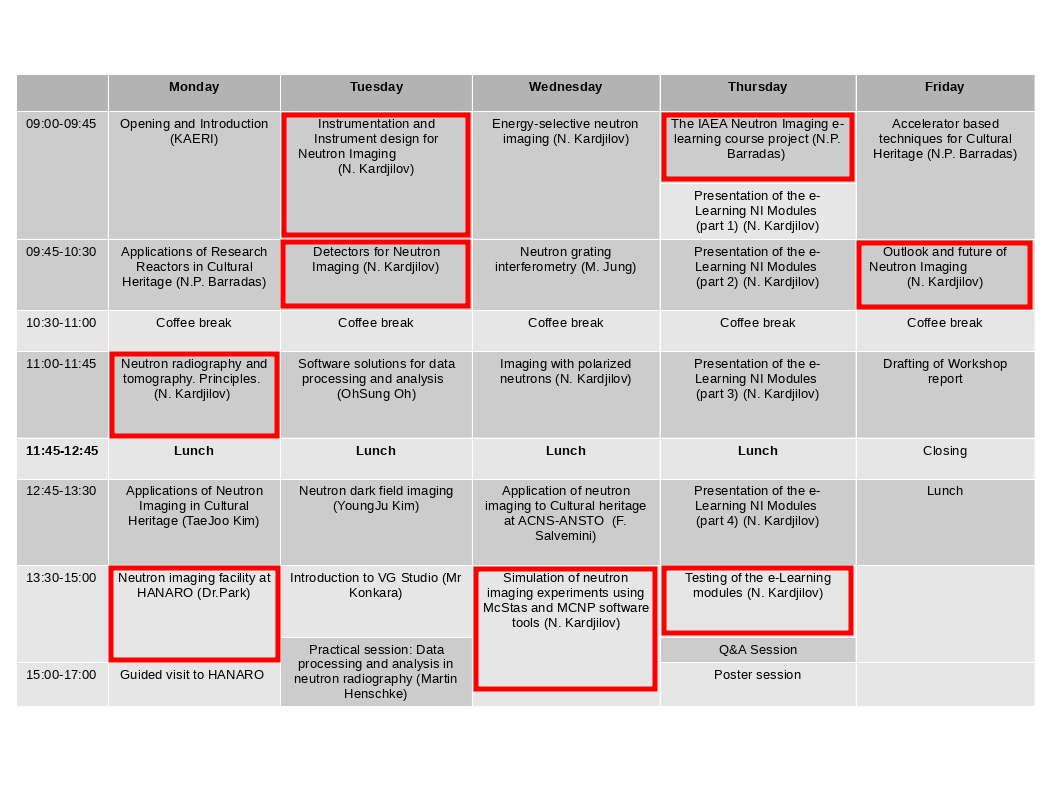
\includegraphics[scale=2.0]{figures/agenda-marked.png}
    \end{center}
\end{frame}

%-------------------------------------------------


\section{Apresentações escolhidas}
%-------------------------------------------------
\subsection{Neutron Radiography and Tomography: Principles}
%-------------------------------------------------
\begin{frame}
  \frametitle{Apresentações escolhidas}
  \framesubtitle{(1)}
  \begin{center}
    Neutron Radiography and Tomography: Principles\\
    \vspace{2.0cm}
    N. Kardjilov
  \end{center}
\end{frame}

\begin{frame}
  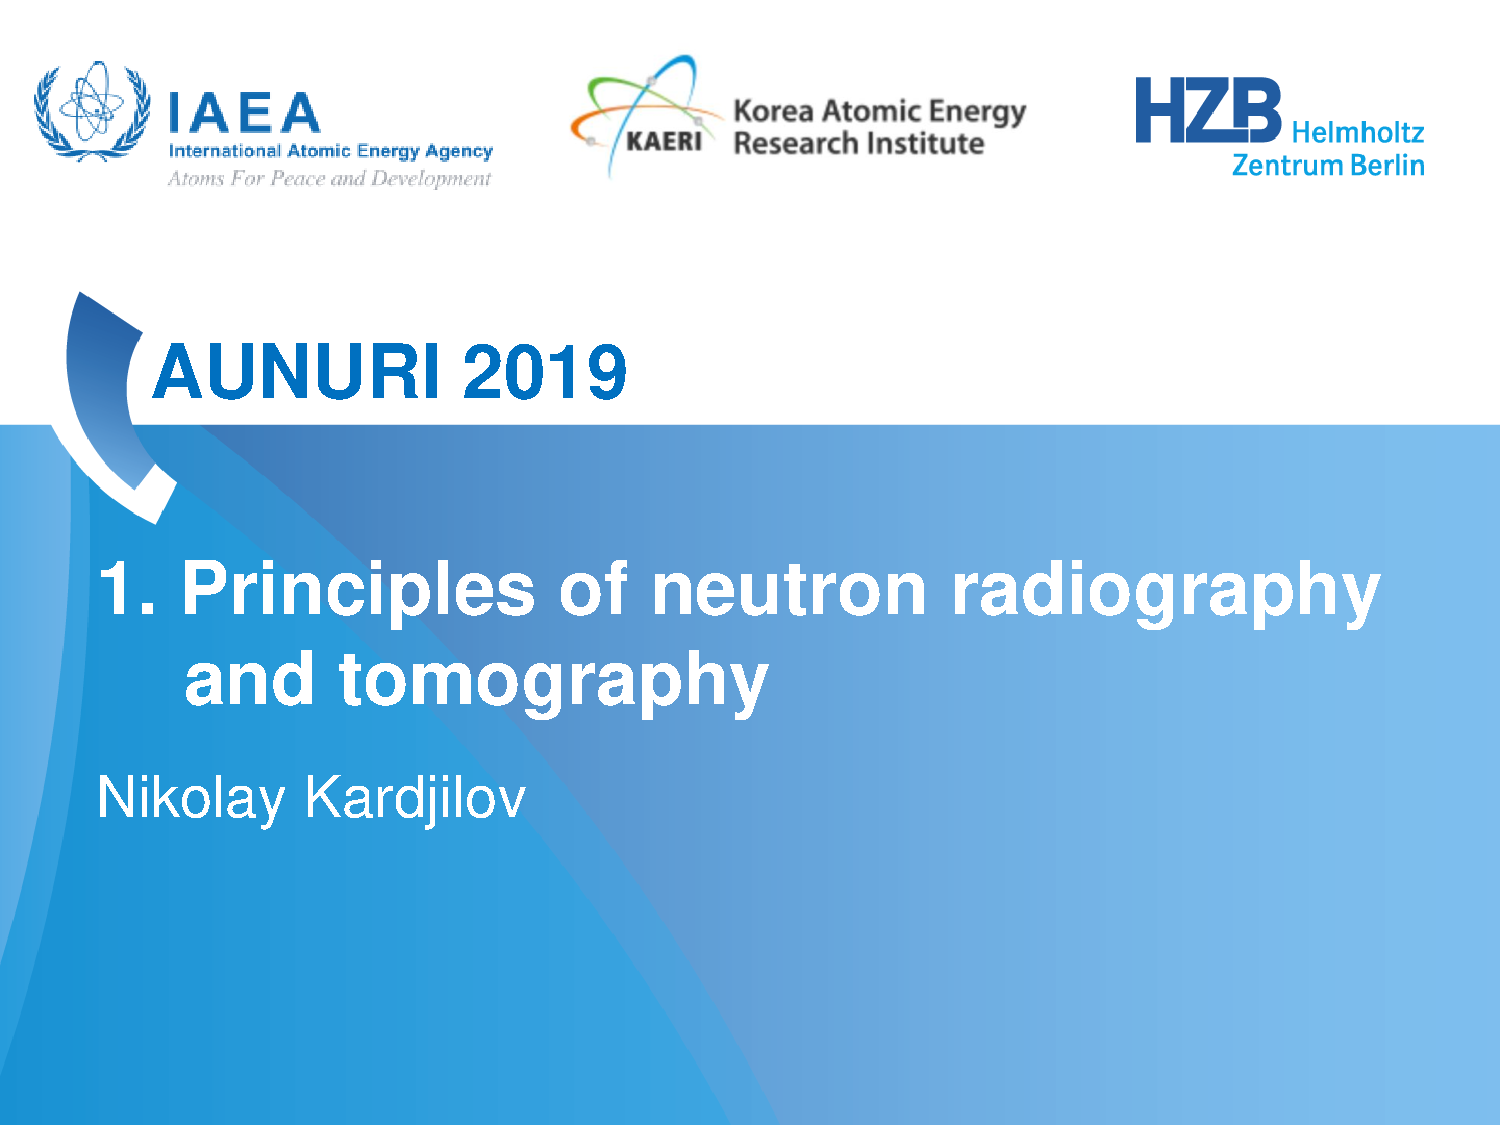
\includepdf{figures/pres1/sl1.pdf}
\end{frame}

\begin{frame}
  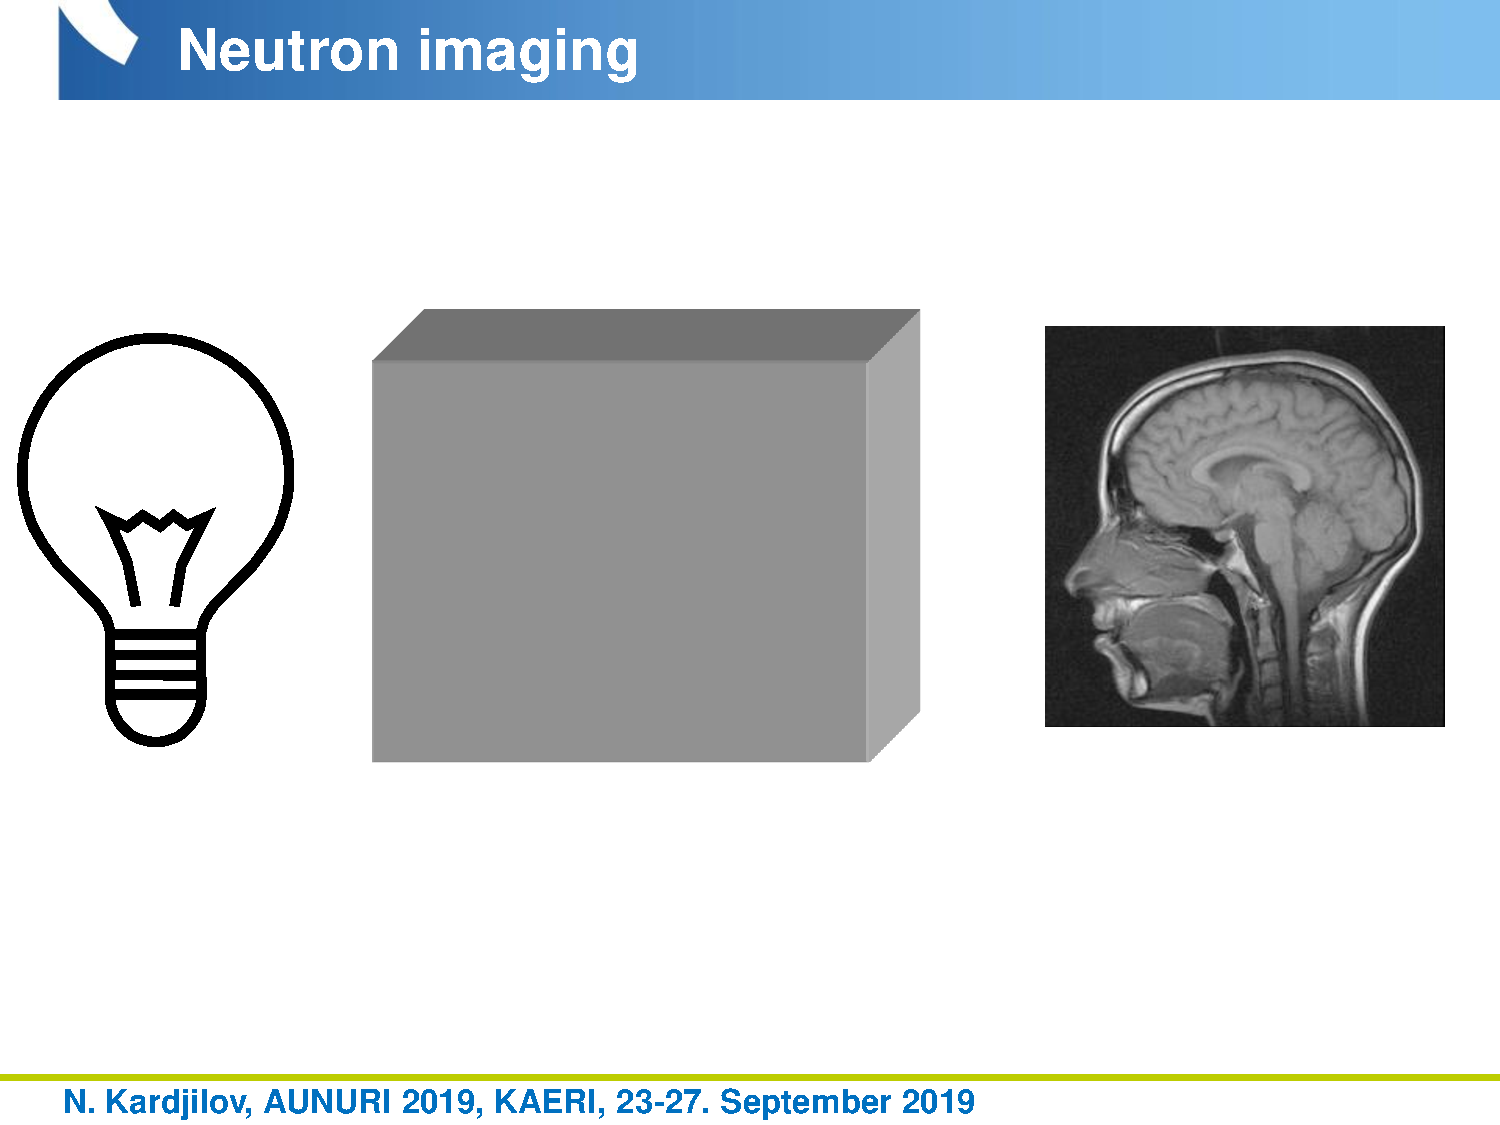
\includepdf{figures/pres1/sl5.pdf}
\end{frame}

\begin{frame}
    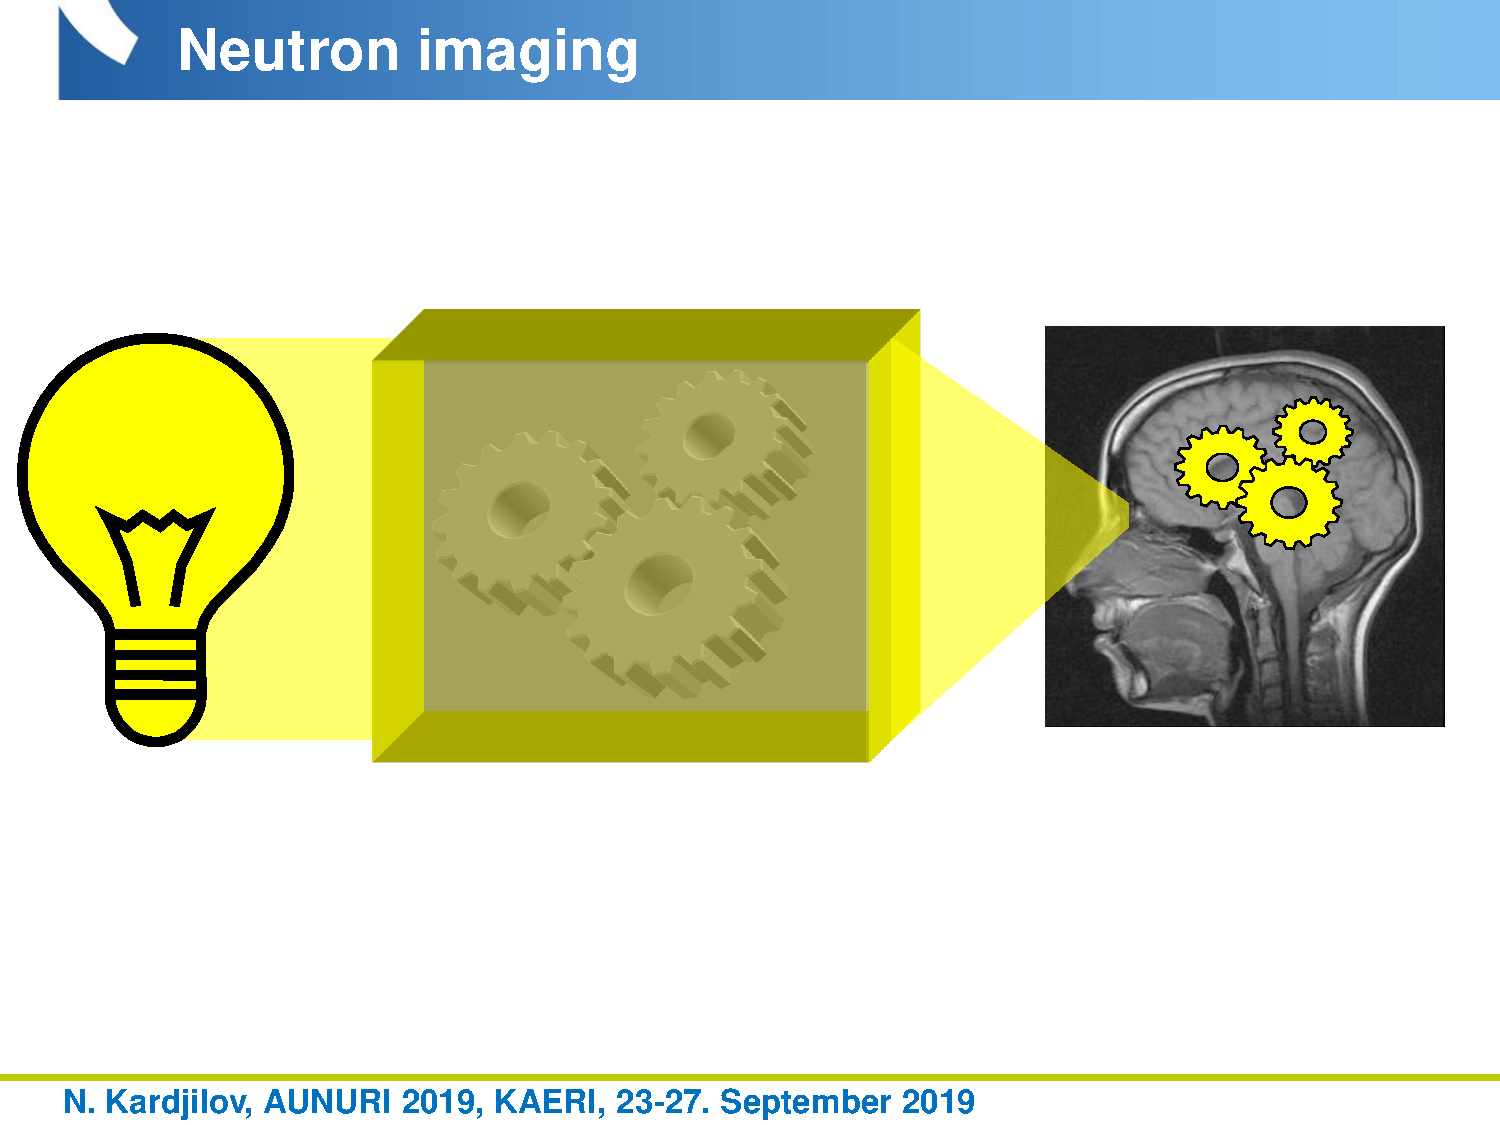
\includepdf{figures/pres1/sl6.pdf}
\end{frame}

\begin{frame}
  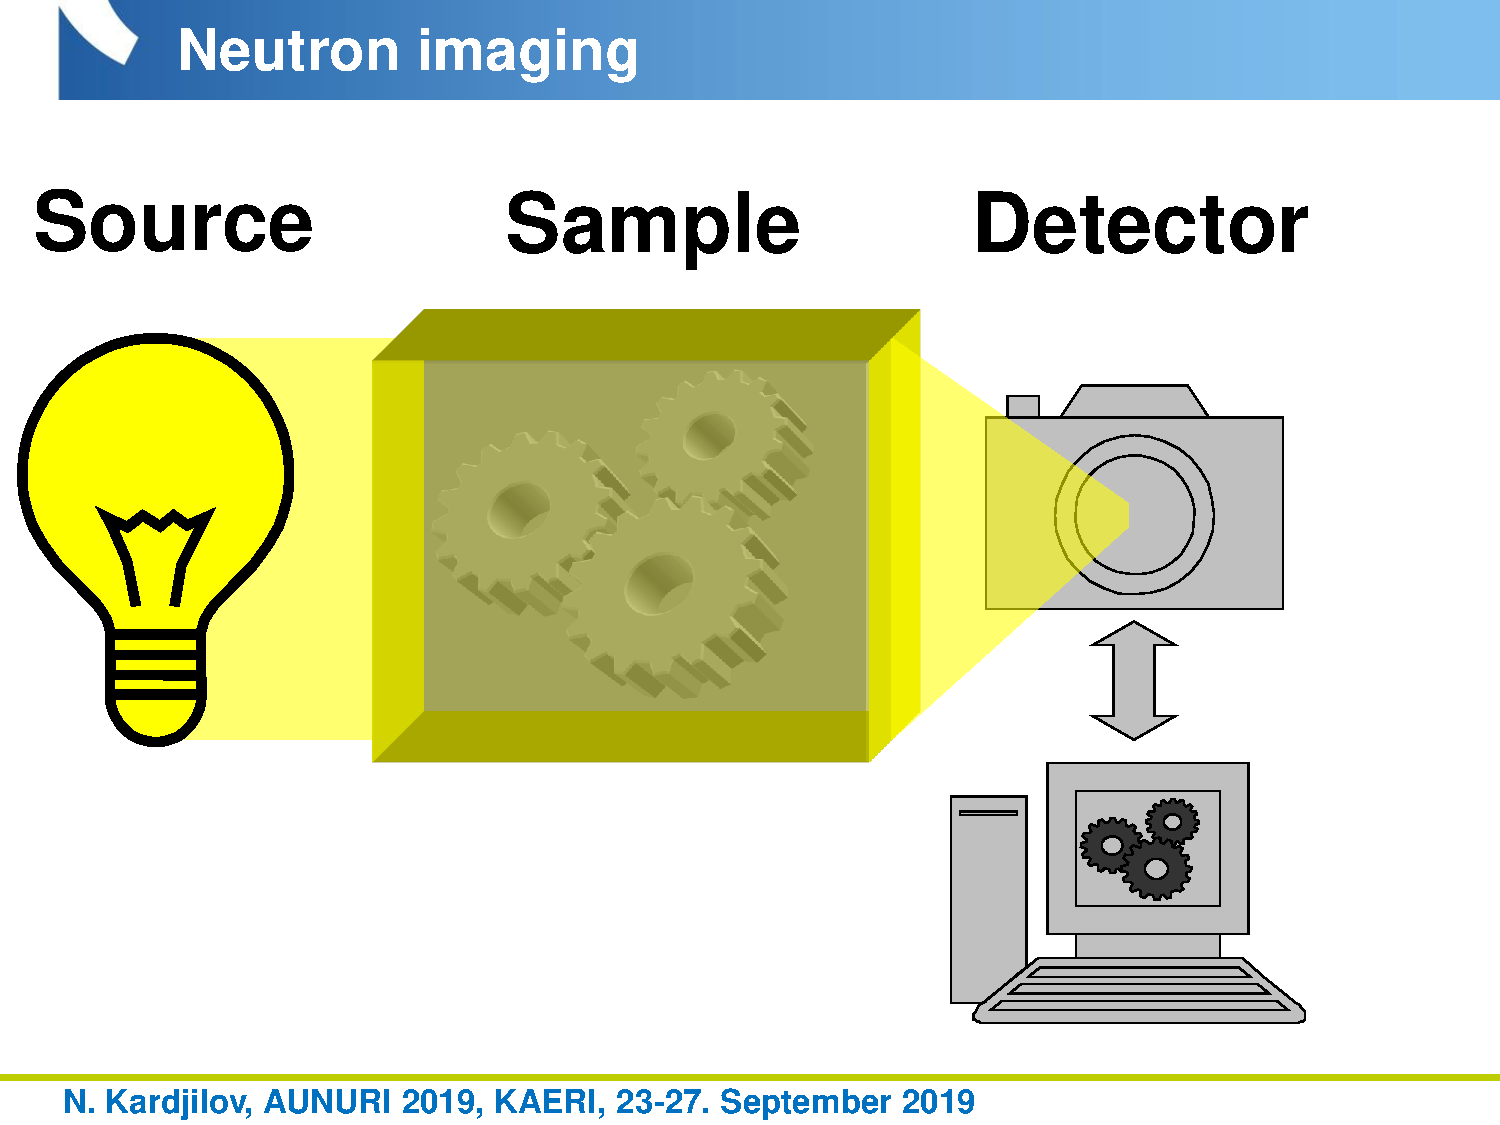
\includepdf{figures/pres1/sl7.pdf}
\end{frame}

\begin{frame}
  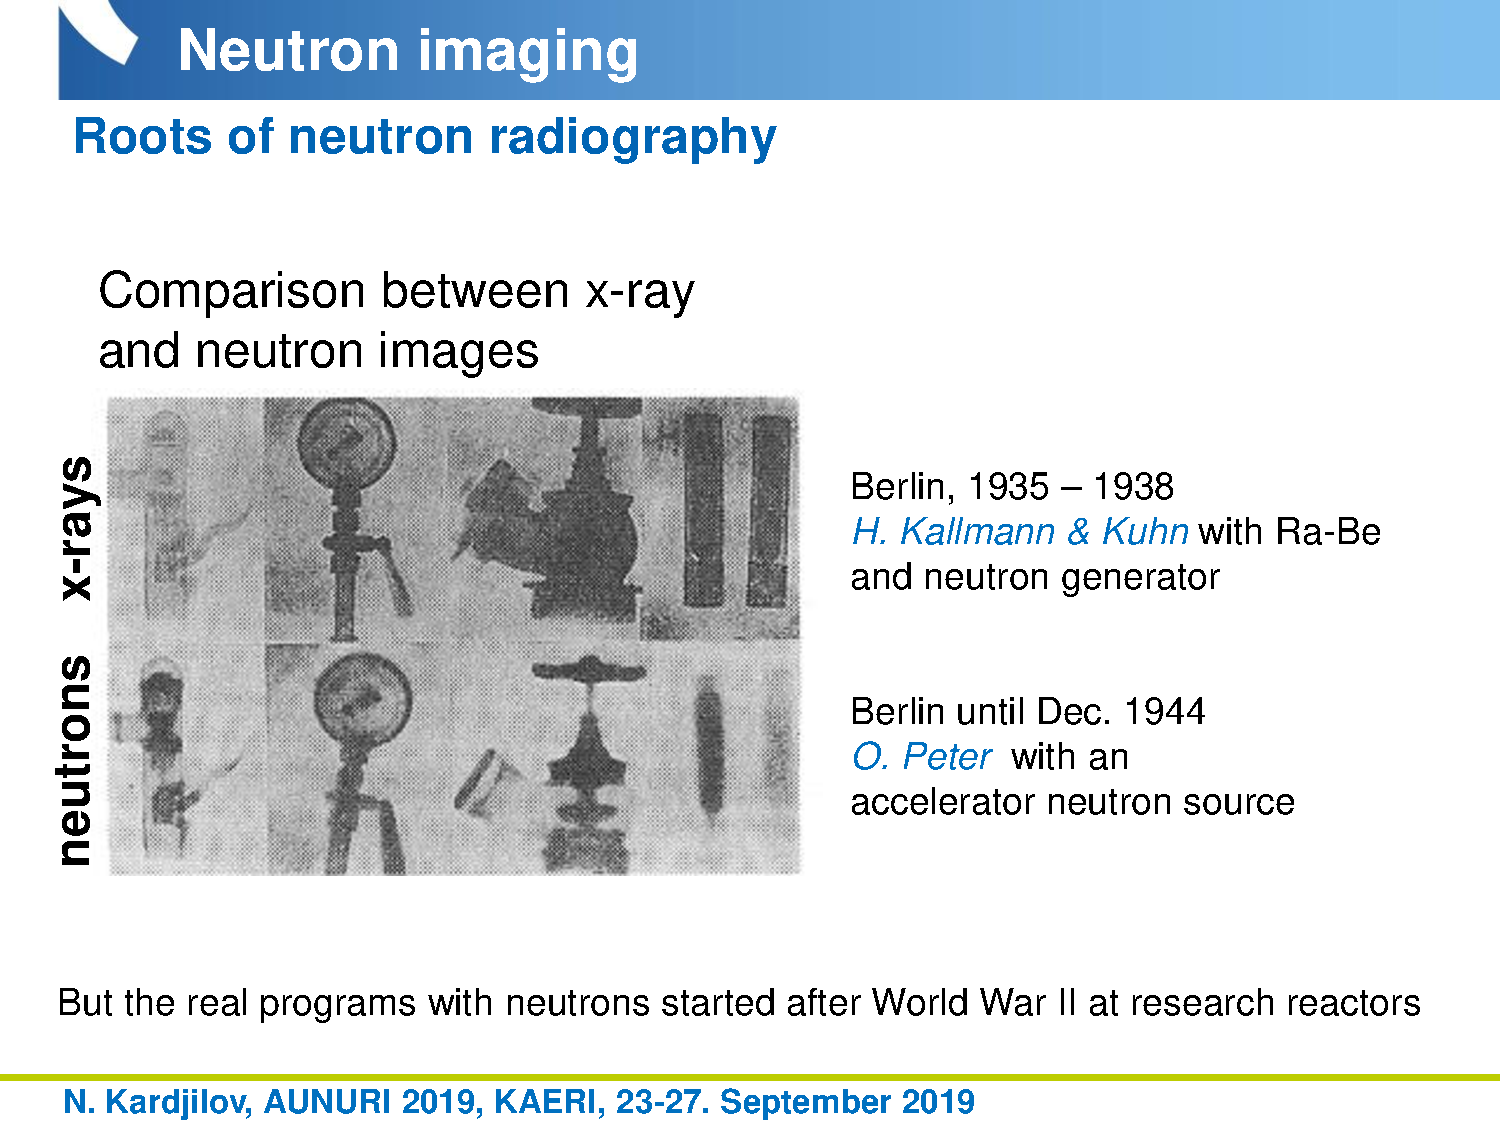
\includepdf{figures/pres1/sl10.pdf}
\end{frame}

\begin{frame}
  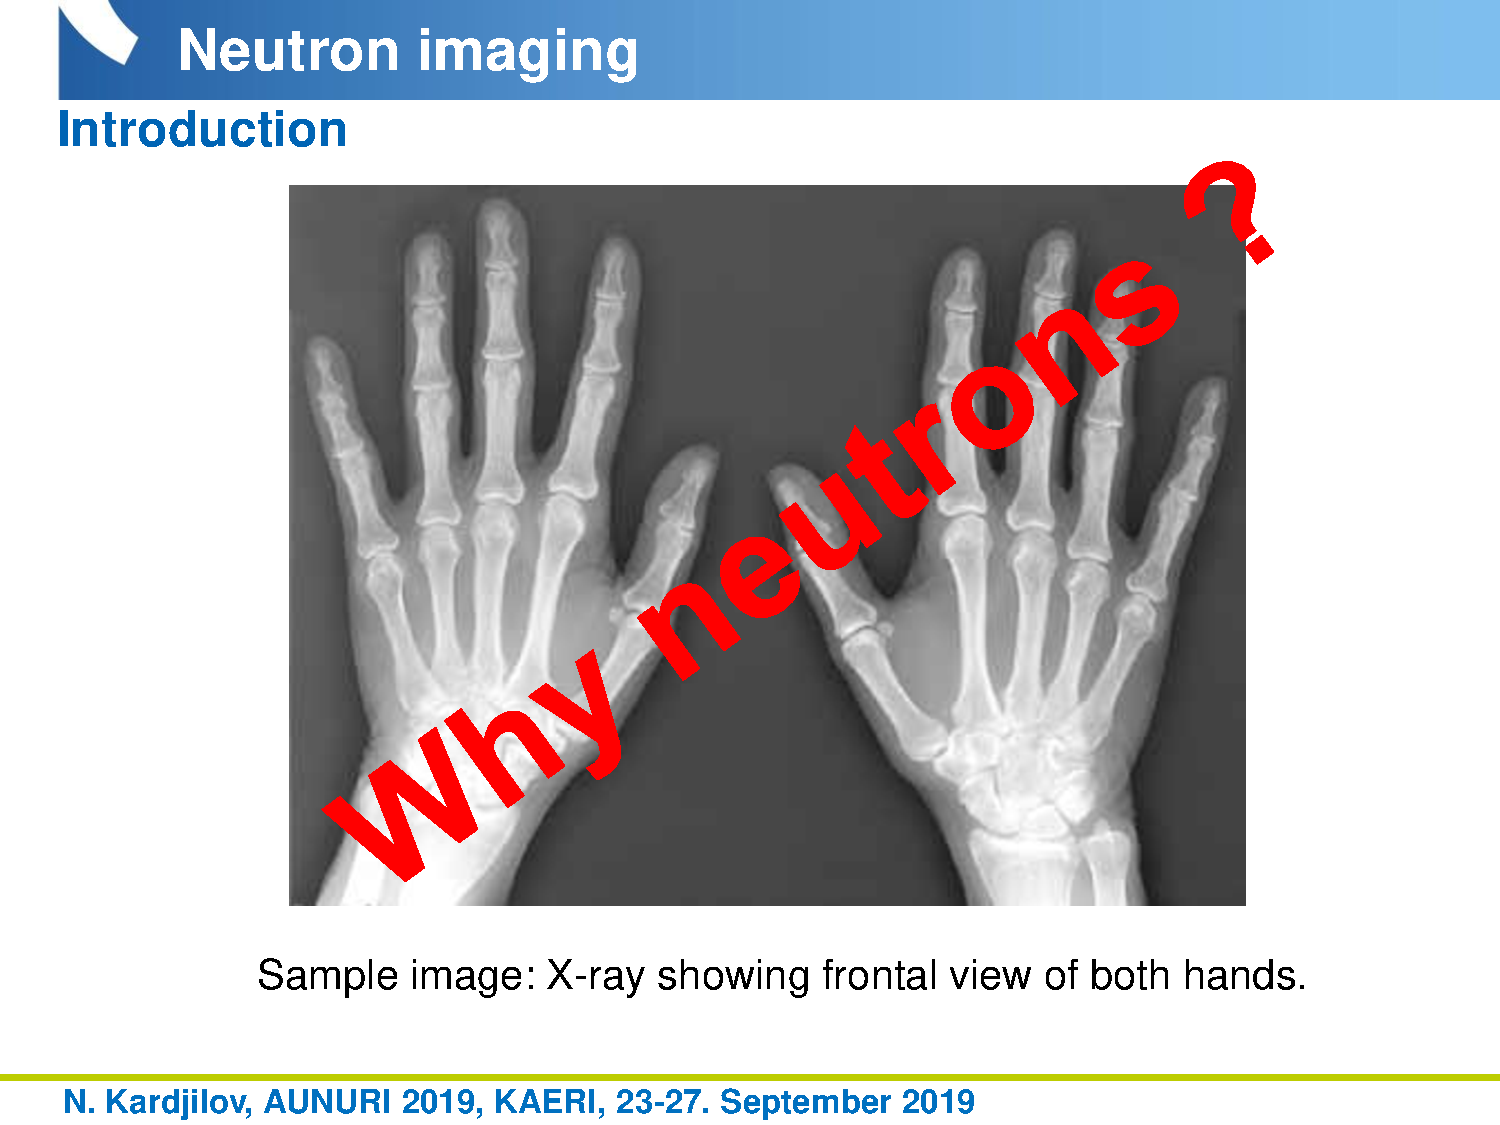
\includepdf{figures/pres1/sl11.pdf}
\end{frame}

\begin{frame}
  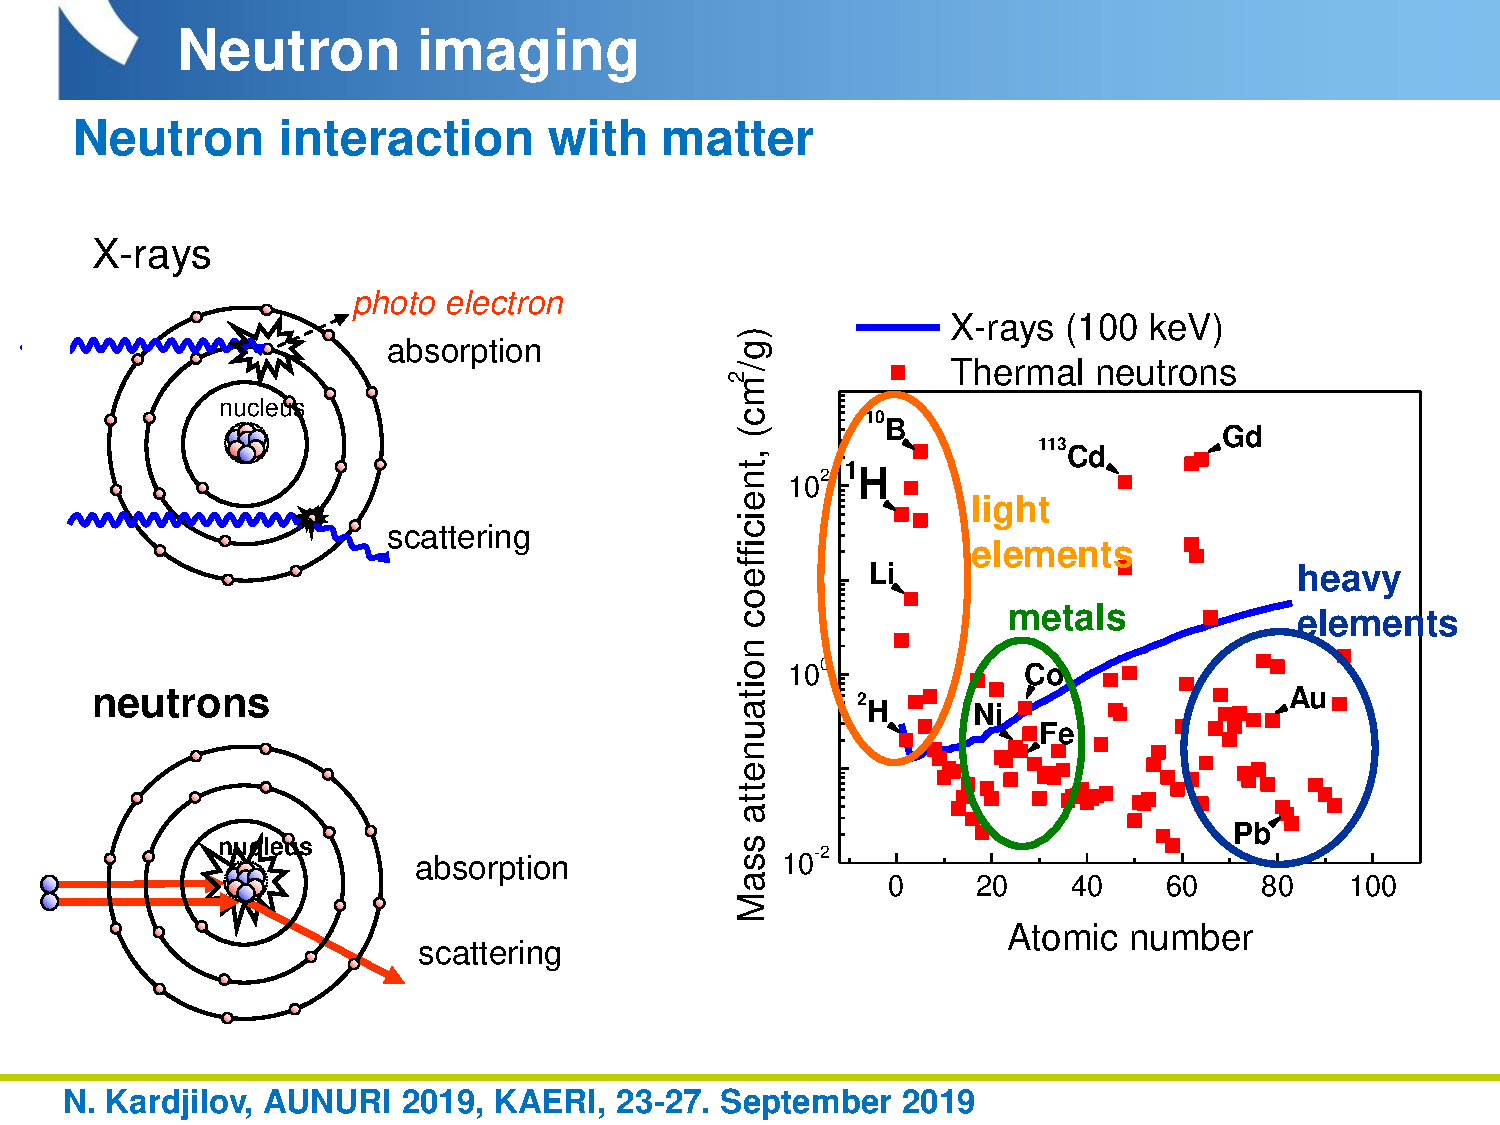
\includepdf{figures/pres1/sl12.pdf}
\end{frame}

\begin{frame}
  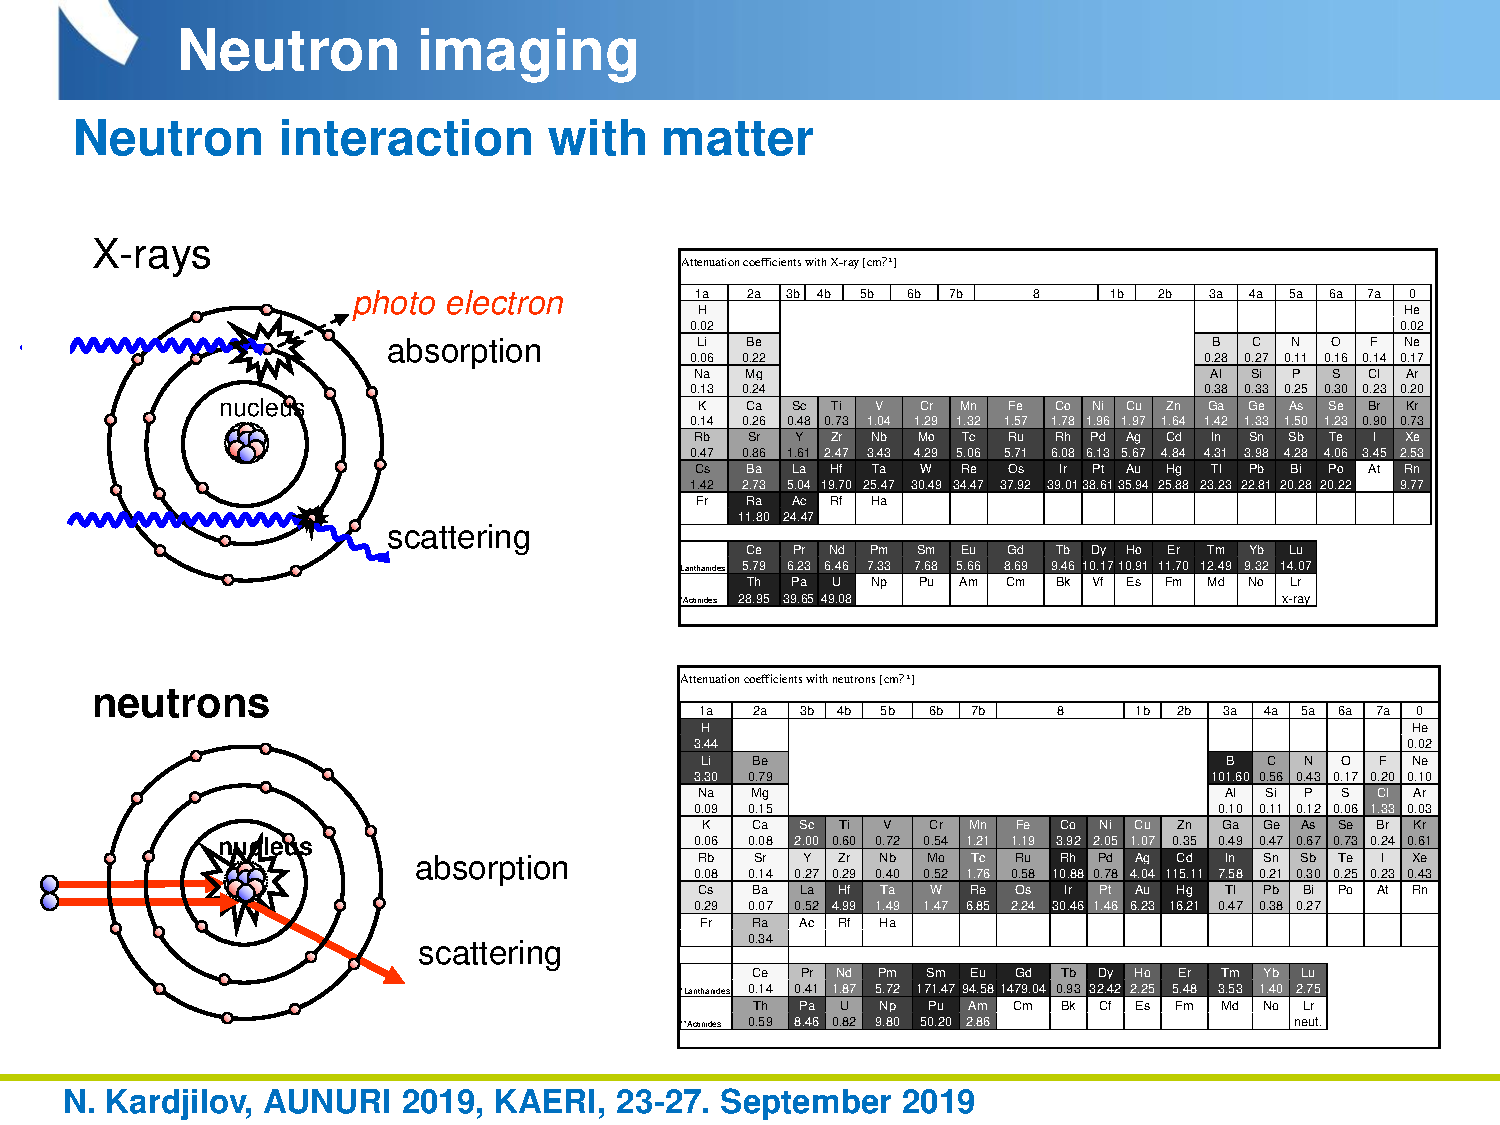
\includepdf{figures/pres1/sl13.pdf}
\end{frame}

\begin{frame}
  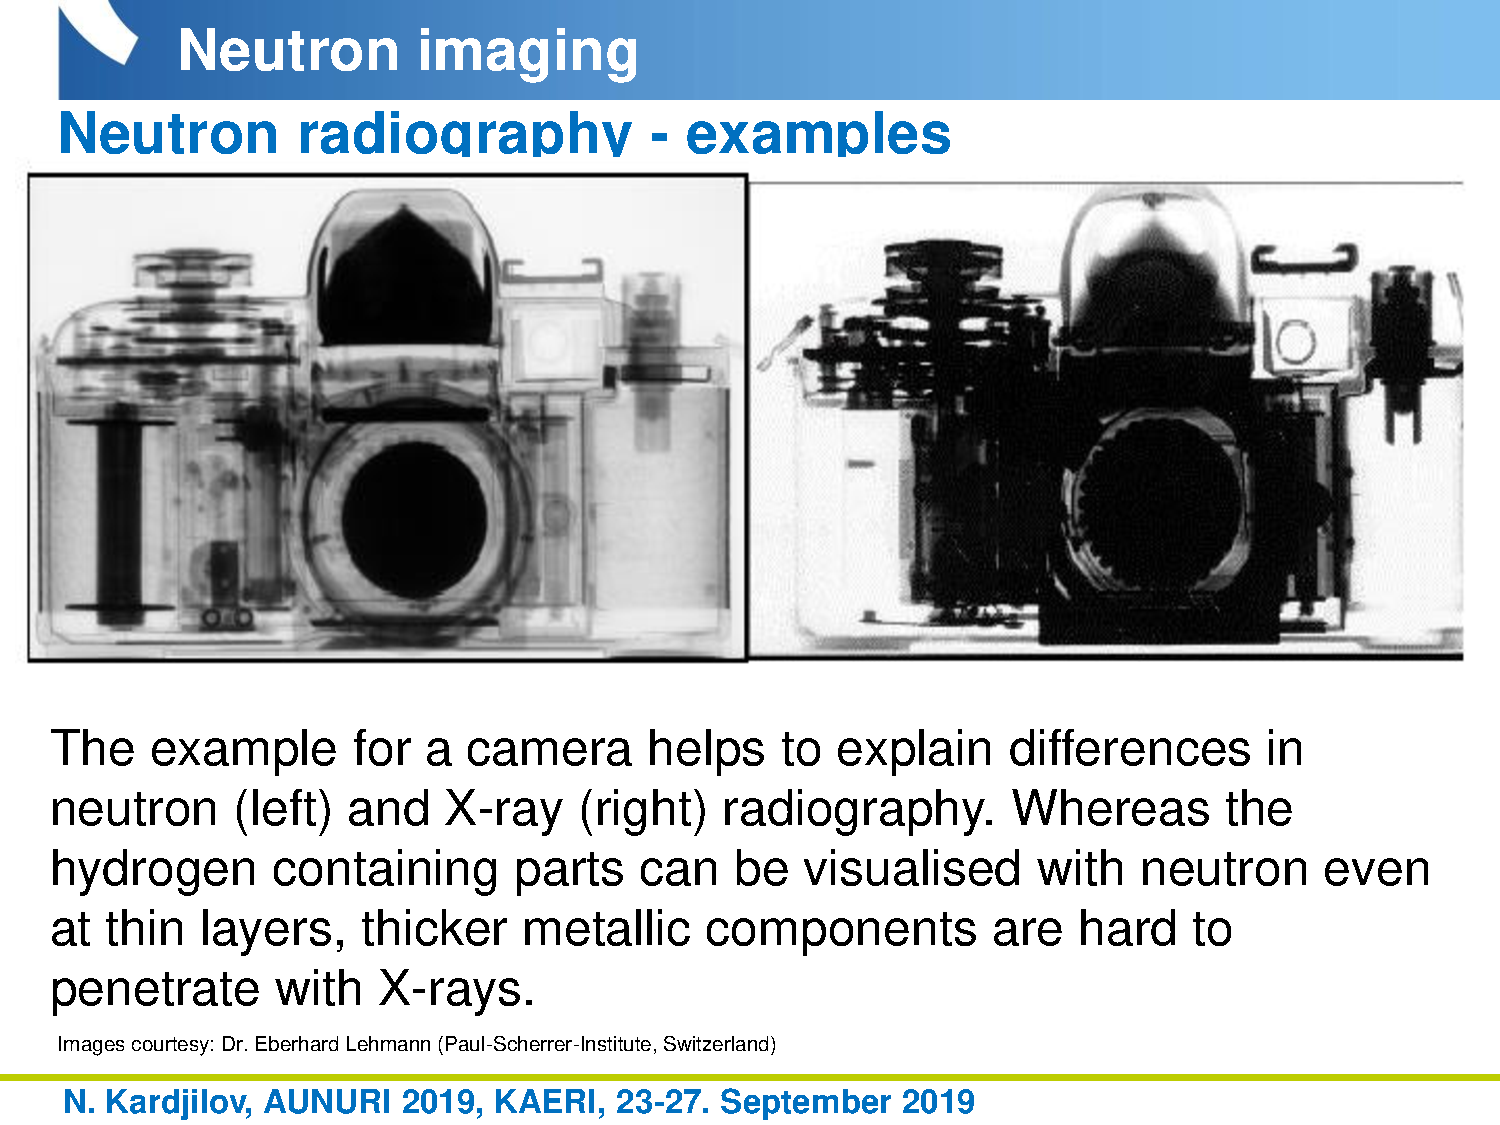
\includepdf{figures/pres1/sl14.pdf}
\end{frame}

%-------------------------------------------------
\subsection{Neutron Imaging Facility at HANARO}
%-------------------------------------------------
\begin{frame}
  \frametitle{Apresentações escolhidas}
  \framesubtitle{(2)}
  \begin{center}
    Neutron Imaging Facility at HANARO\\
    \vspace{2.0cm}
    Dr. Park
  \end{center}
\end{frame}


\begin{frame}
  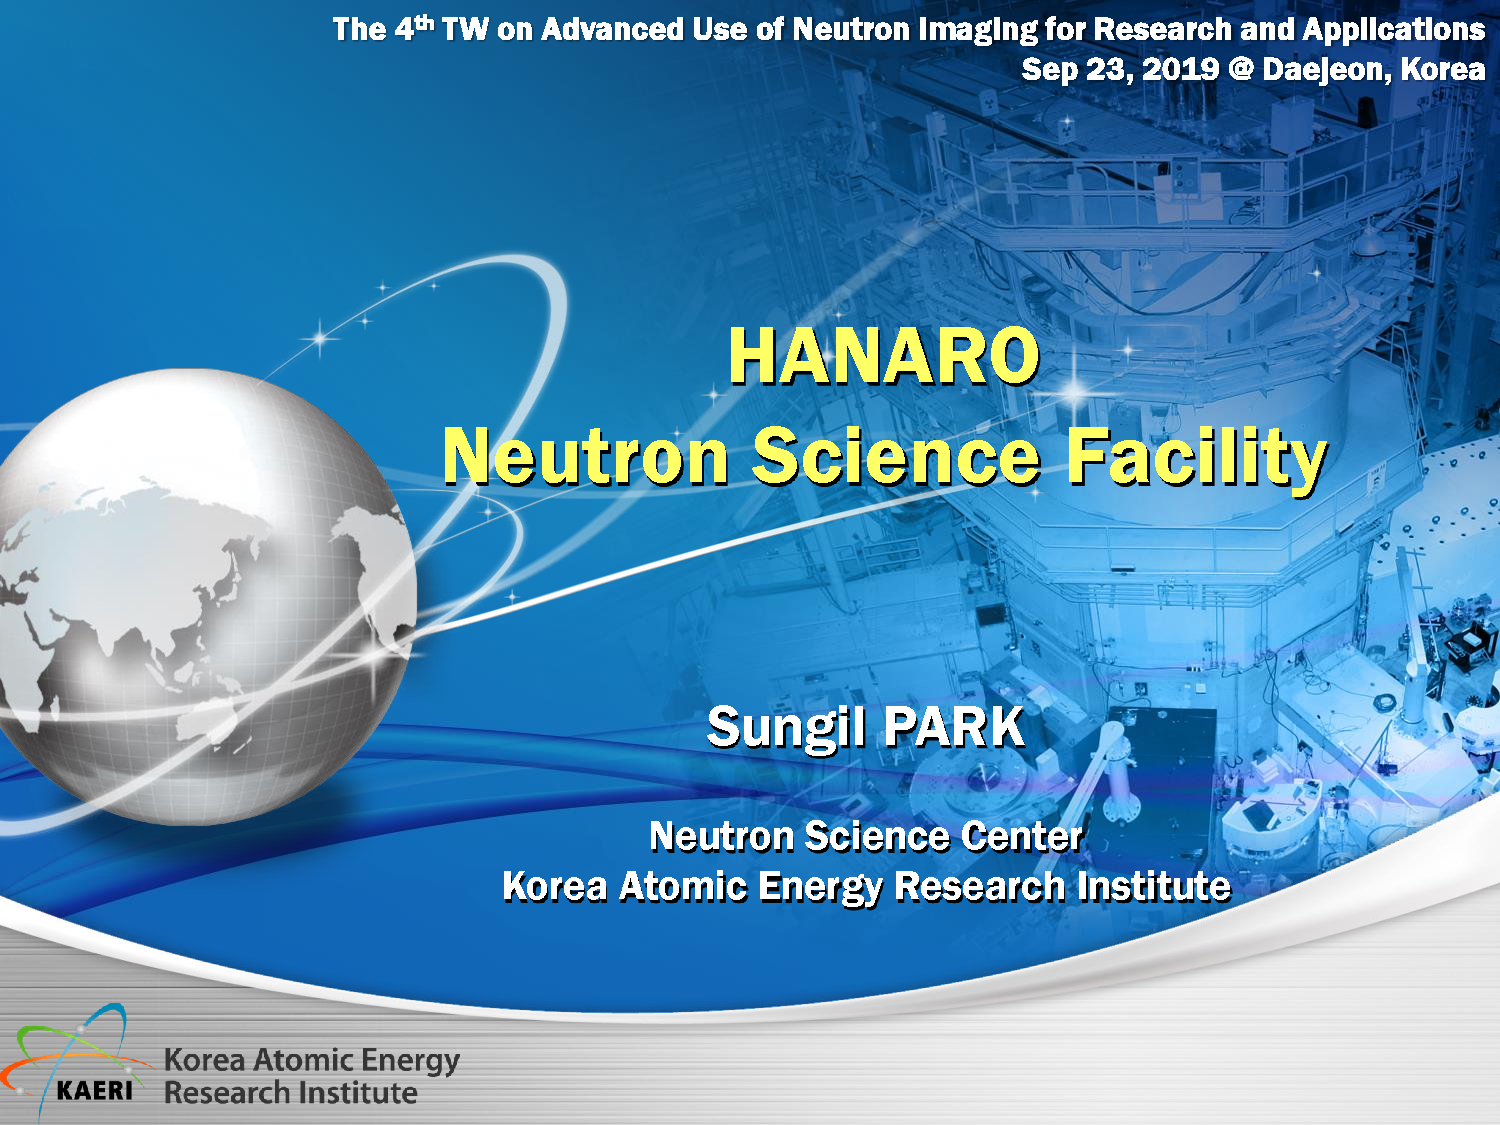
\includepdf{figures/pres2/sl-1.pdf}
\end{frame}

\begin{frame}
  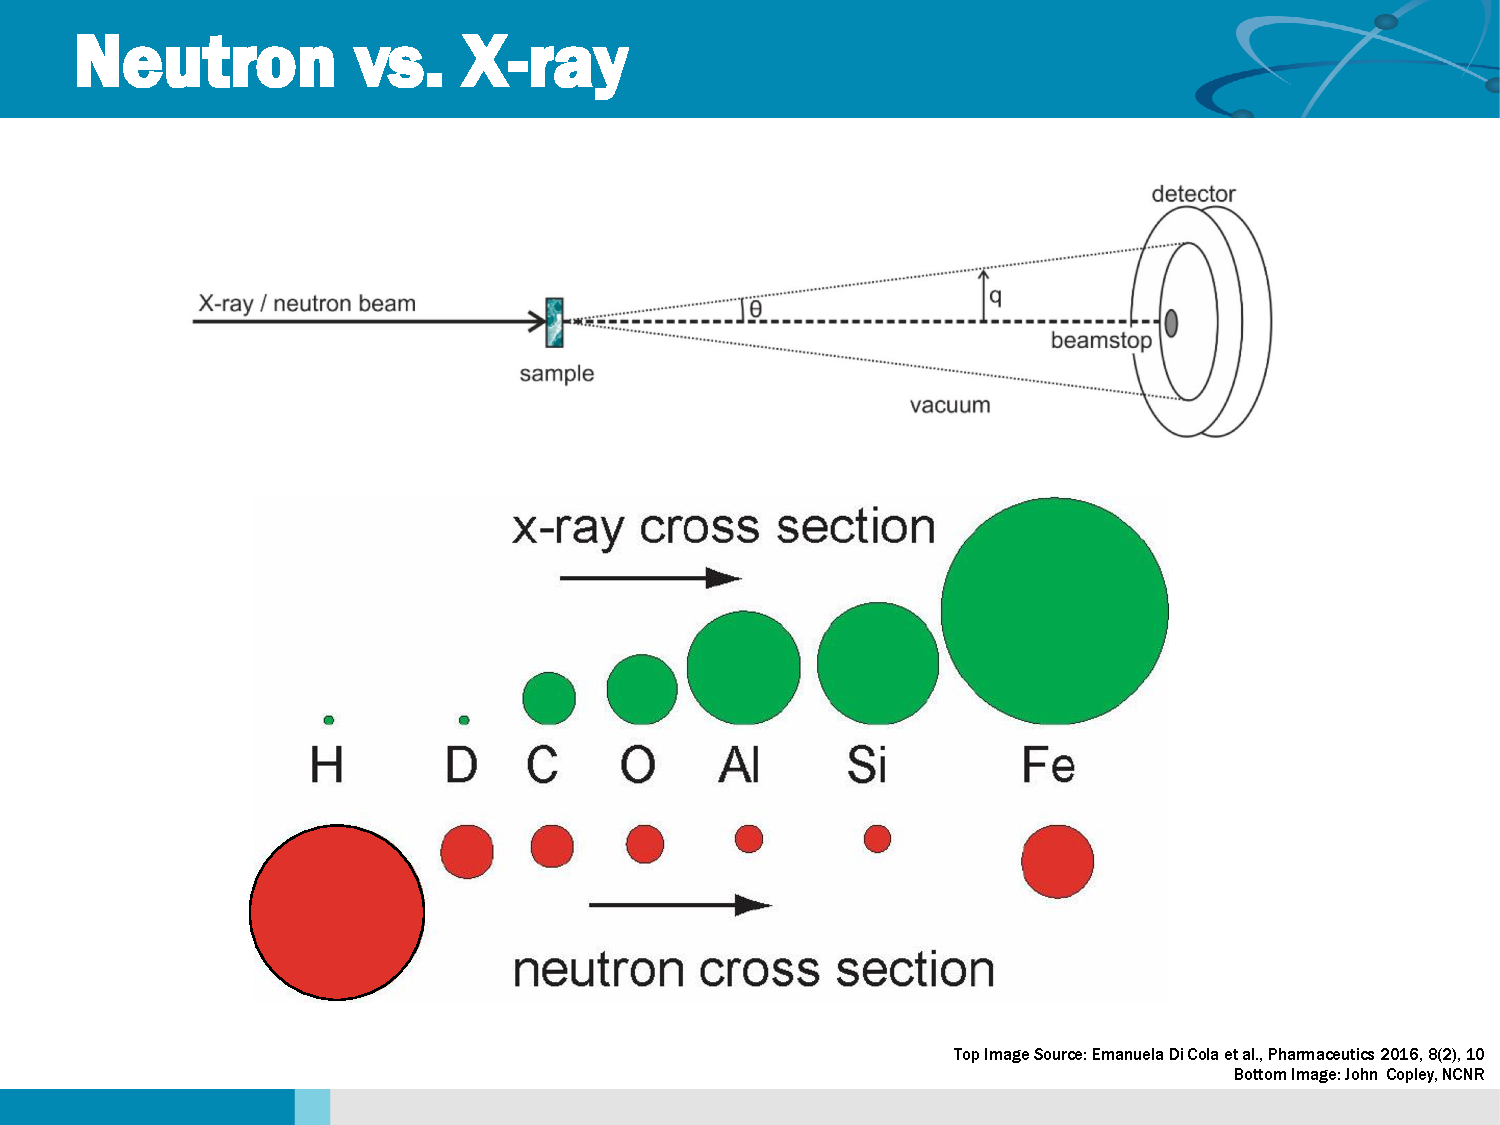
\includepdf{figures/pres2/sl-3.pdf}
\end{frame}

\begin{frame}
    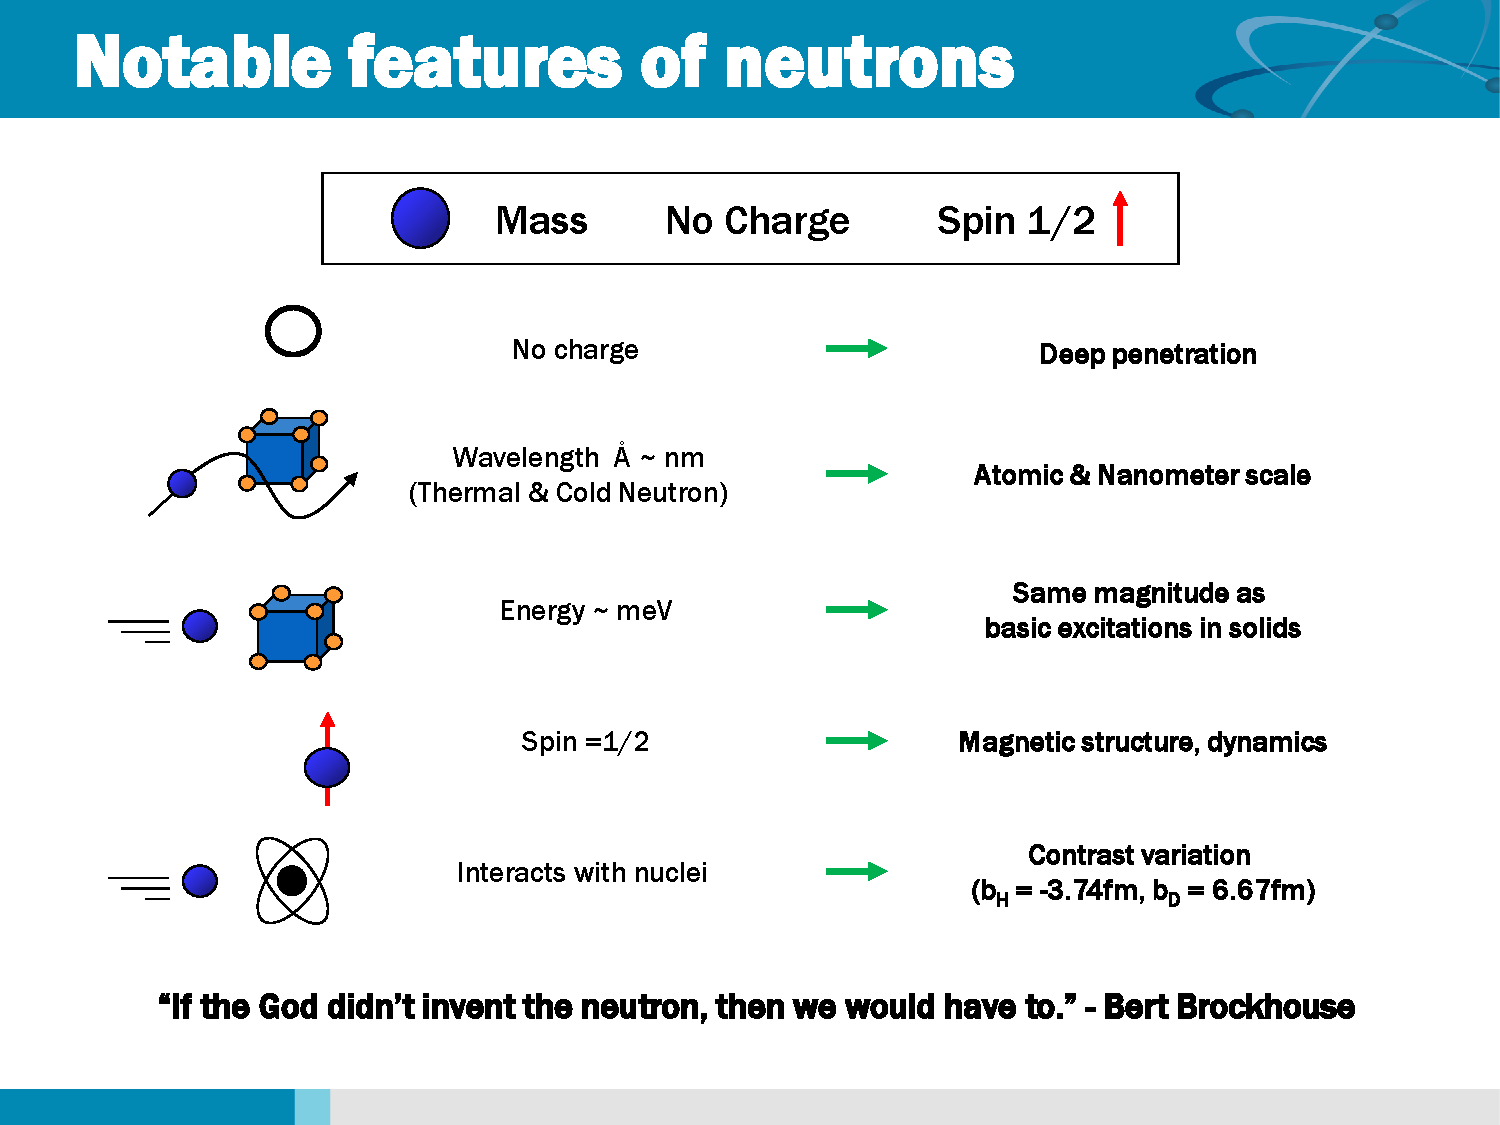
\includepdf{figures/pres2/sl-4.pdf}
\end{frame}

\begin{frame}
  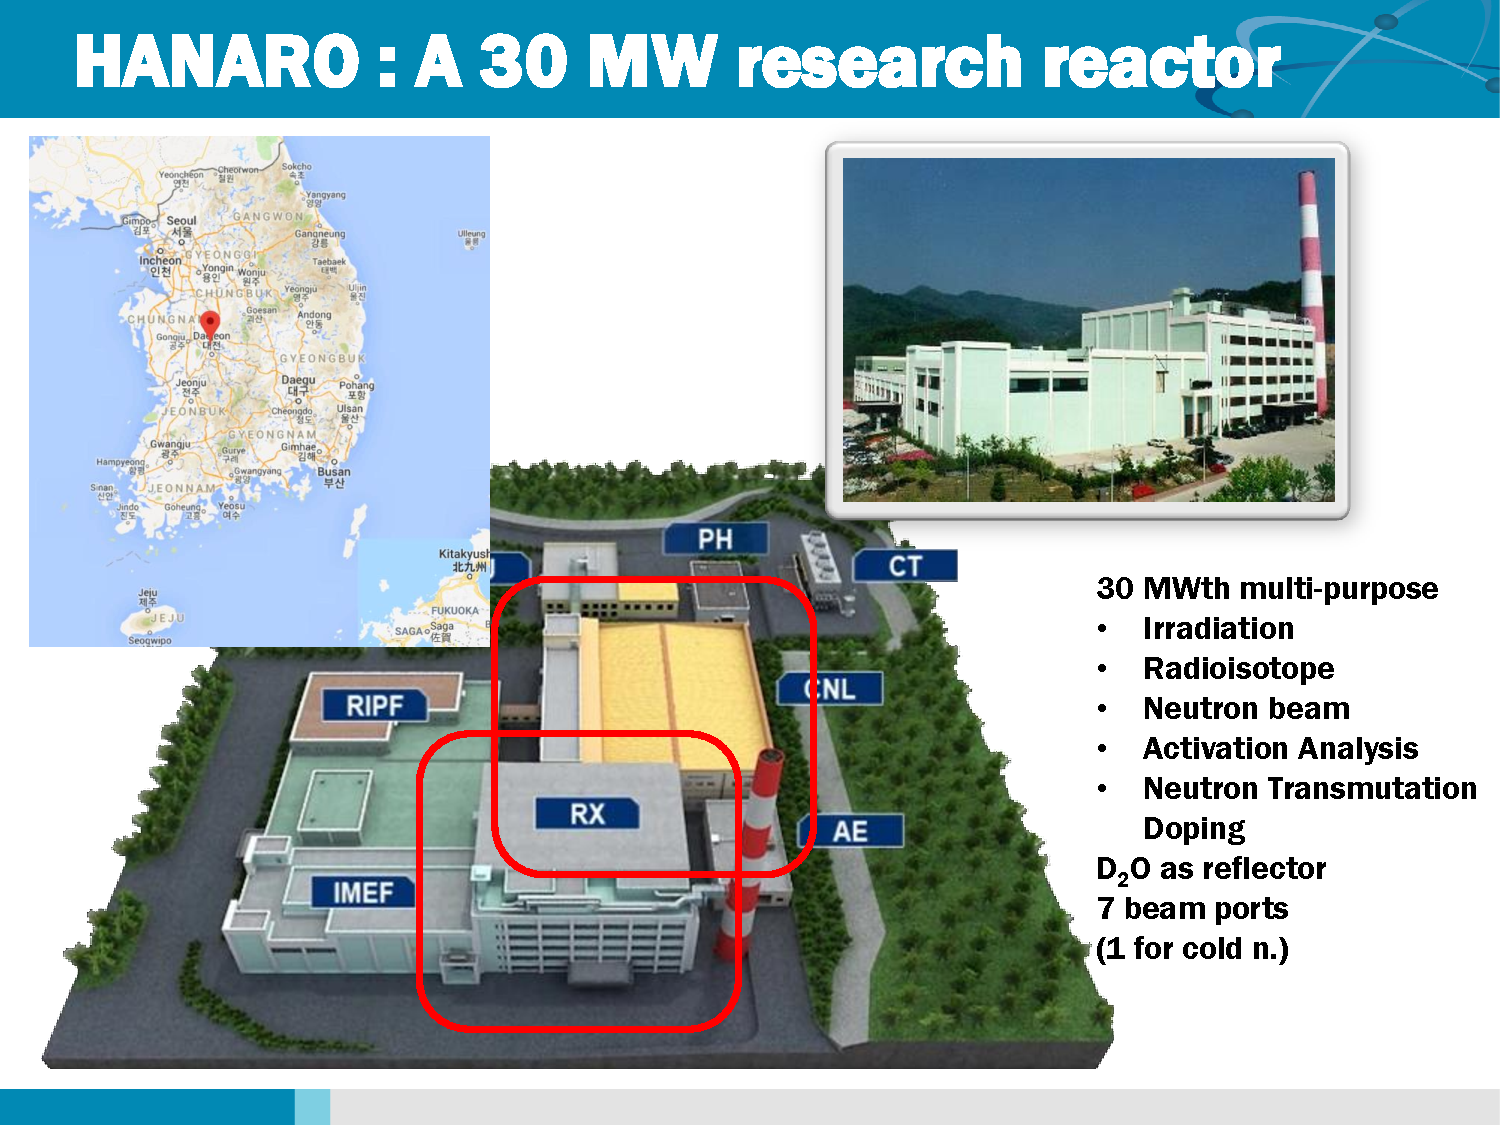
\includepdf{figures/pres2/sl-10.pdf}
\end{frame}

\begin{frame}
  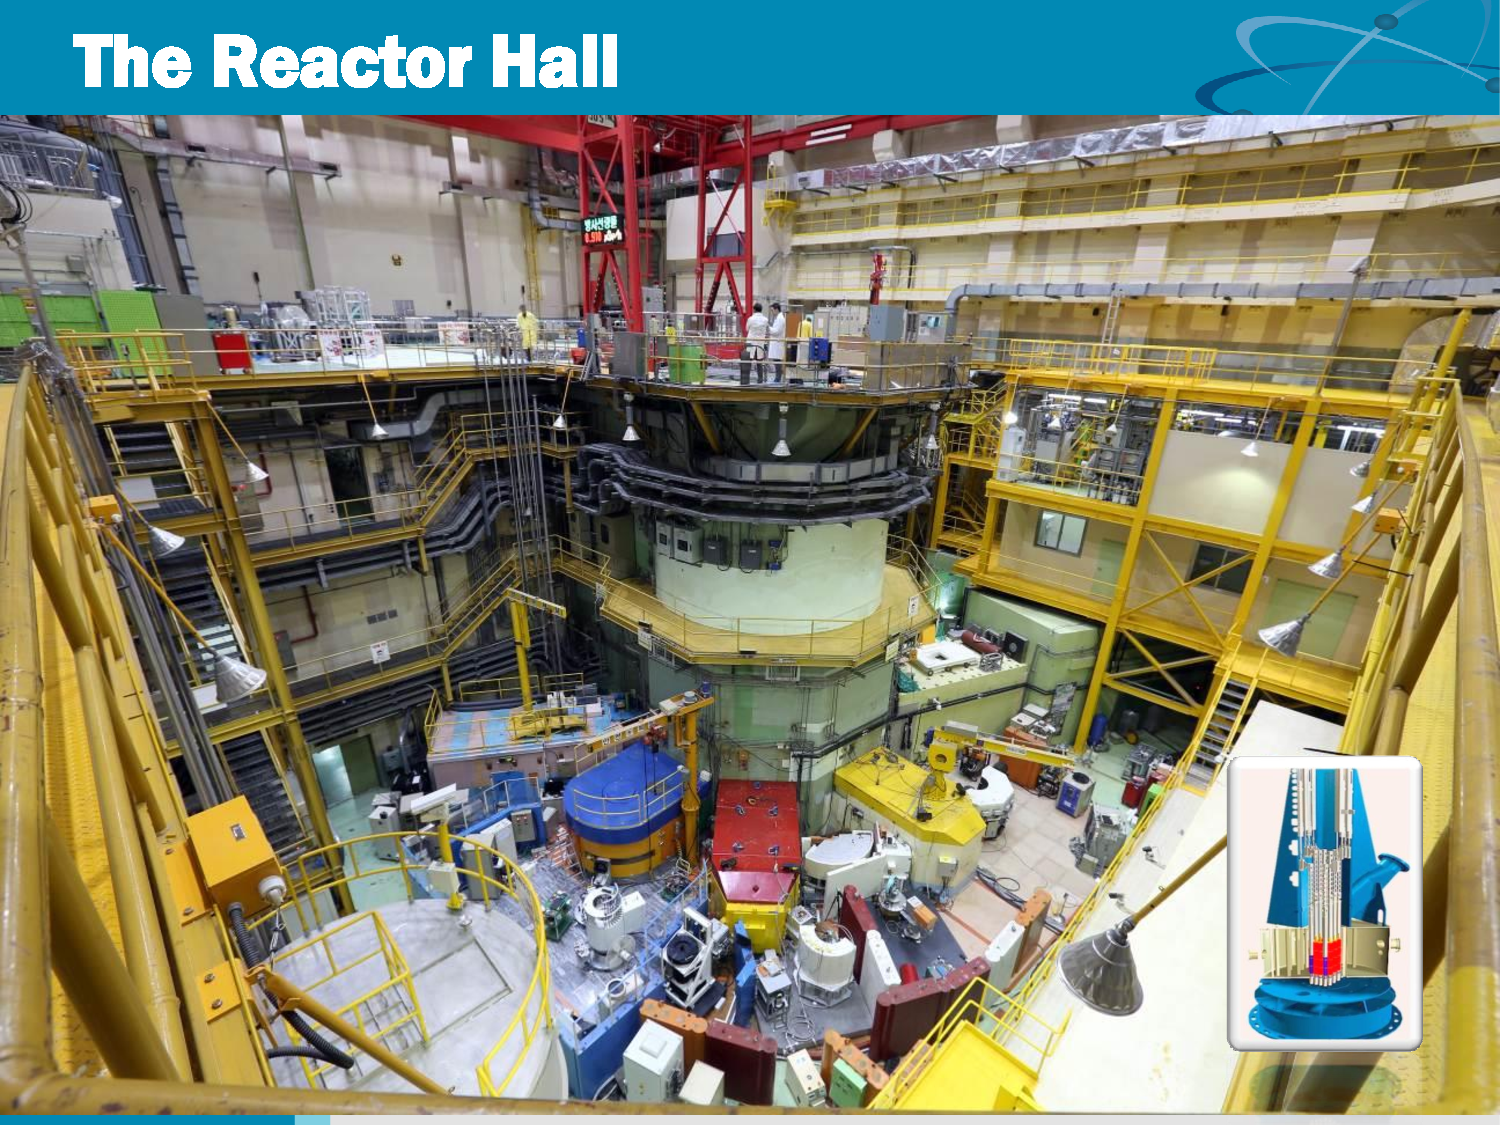
\includepdf{figures/pres2/sl-11.pdf}
\end{frame}

\begin{frame}
  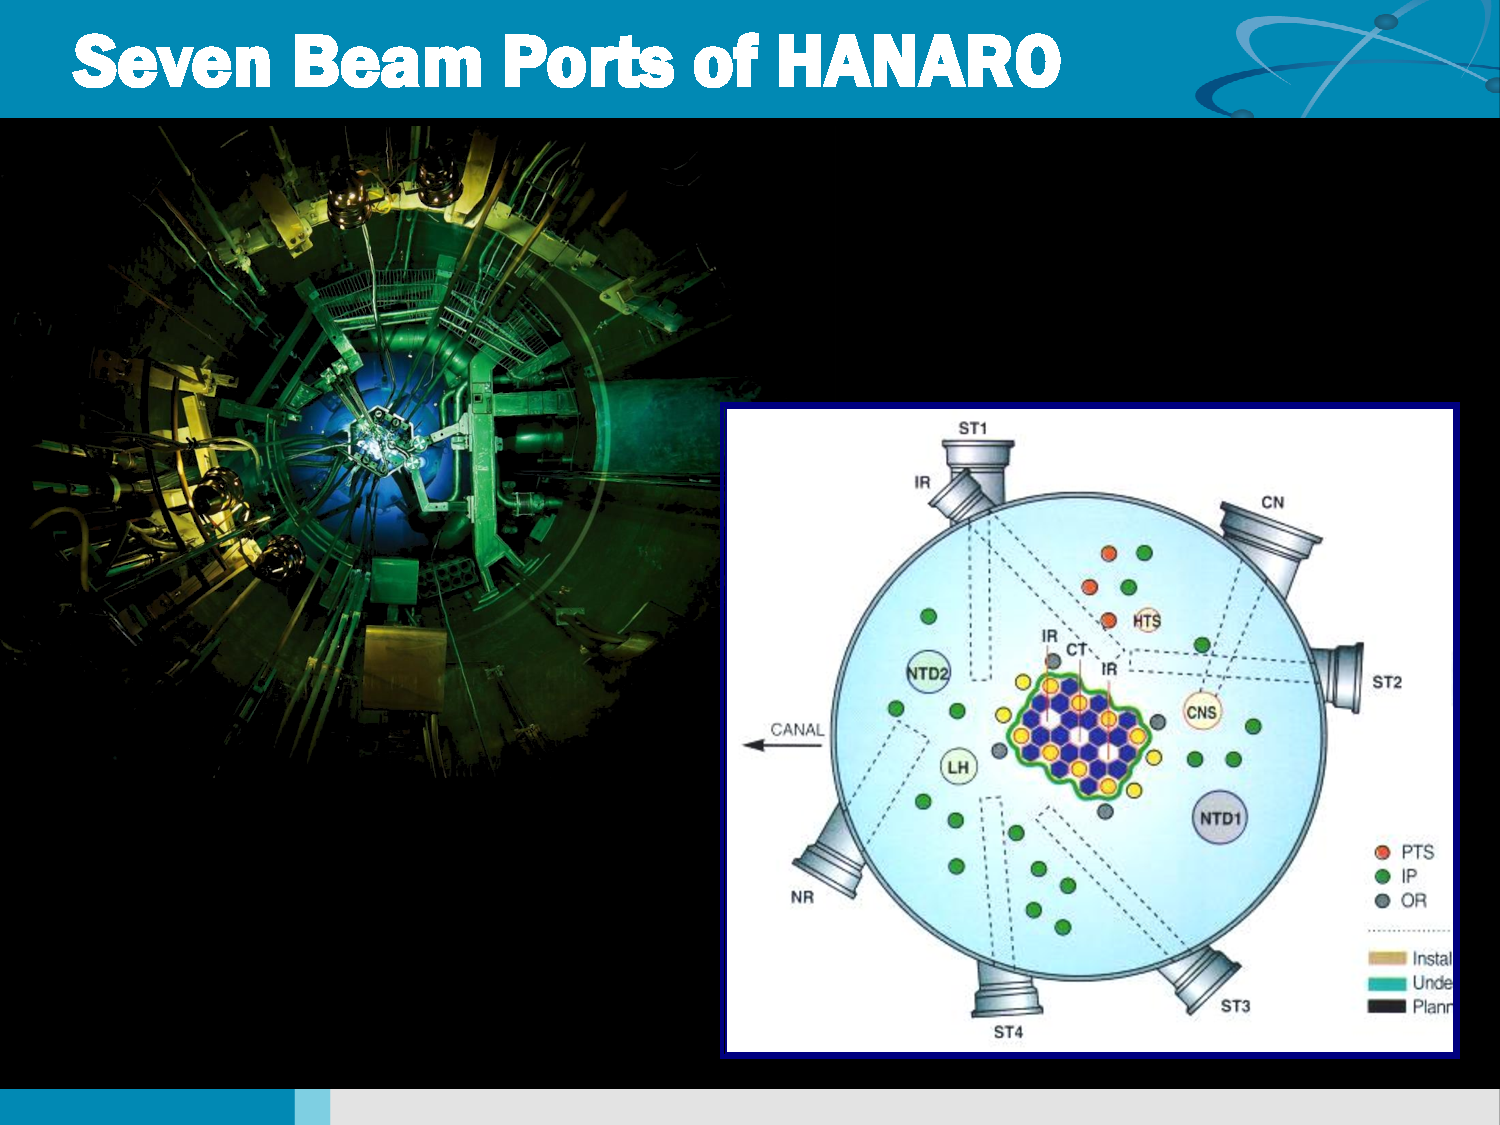
\includepdf{figures/pres2/sl-12.pdf}
\end{frame}

\begin{frame}
  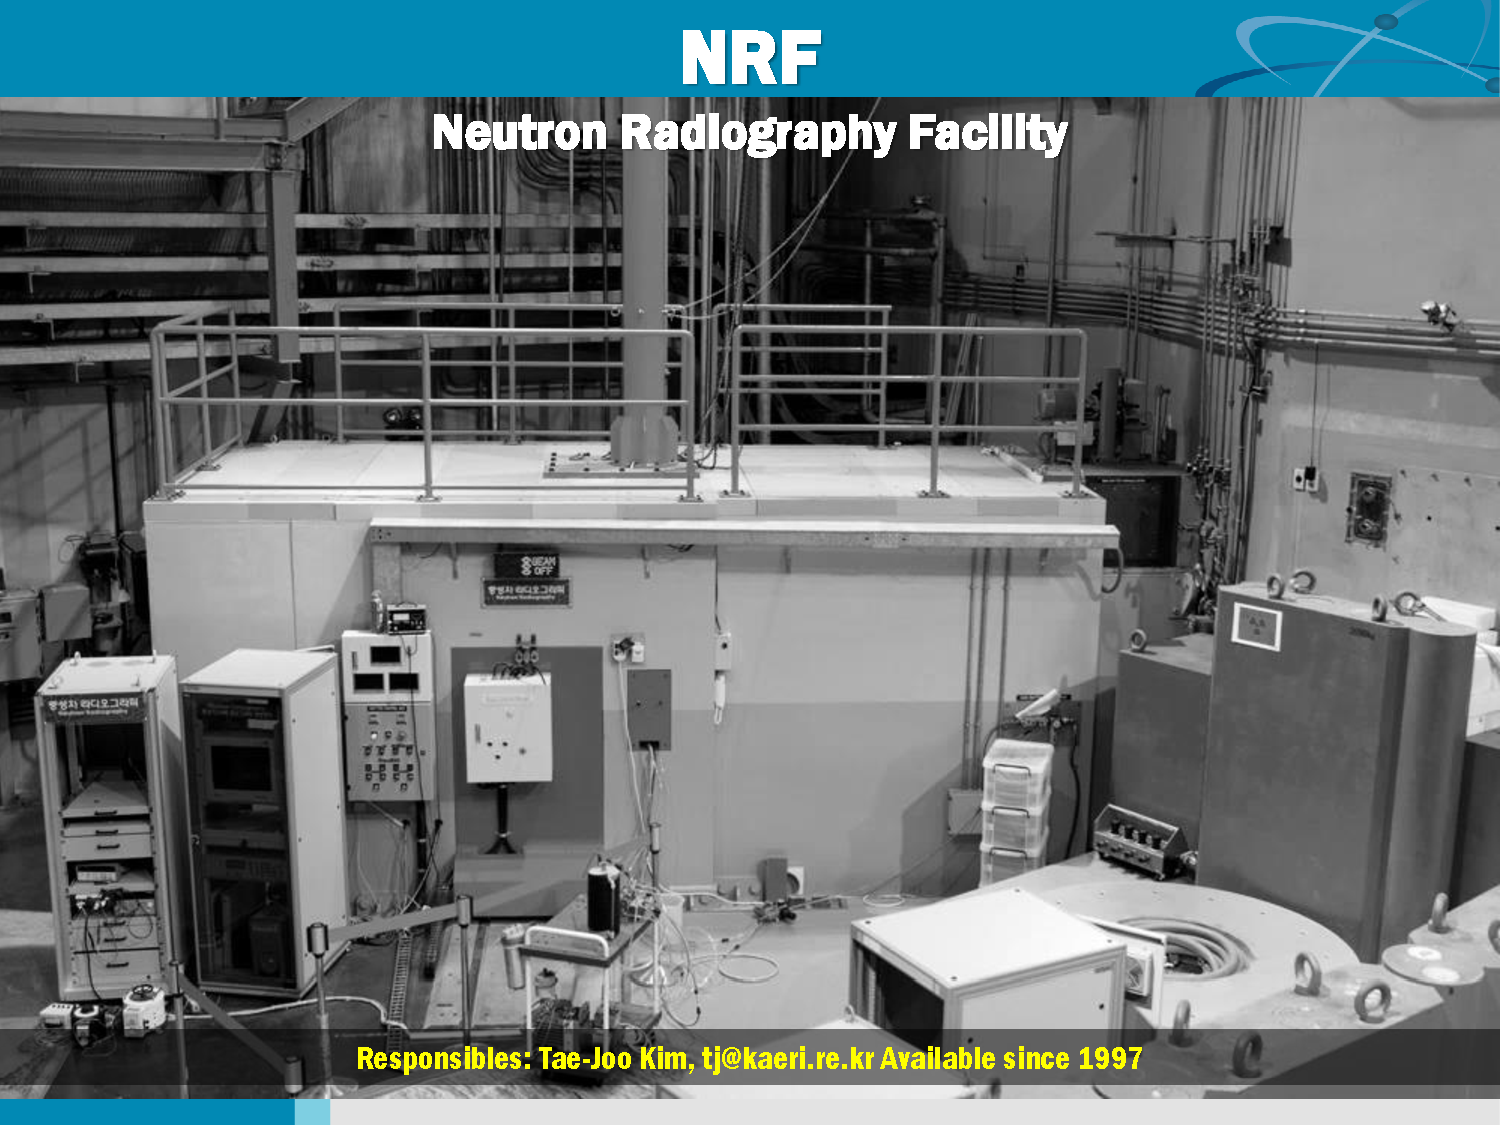
\includepdf{figures/pres2/sl-32.pdf}
\end{frame}

\begin{frame}
  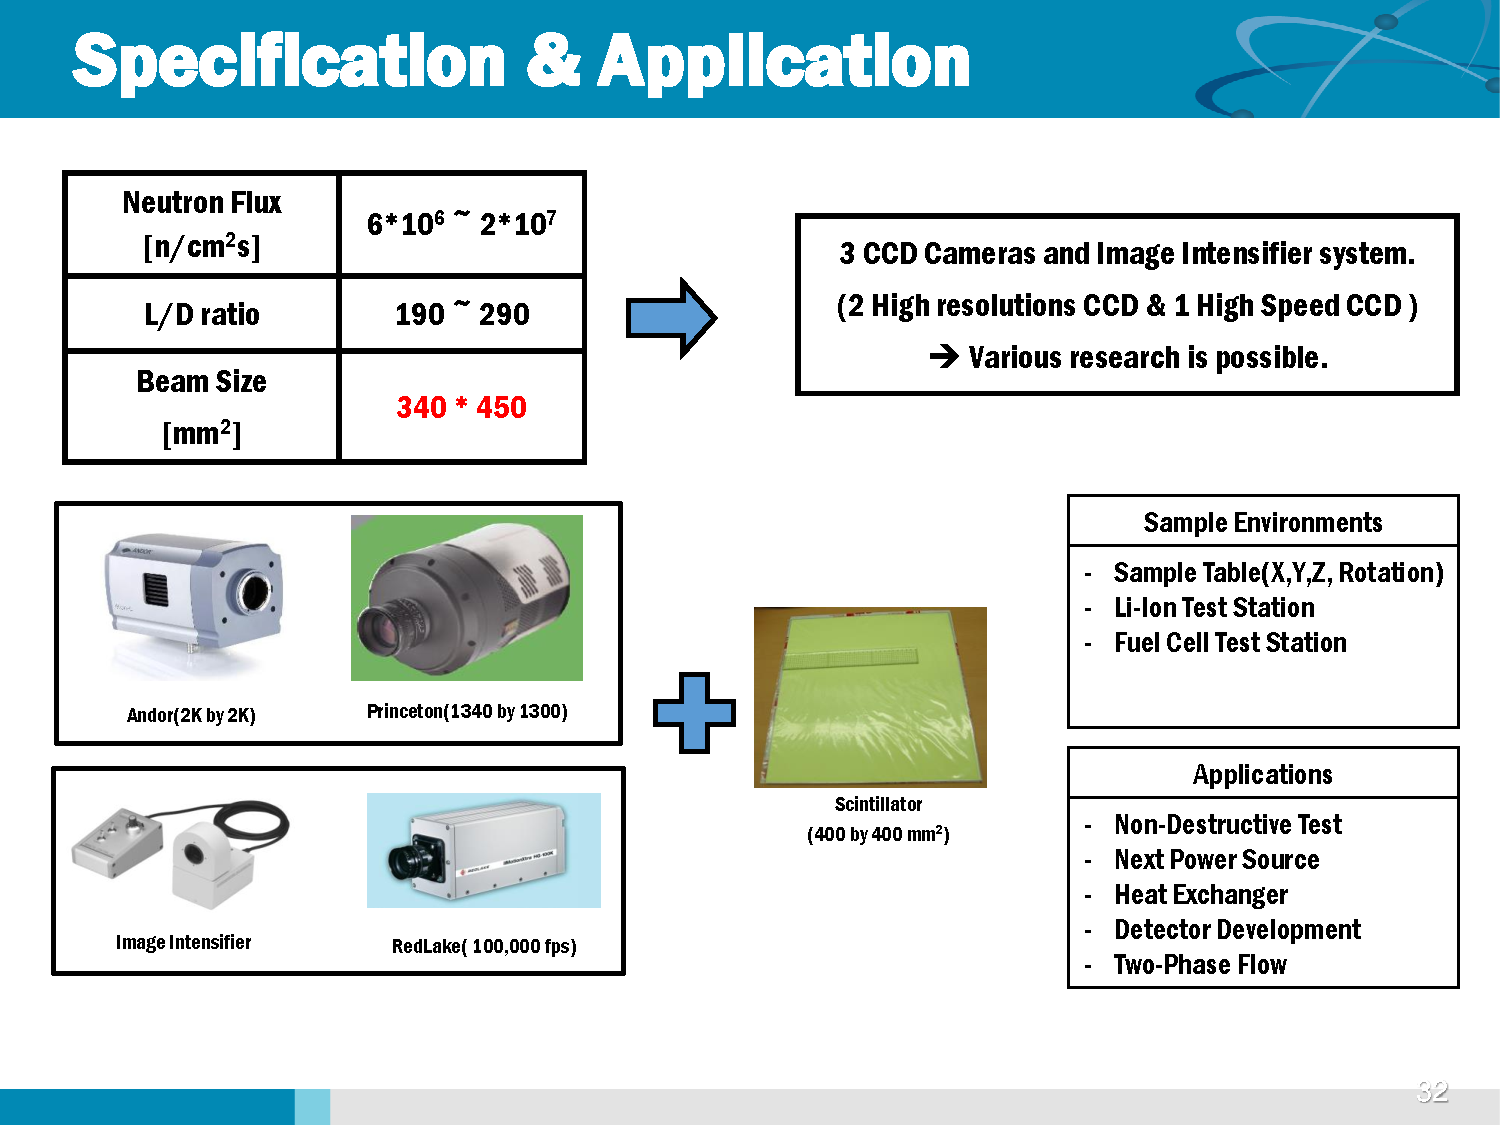
\includepdf{figures/pres2/sl-33.pdf}
\end{frame}

\begin{frame}
  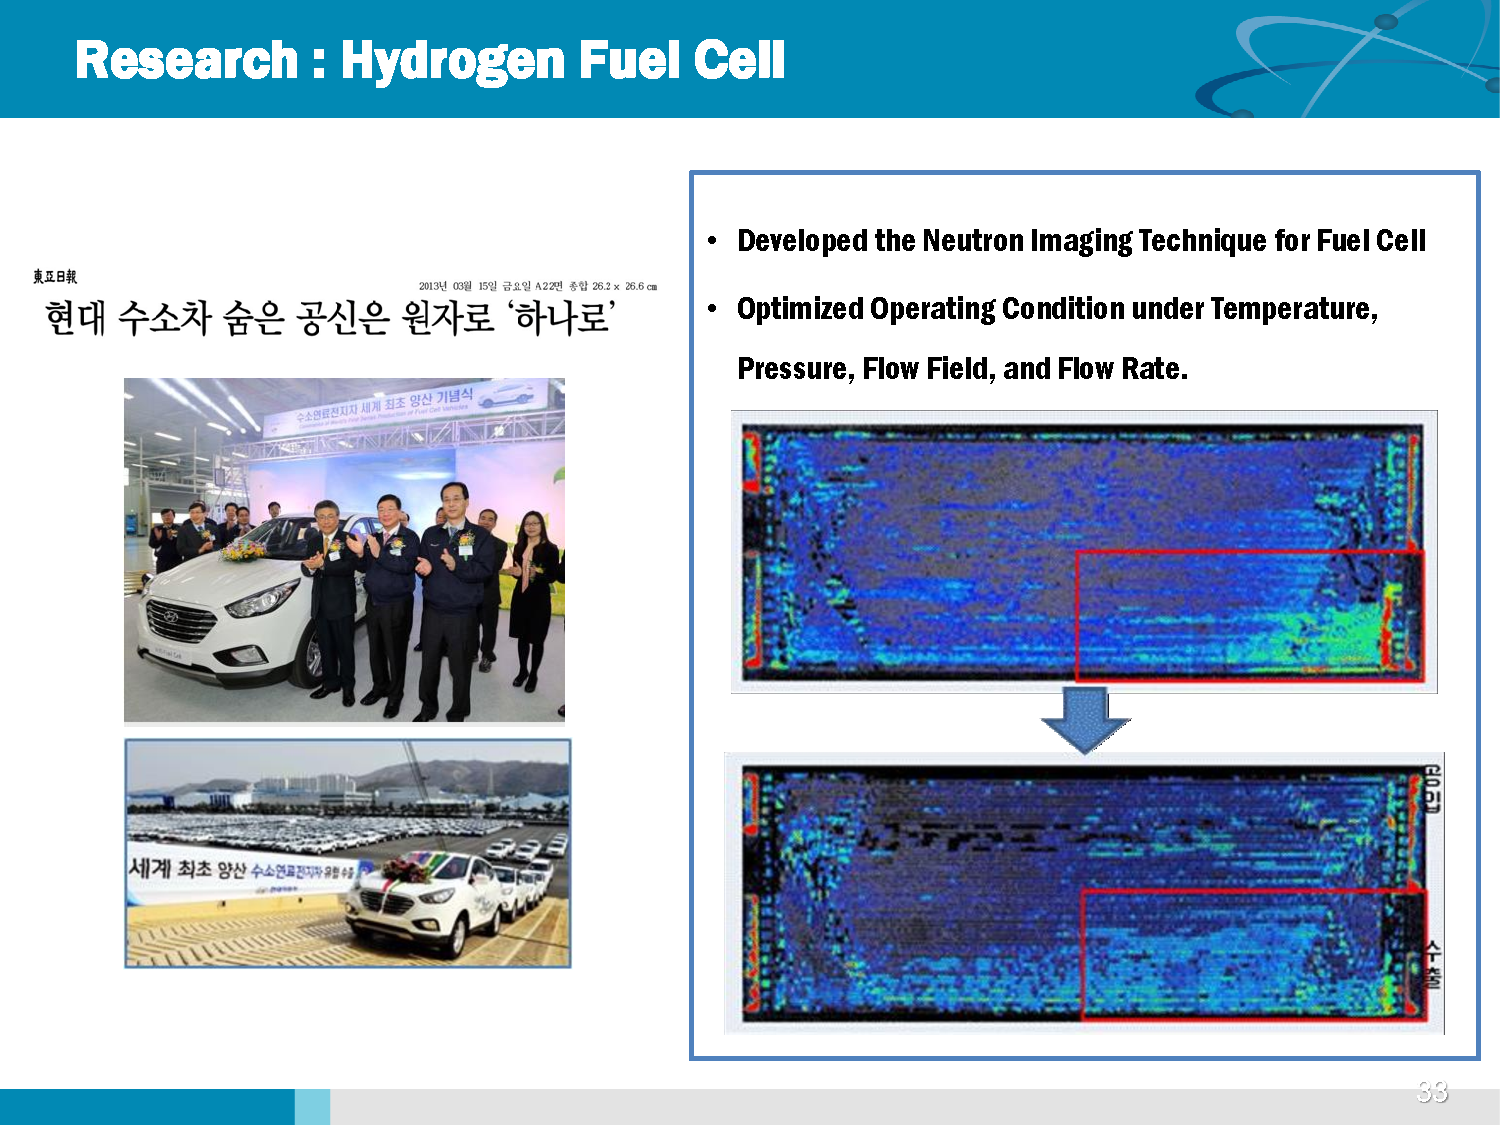
\includepdf{figures/pres2/sl-34.pdf}
\end{frame}

%-------------------------------------------------
\subsection{Instrumentation and Instrument Design for Neutron Imaging}
%-------------------------------------------------
\begin{frame}
  \frametitle{Apresentações escolhidas}
  \framesubtitle{(3)}
  \begin{center}
    Instrumentation and Instrument Design for Neutron Imaging\\
    \vspace{2.0cm}
    N. Kardjilov
  \end{center}
\end{frame}

\begin{frame}
  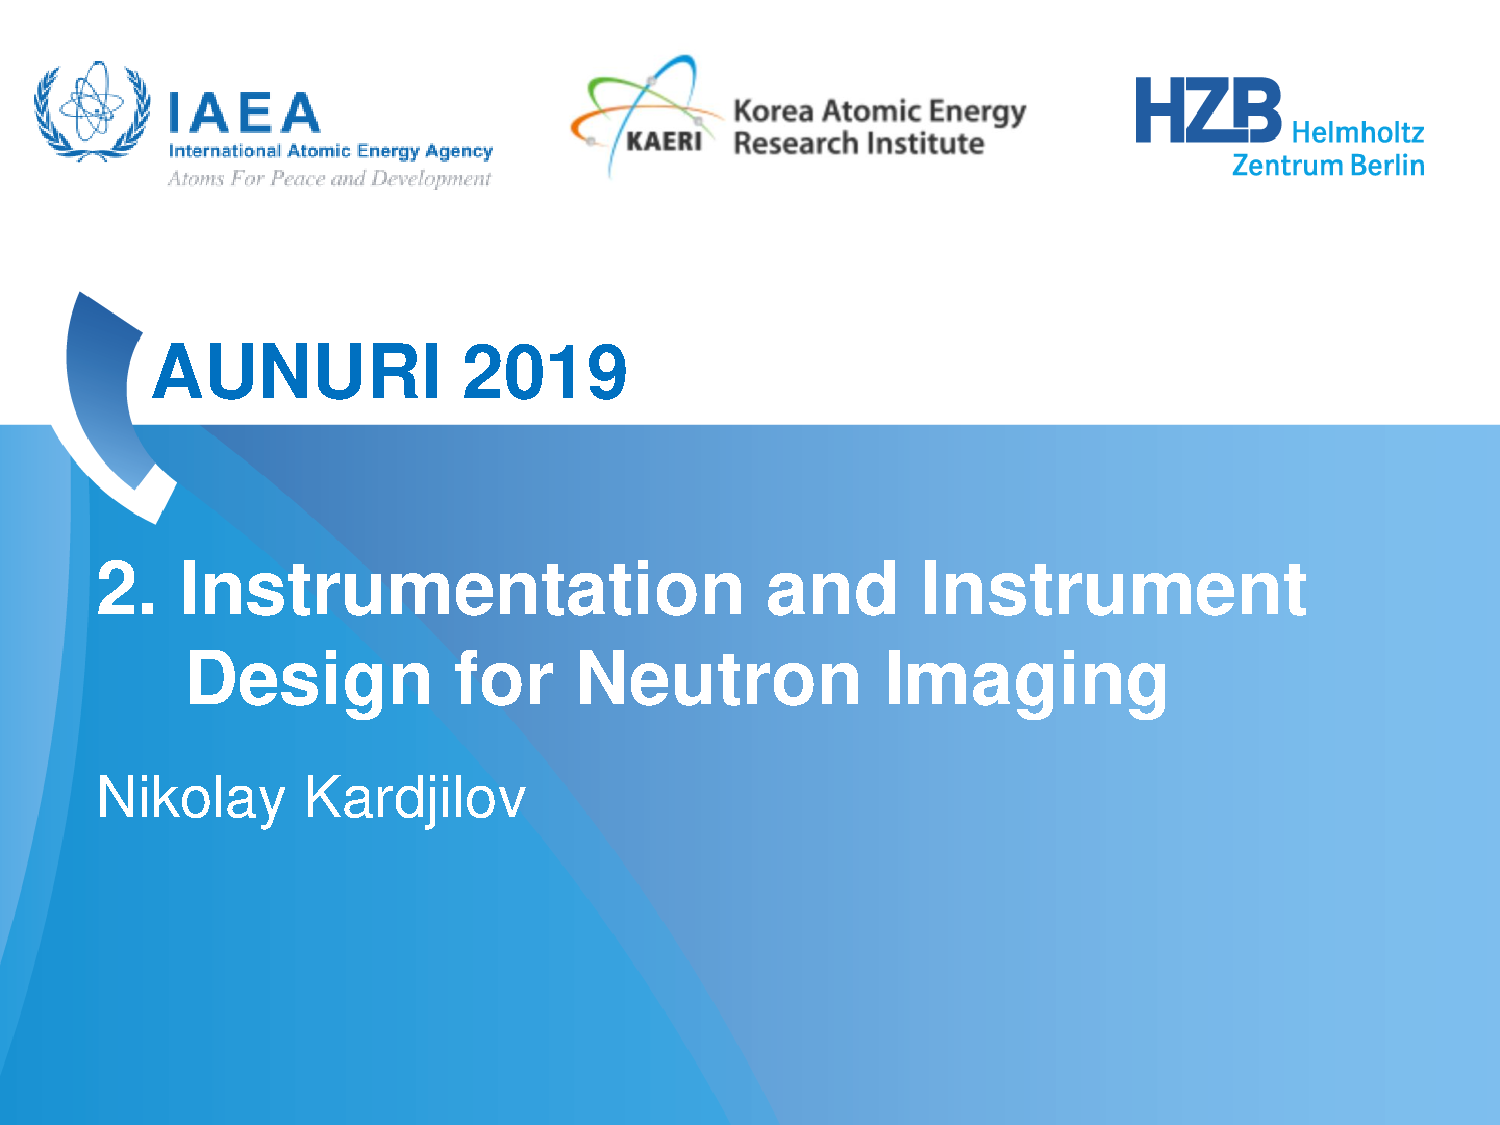
\includepdf{figures/pres3/sl-1.pdf}
\end{frame}
\begin{frame}
  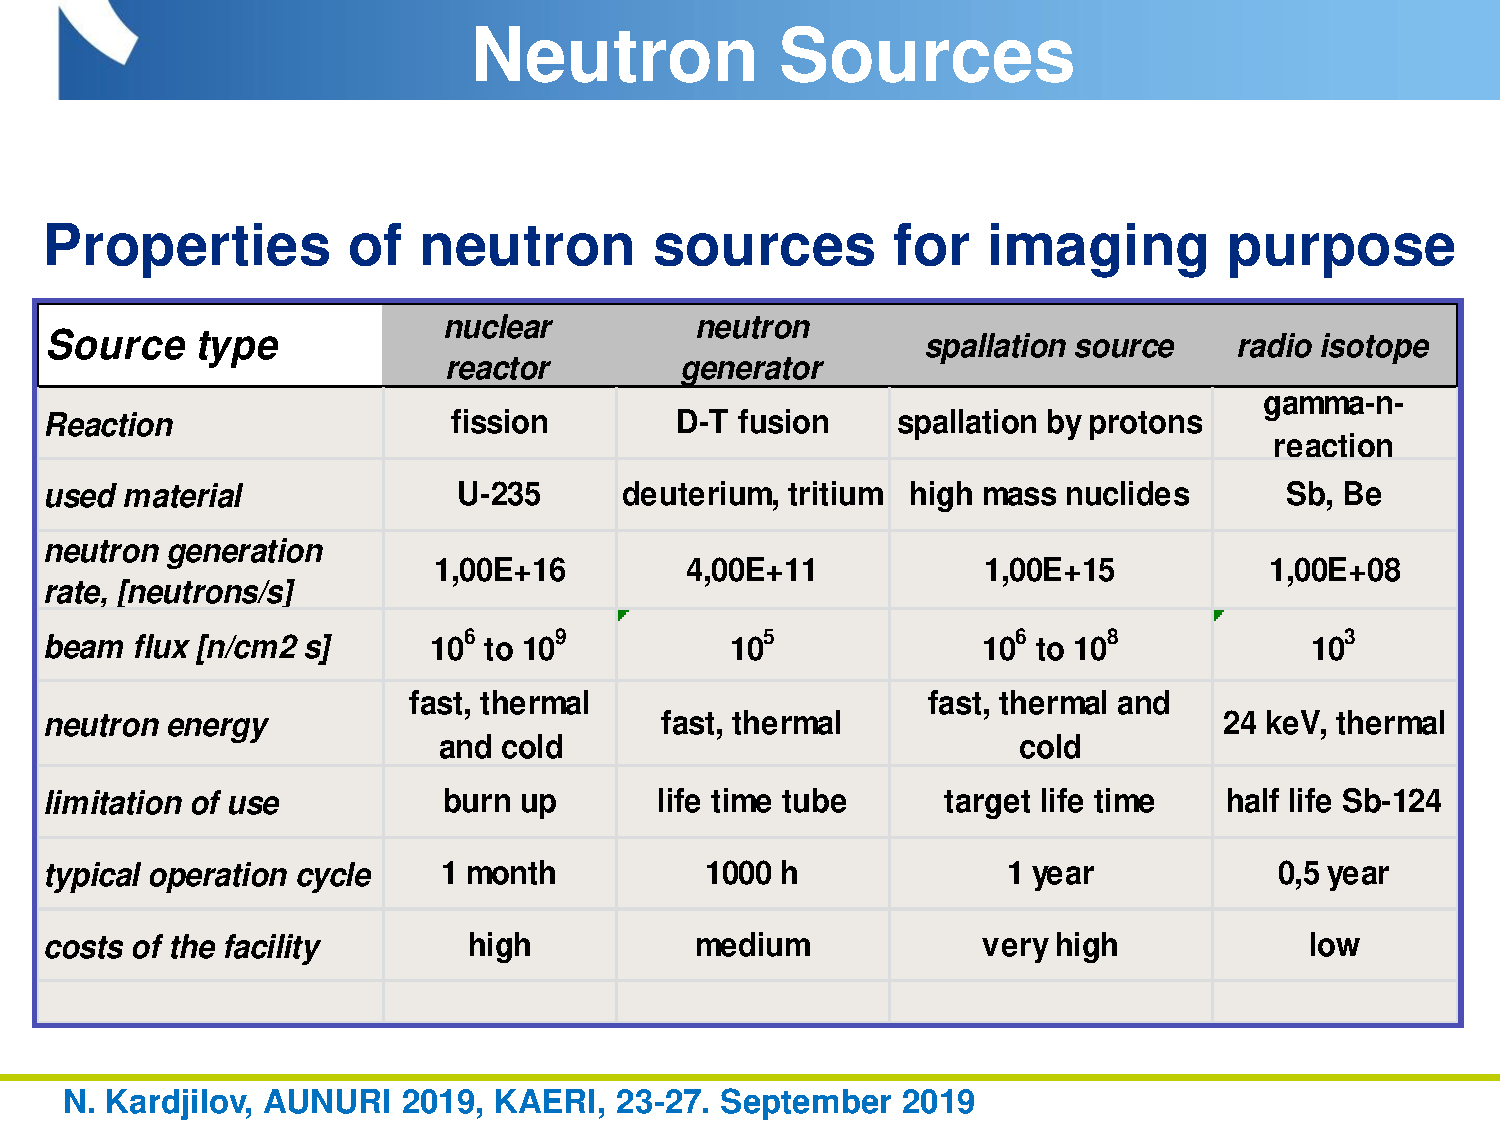
\includepdf{figures/pres3/sl-4.pdf}
\end{frame}
\begin{frame}
  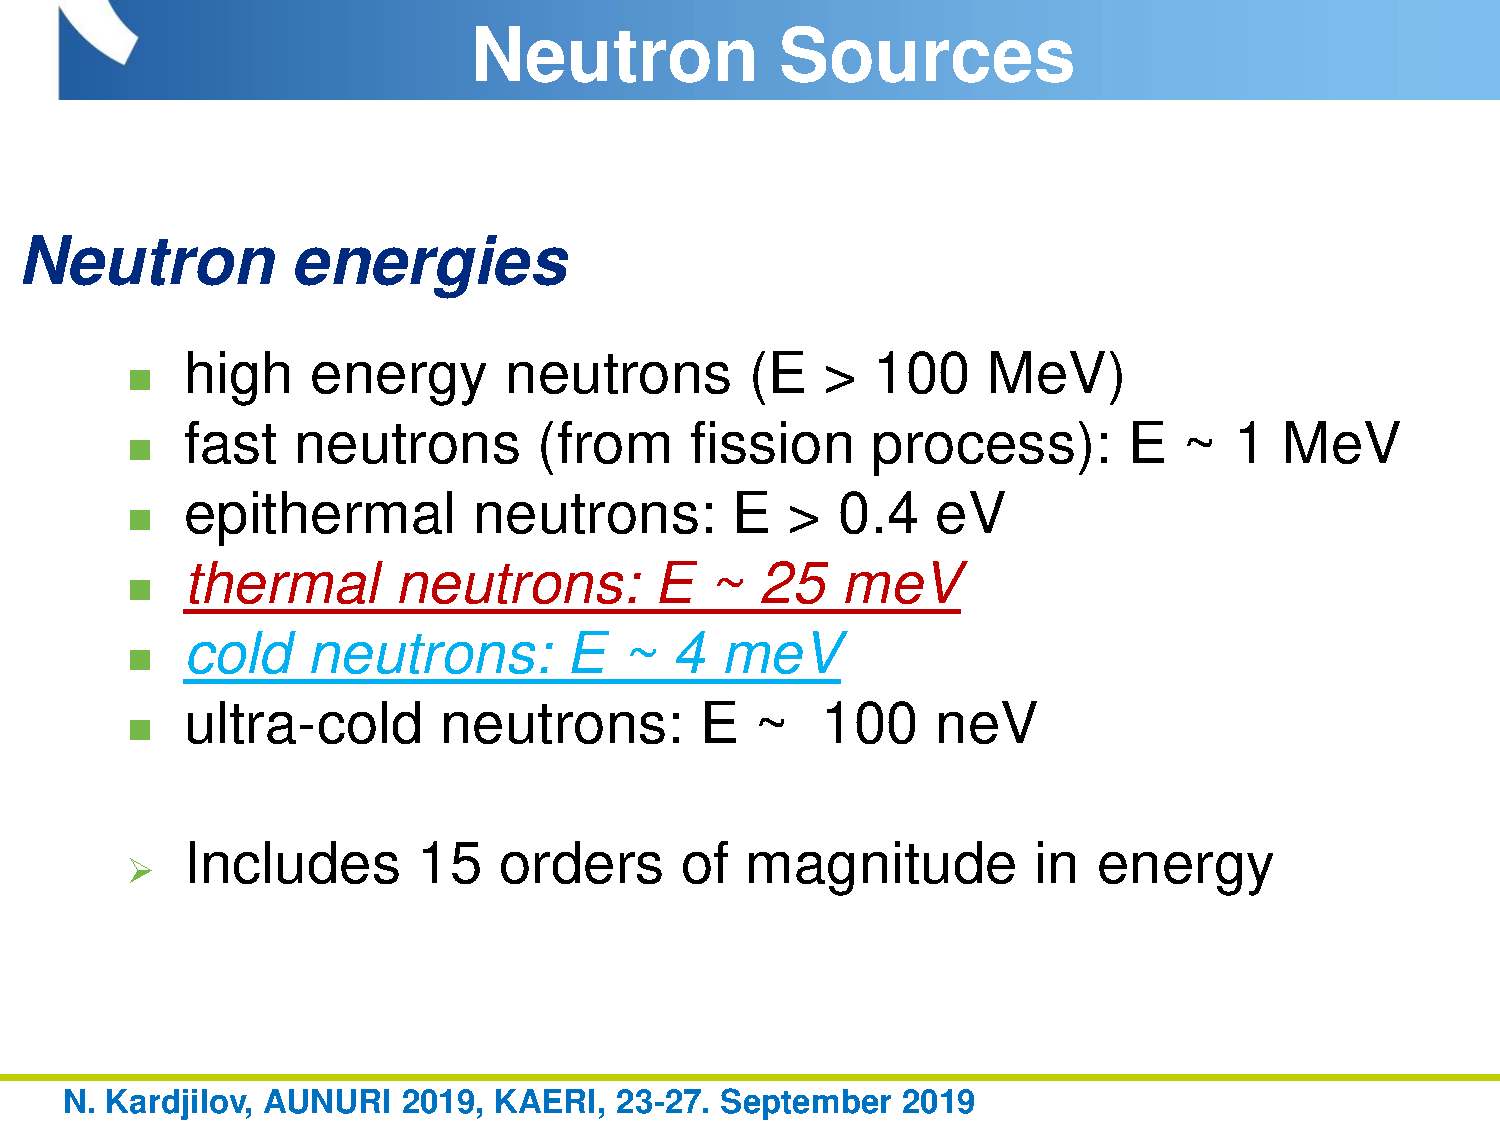
\includepdf{figures/pres3/sl-5.pdf}
\end{frame}
\begin{frame}
  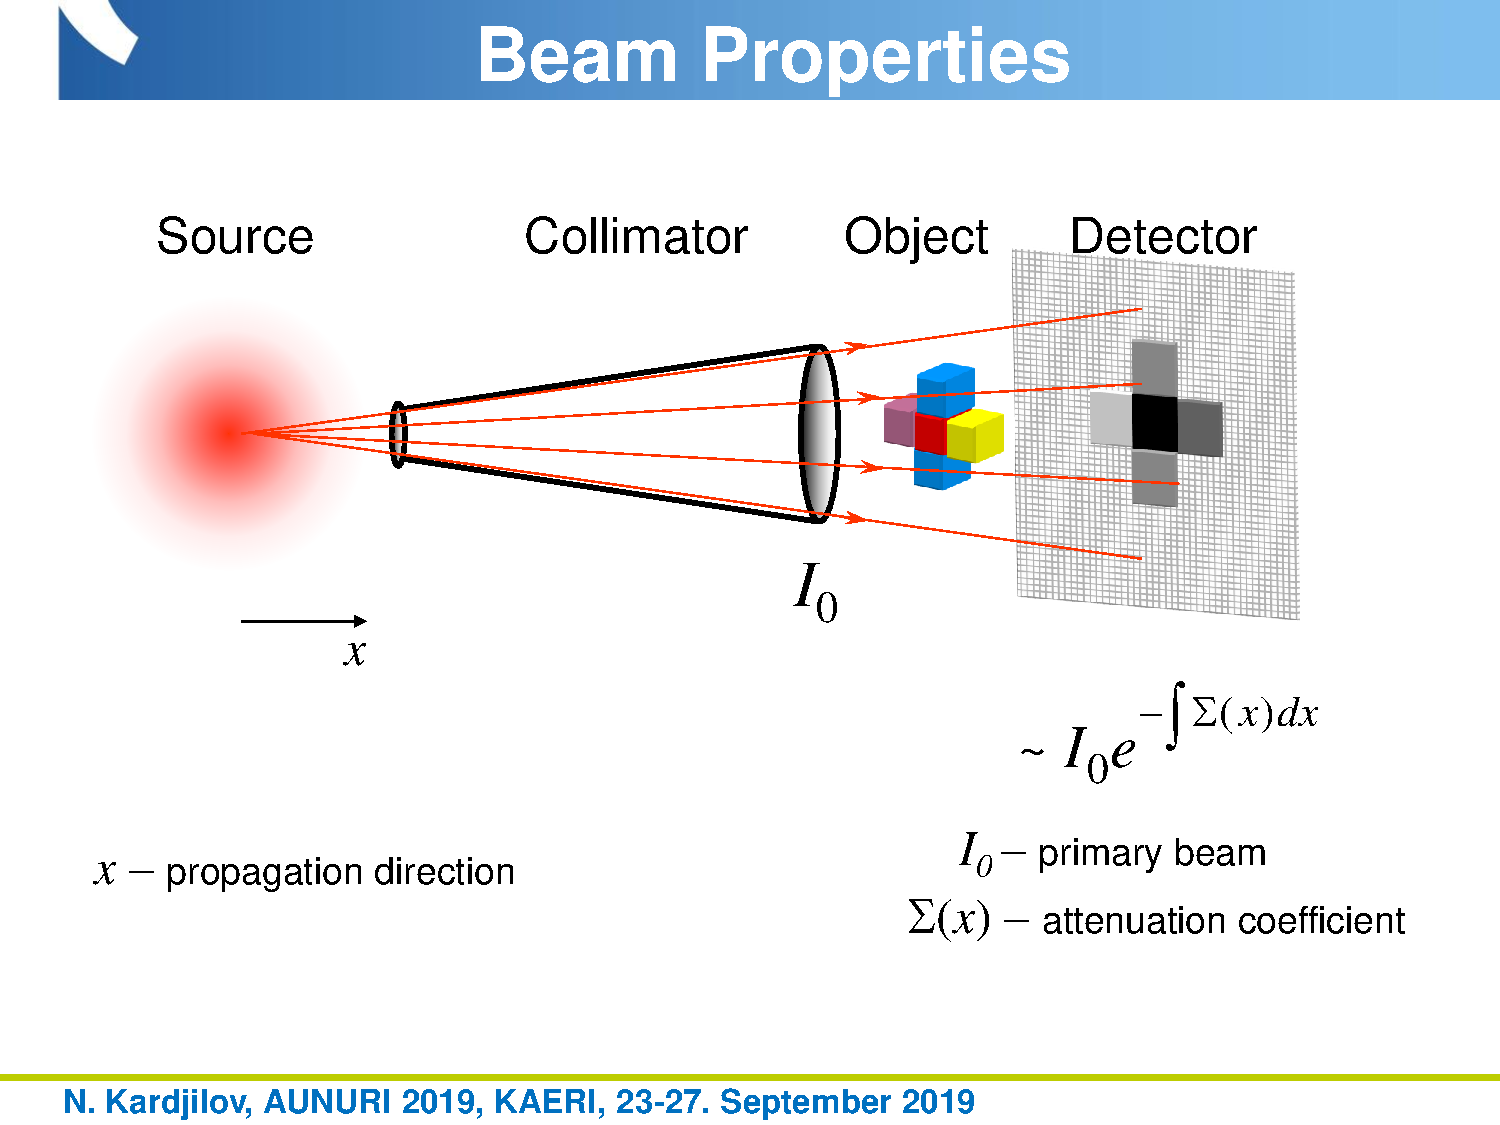
\includepdf{figures/pres3/sl-14.pdf}
\end{frame}
\begin{frame}
  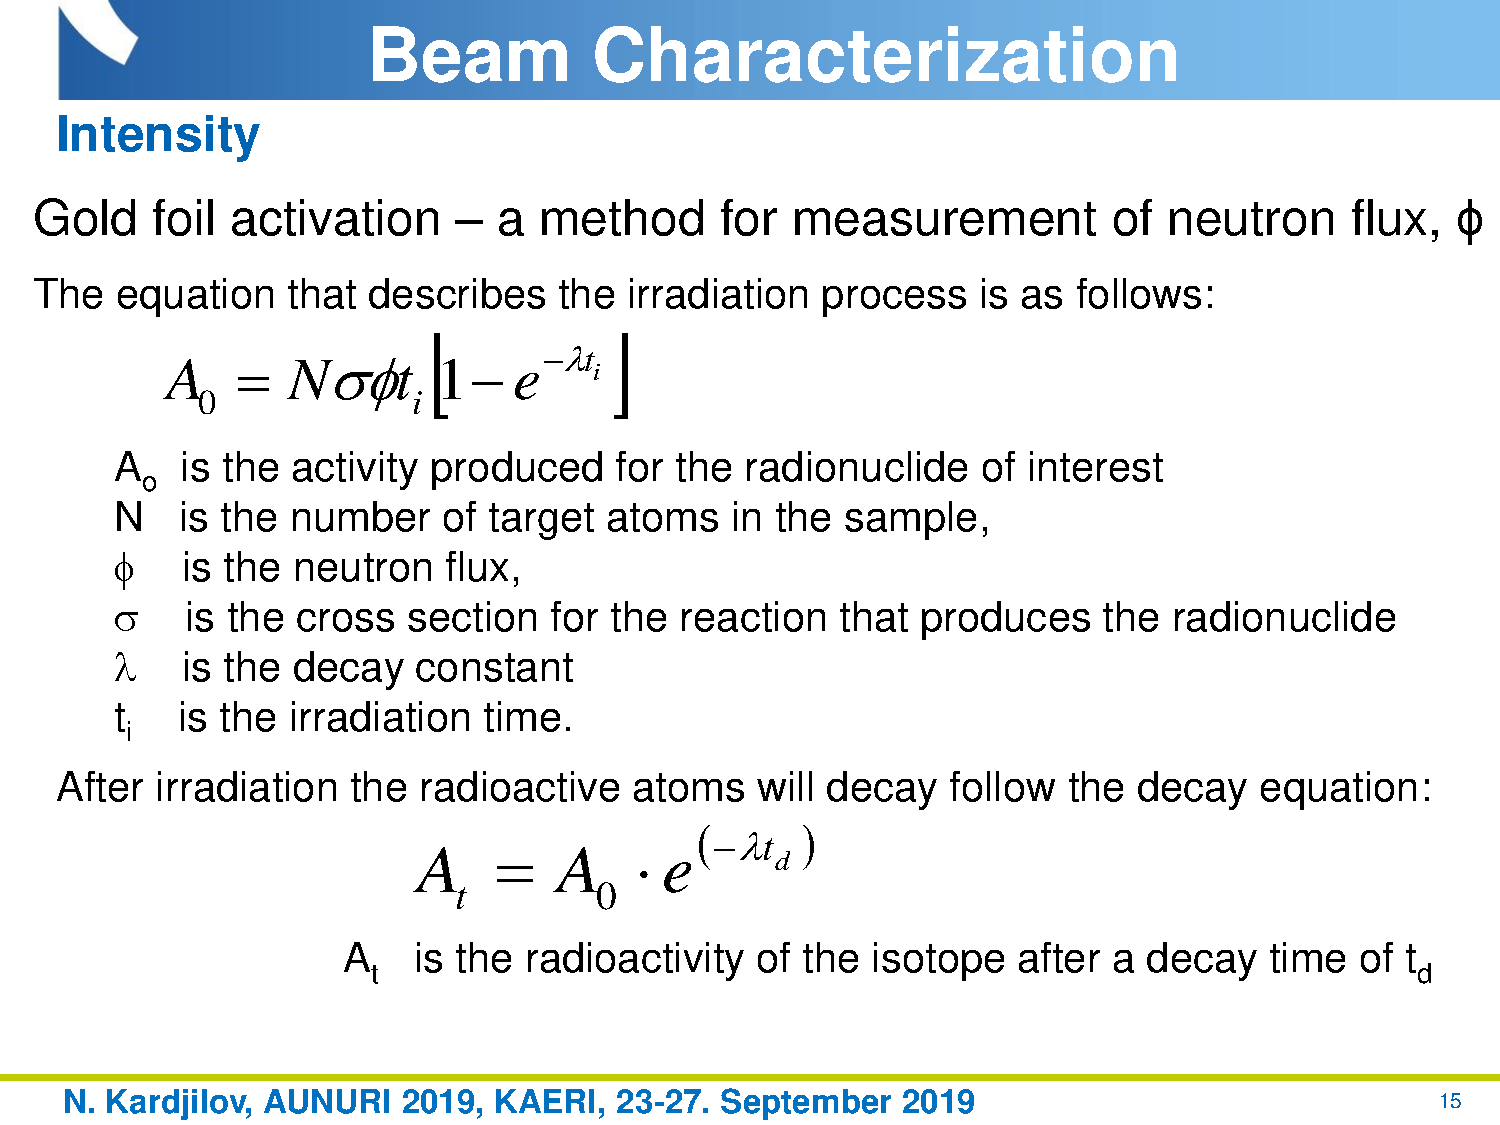
\includepdf{figures/pres3/sl-15.pdf}
\end{frame}
\begin{frame}
  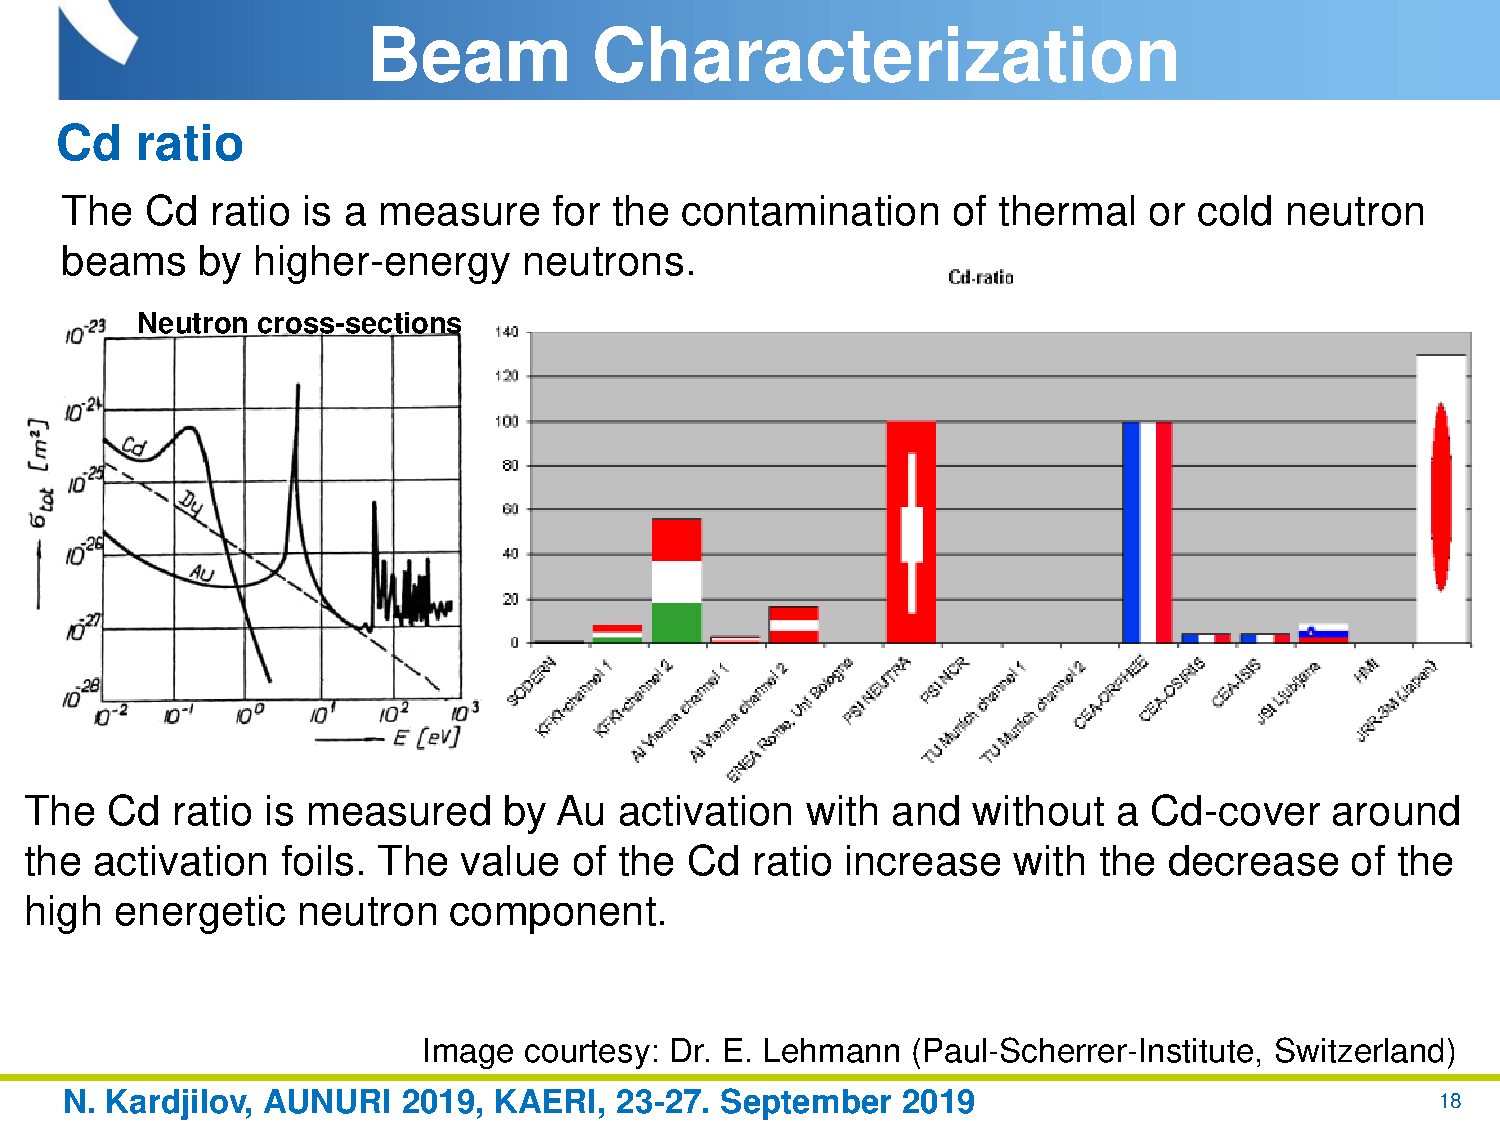
\includepdf{figures/pres3/sl-18.pdf}
\end{frame}
\begin{frame}
  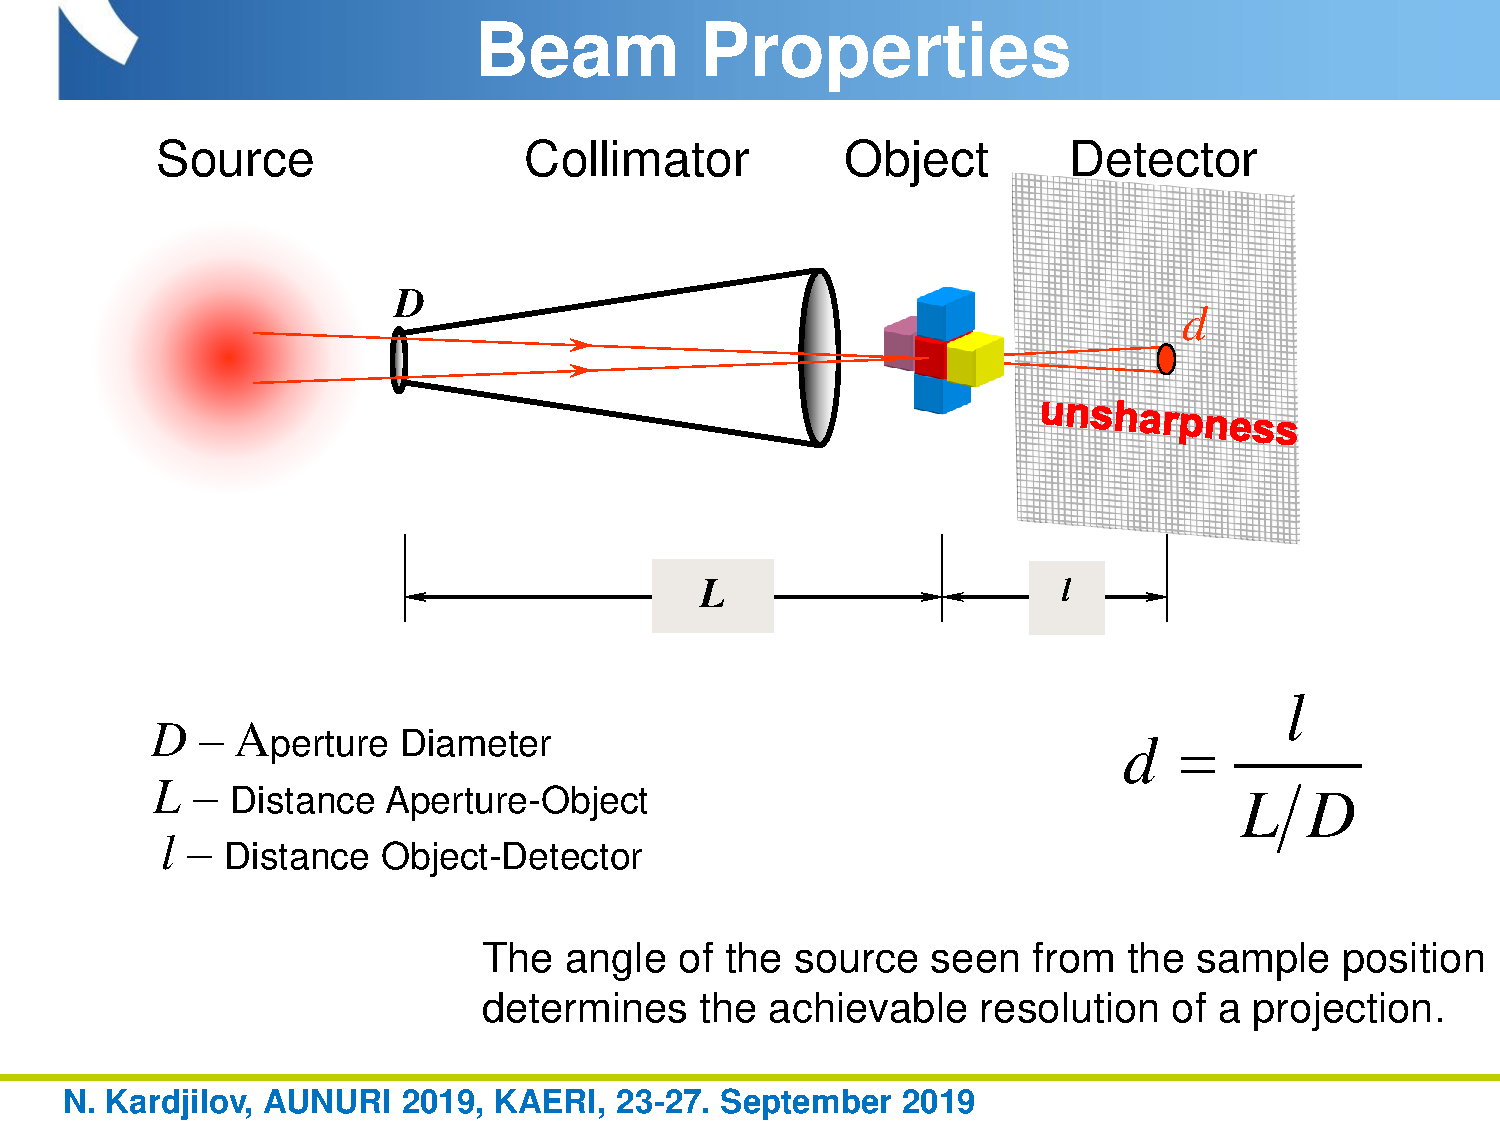
\includepdf{figures/pres3/sl-19.pdf}
\end{frame}
\begin{frame}
  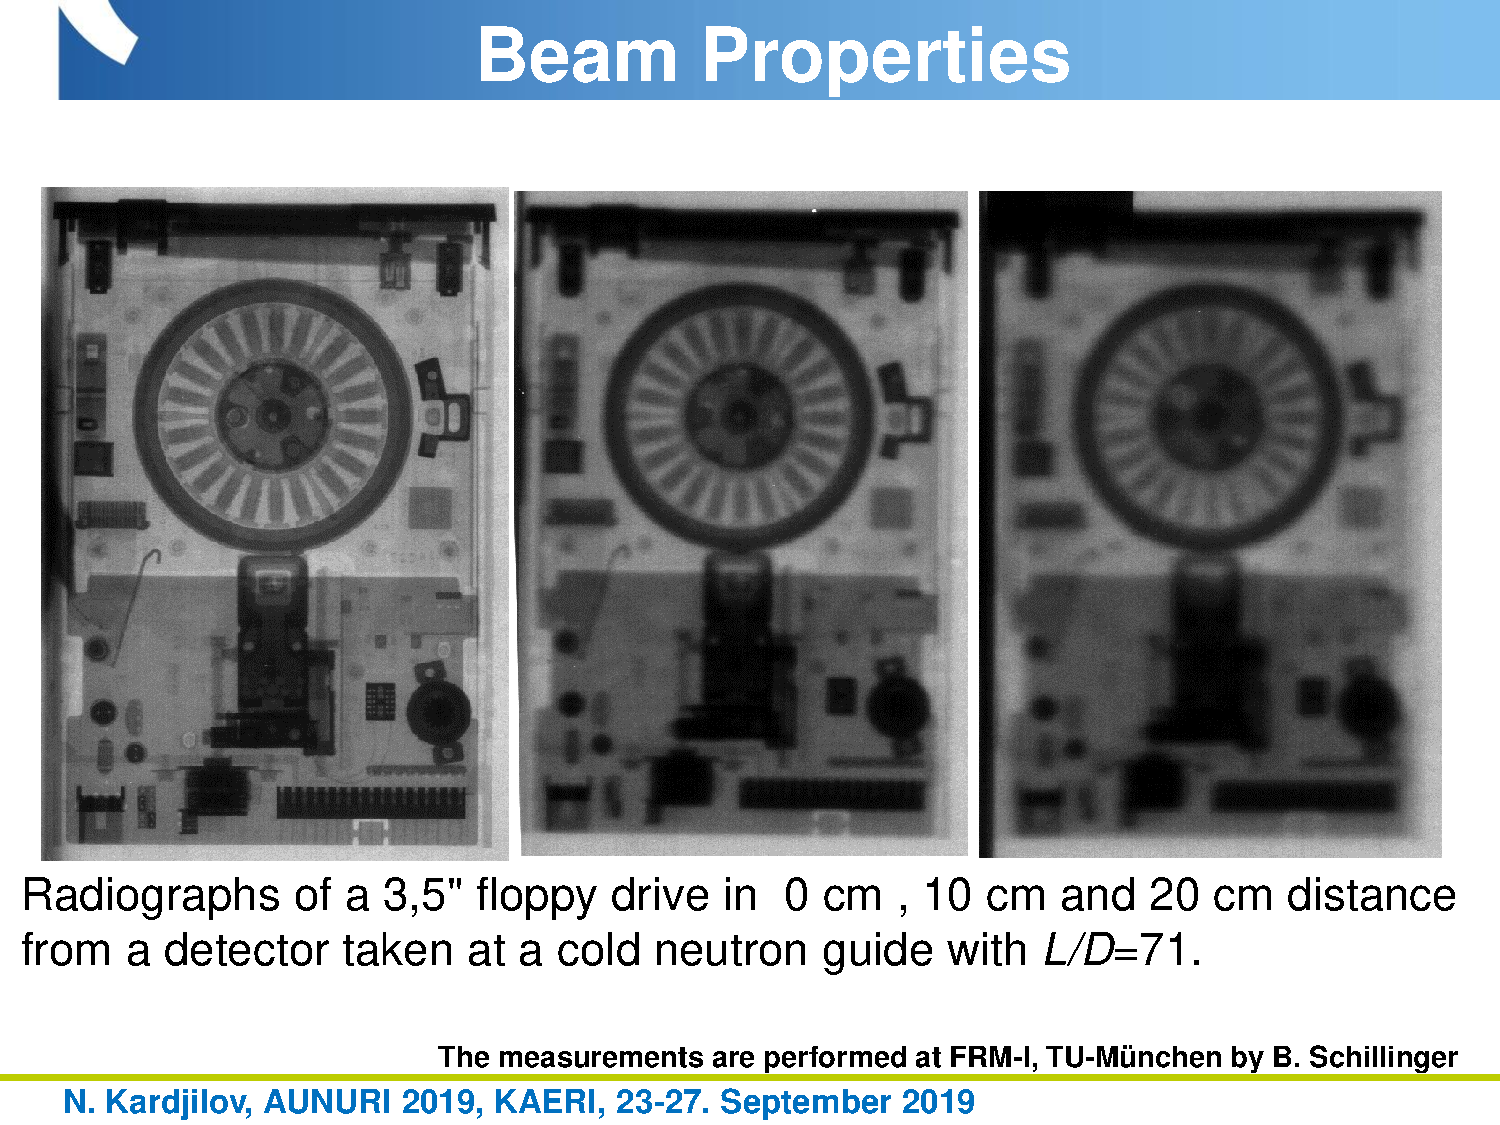
\includepdf{figures/pres3/sl-20.pdf}
\end{frame}
\begin{frame}
  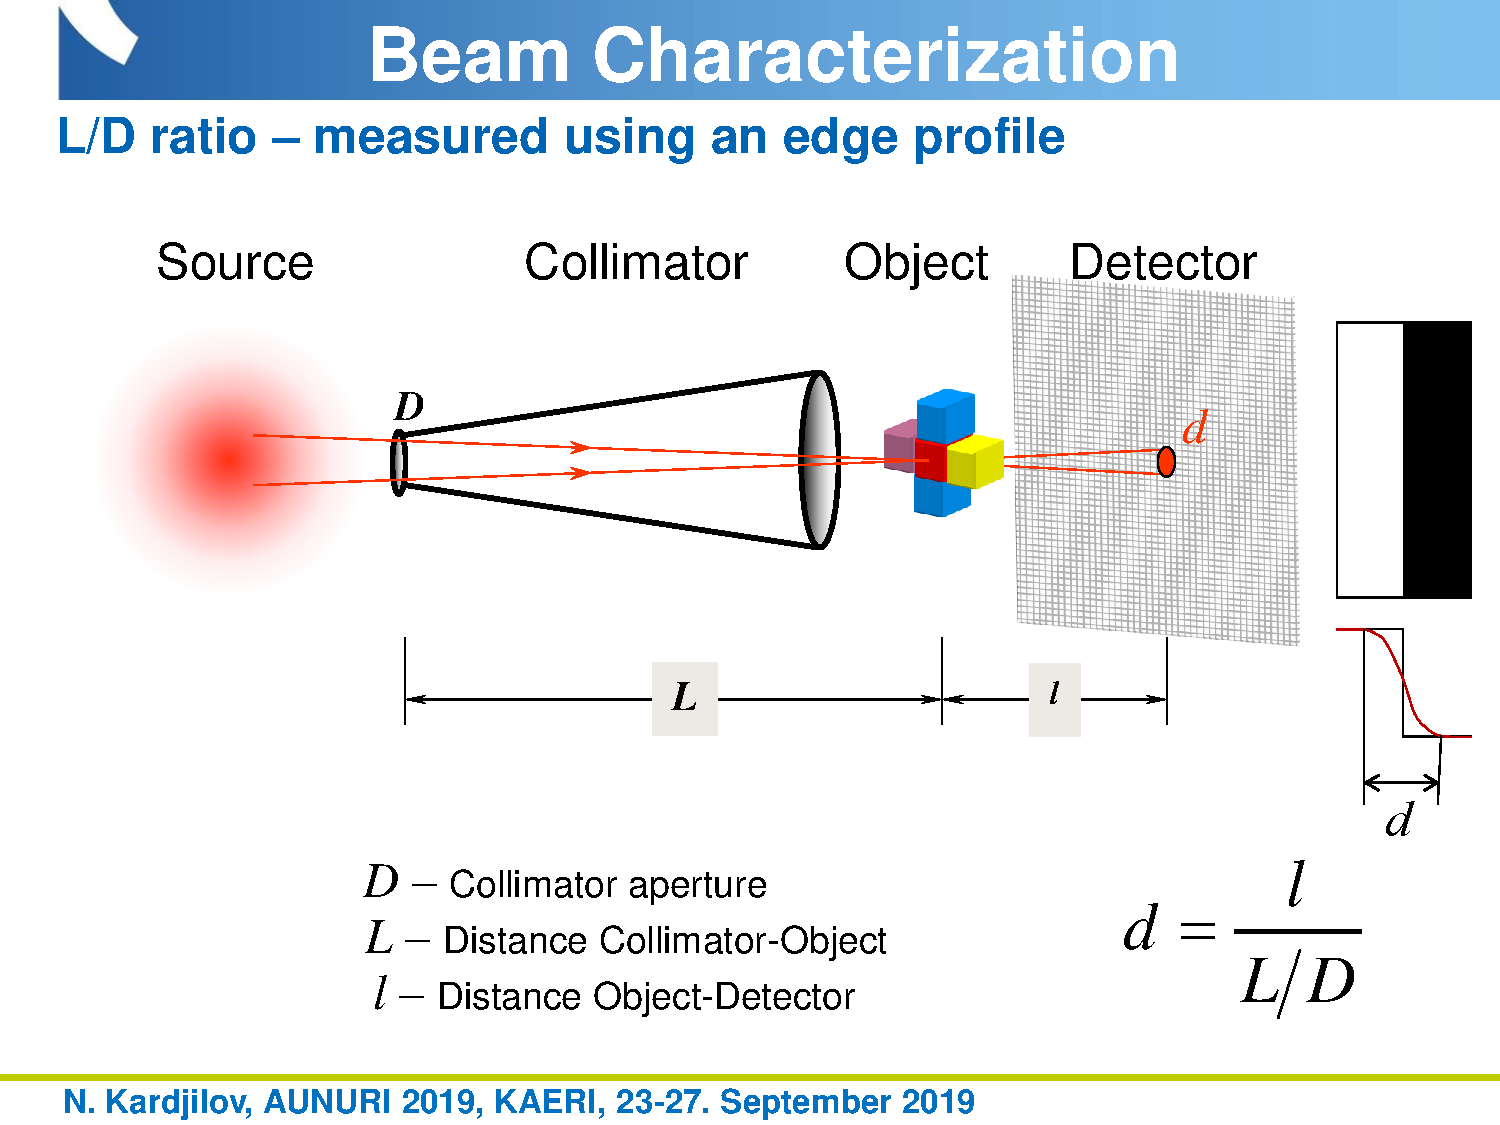
\includepdf{figures/pres3/sl-22.pdf}
\end{frame}
\begin{frame}
  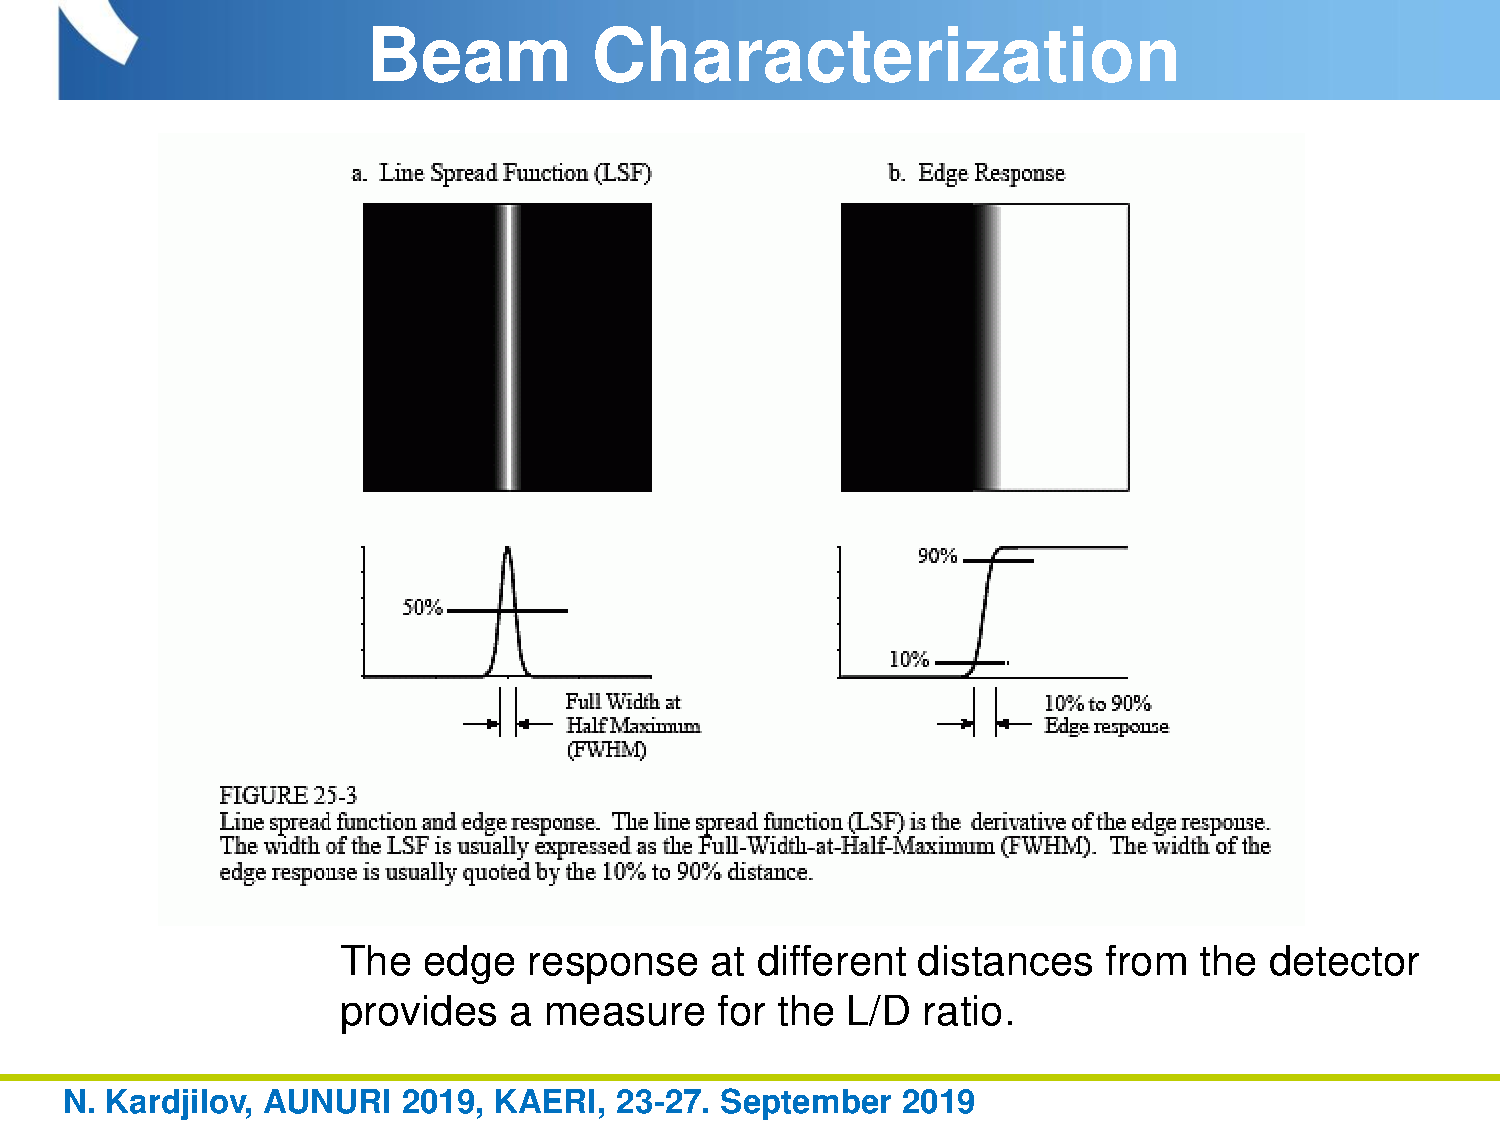
\includepdf{figures/pres3/sl-23.pdf}
\end{frame}
\begin{frame}
  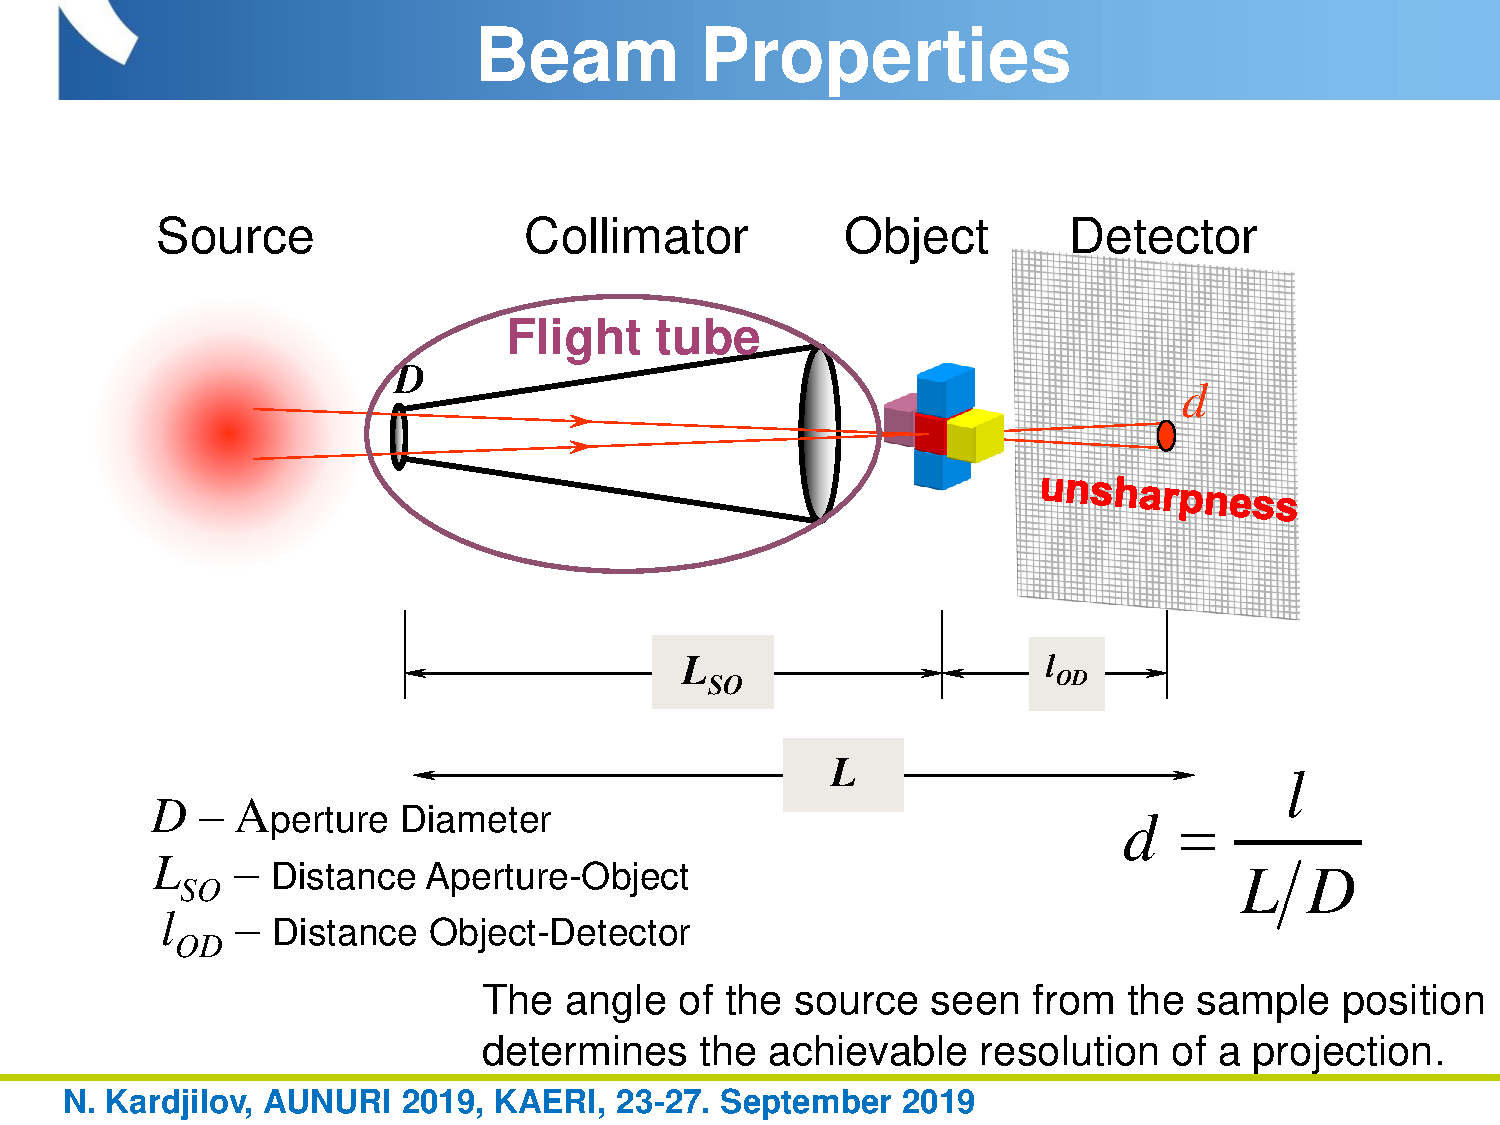
\includepdf{figures/pres3/sl-25.pdf}
\end{frame}
\begin{frame}
  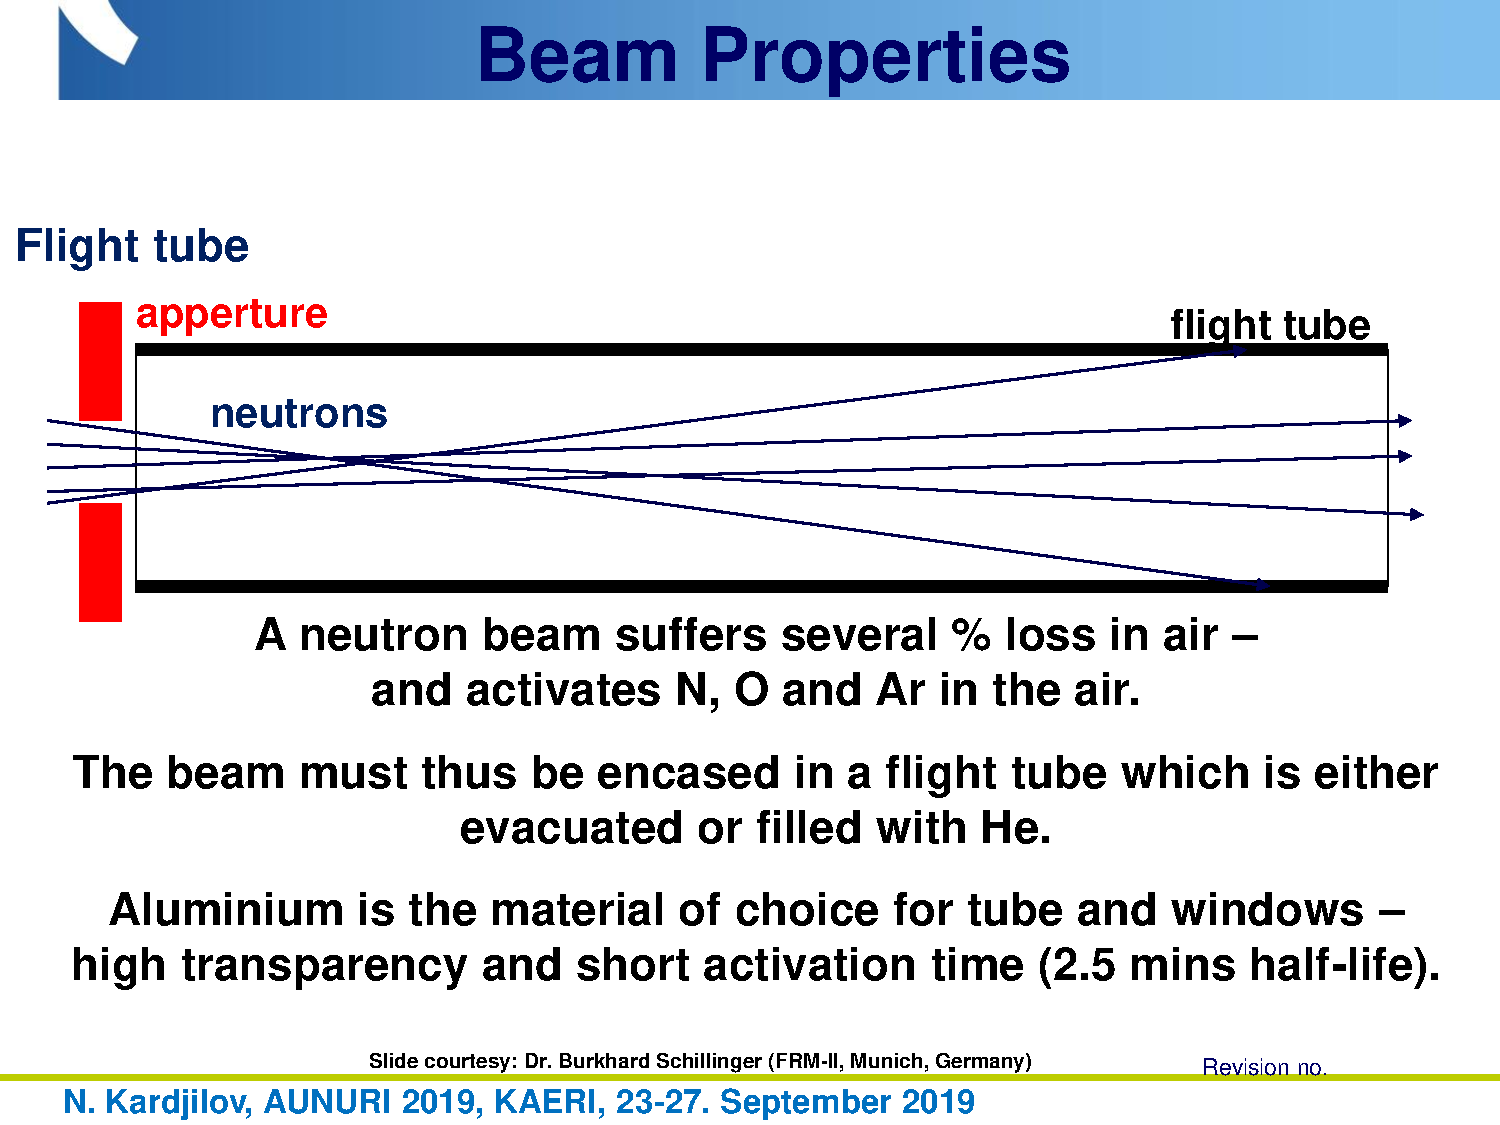
\includepdf{figures/pres3/sl-26.pdf}
\end{frame}
\begin{frame}
  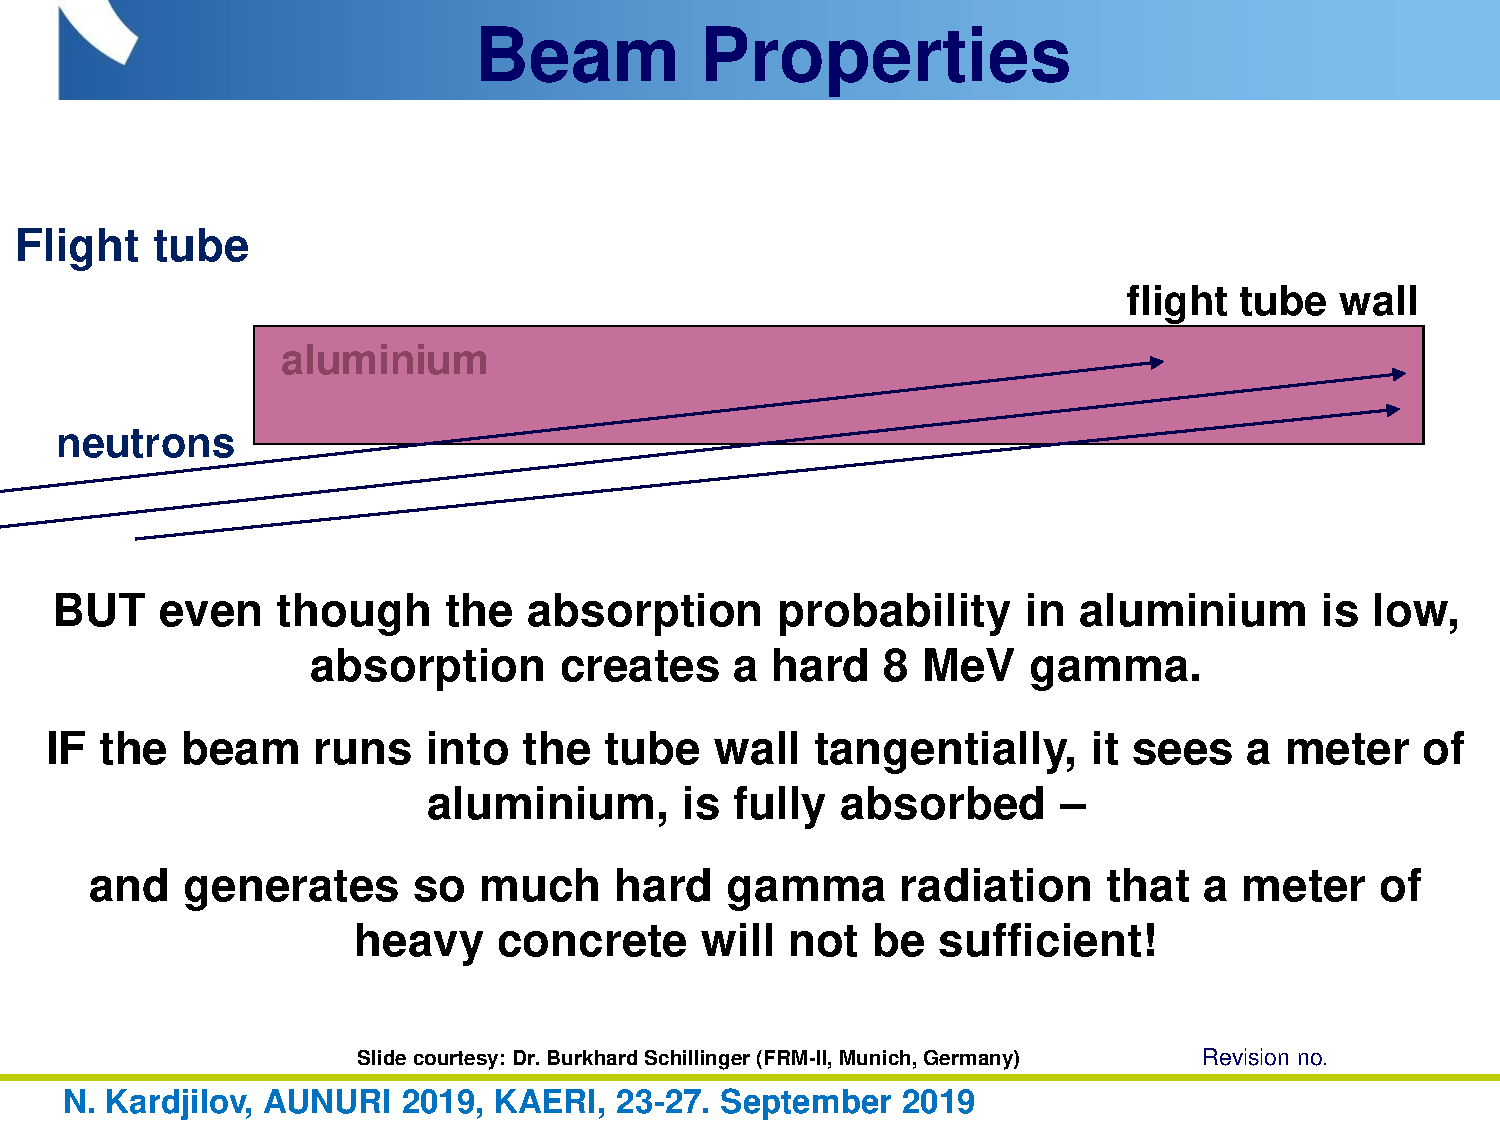
\includepdf{figures/pres3/sl-27.pdf}
\end{frame}
\begin{frame}
  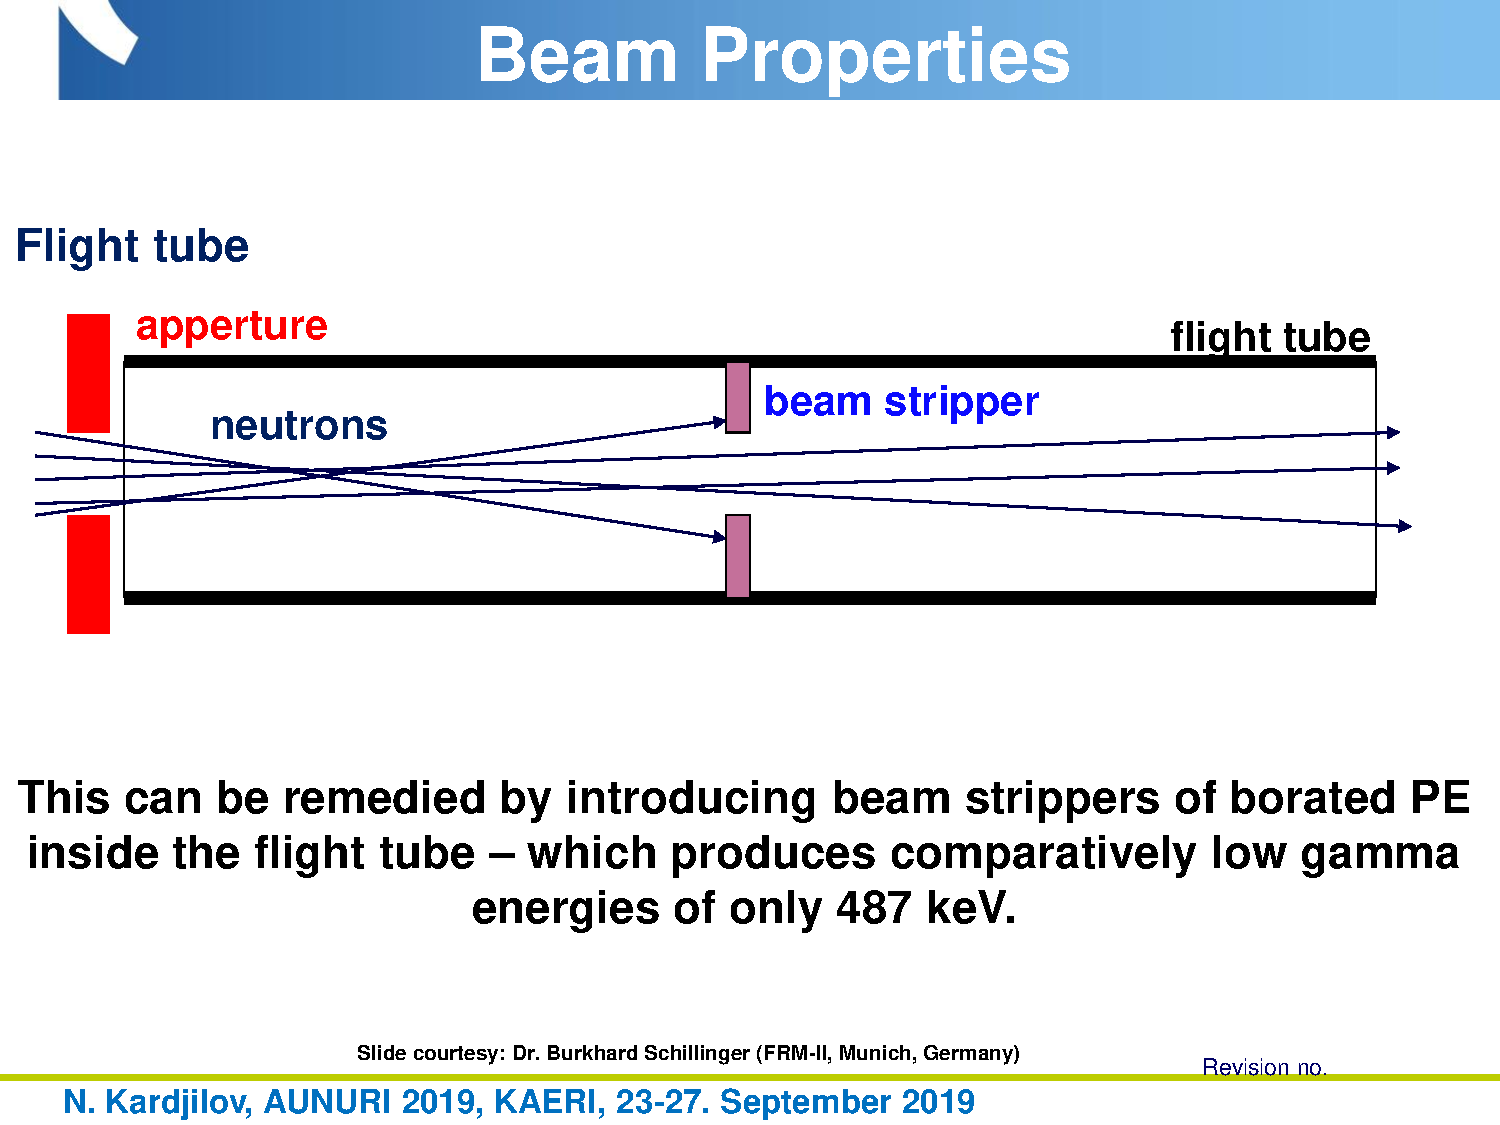
\includepdf{figures/pres3/sl-28.pdf}
\end{frame}

%-------------------------------------------------
\subsection{Detectors for Neutron Imaging}
%-------------------------------------------------
\begin{frame}
  \frametitle{Apresentações escolhidas}
  \framesubtitle{(4)}
  \begin{center}
    Detectors for Neutron Imaging\\
    \vspace{2.0cm}
    N. Kardjilov
  \end{center}
\end{frame}

\begin{frame}
  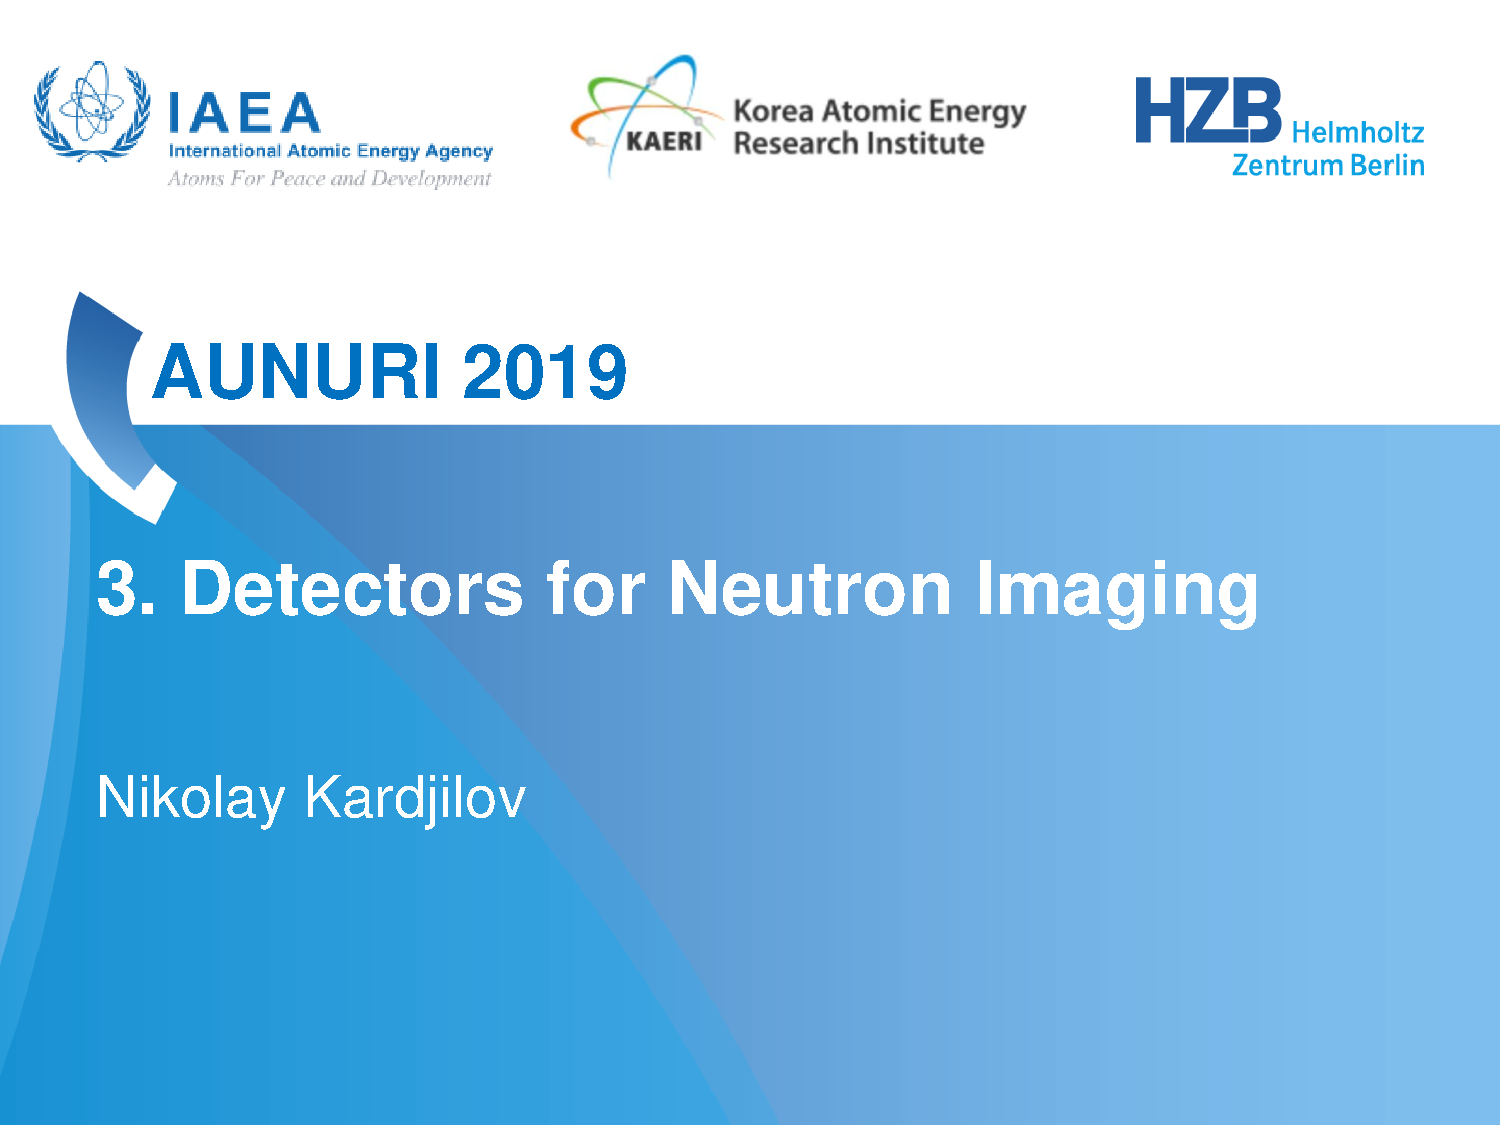
\includepdf{figures/pres4/sl-1.pdf}
\end{frame}
\begin{frame}
  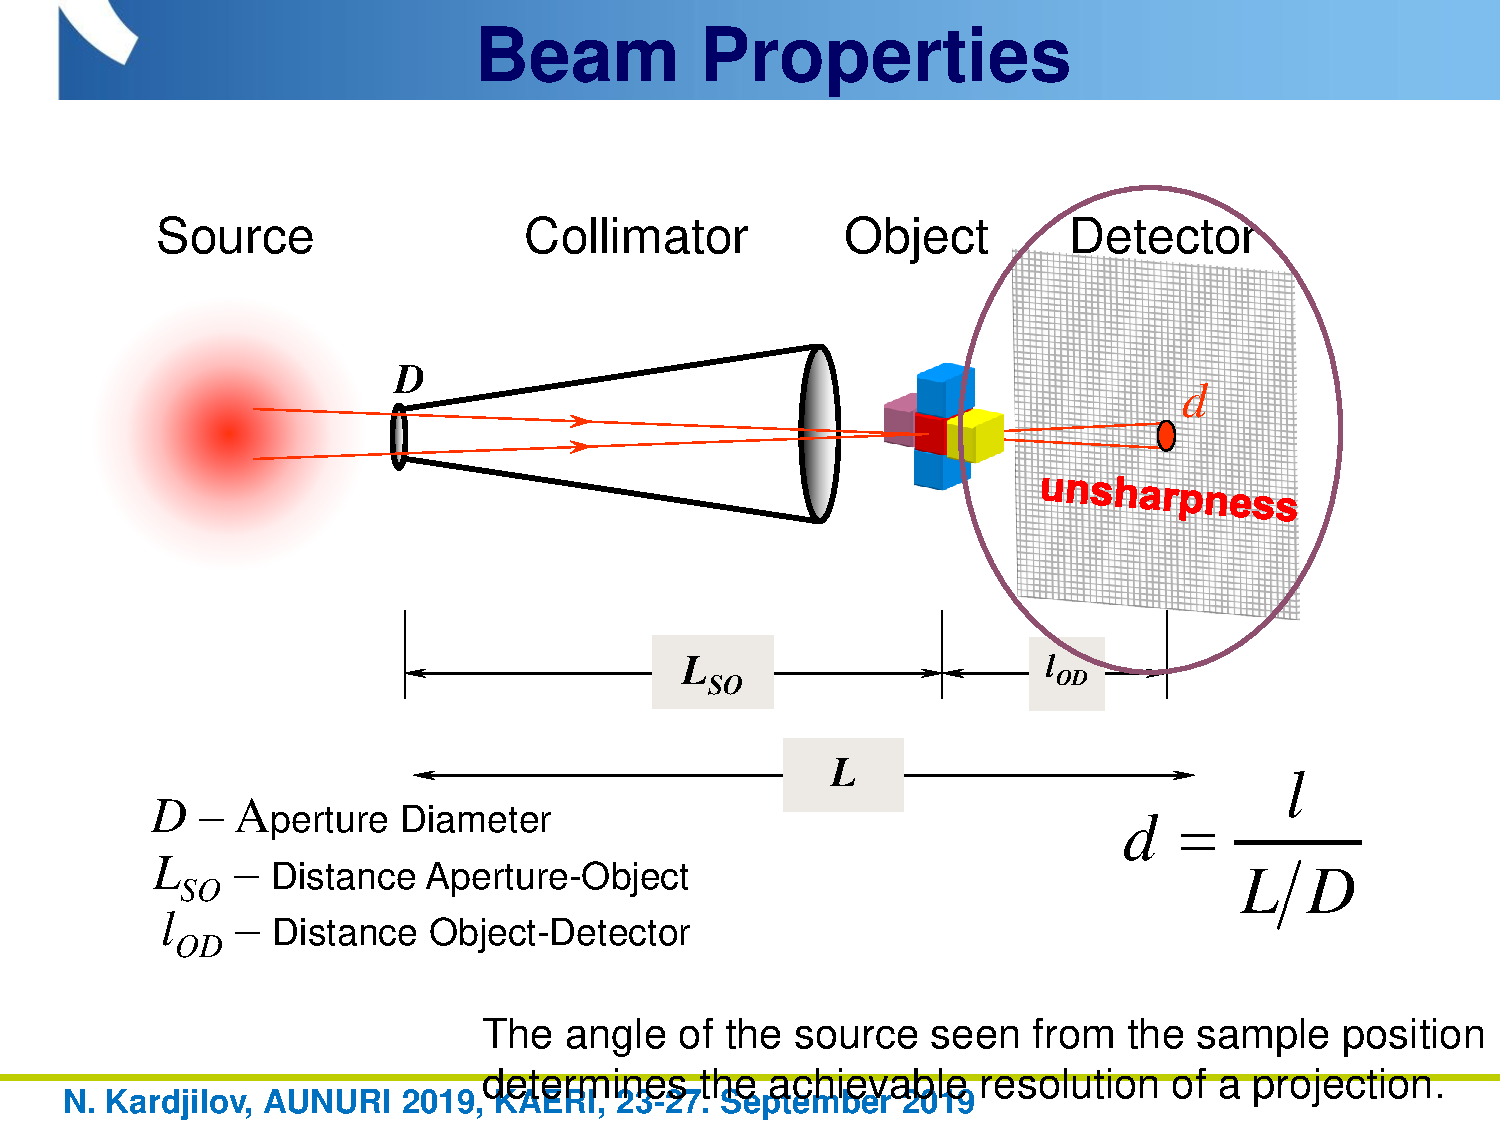
\includepdf{figures/pres4/sl-3.pdf}
\end{frame}
\begin{frame}
  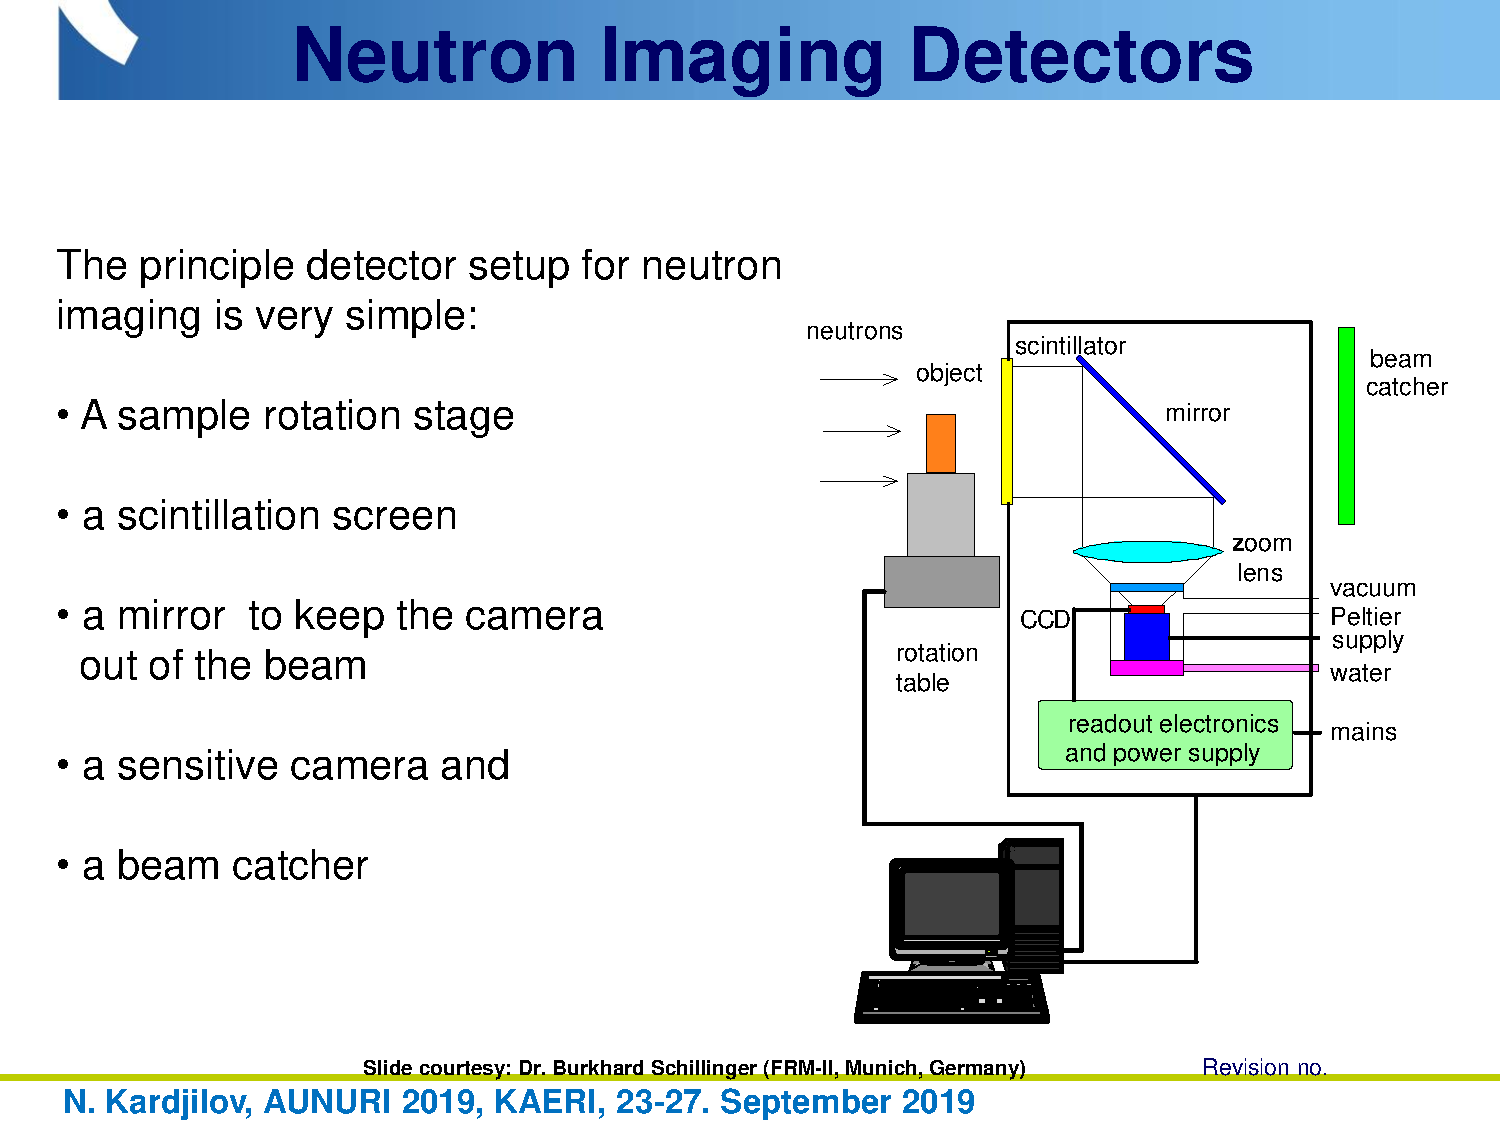
\includepdf{figures/pres4/sl-4.pdf}
\end{frame}
\begin{frame}
  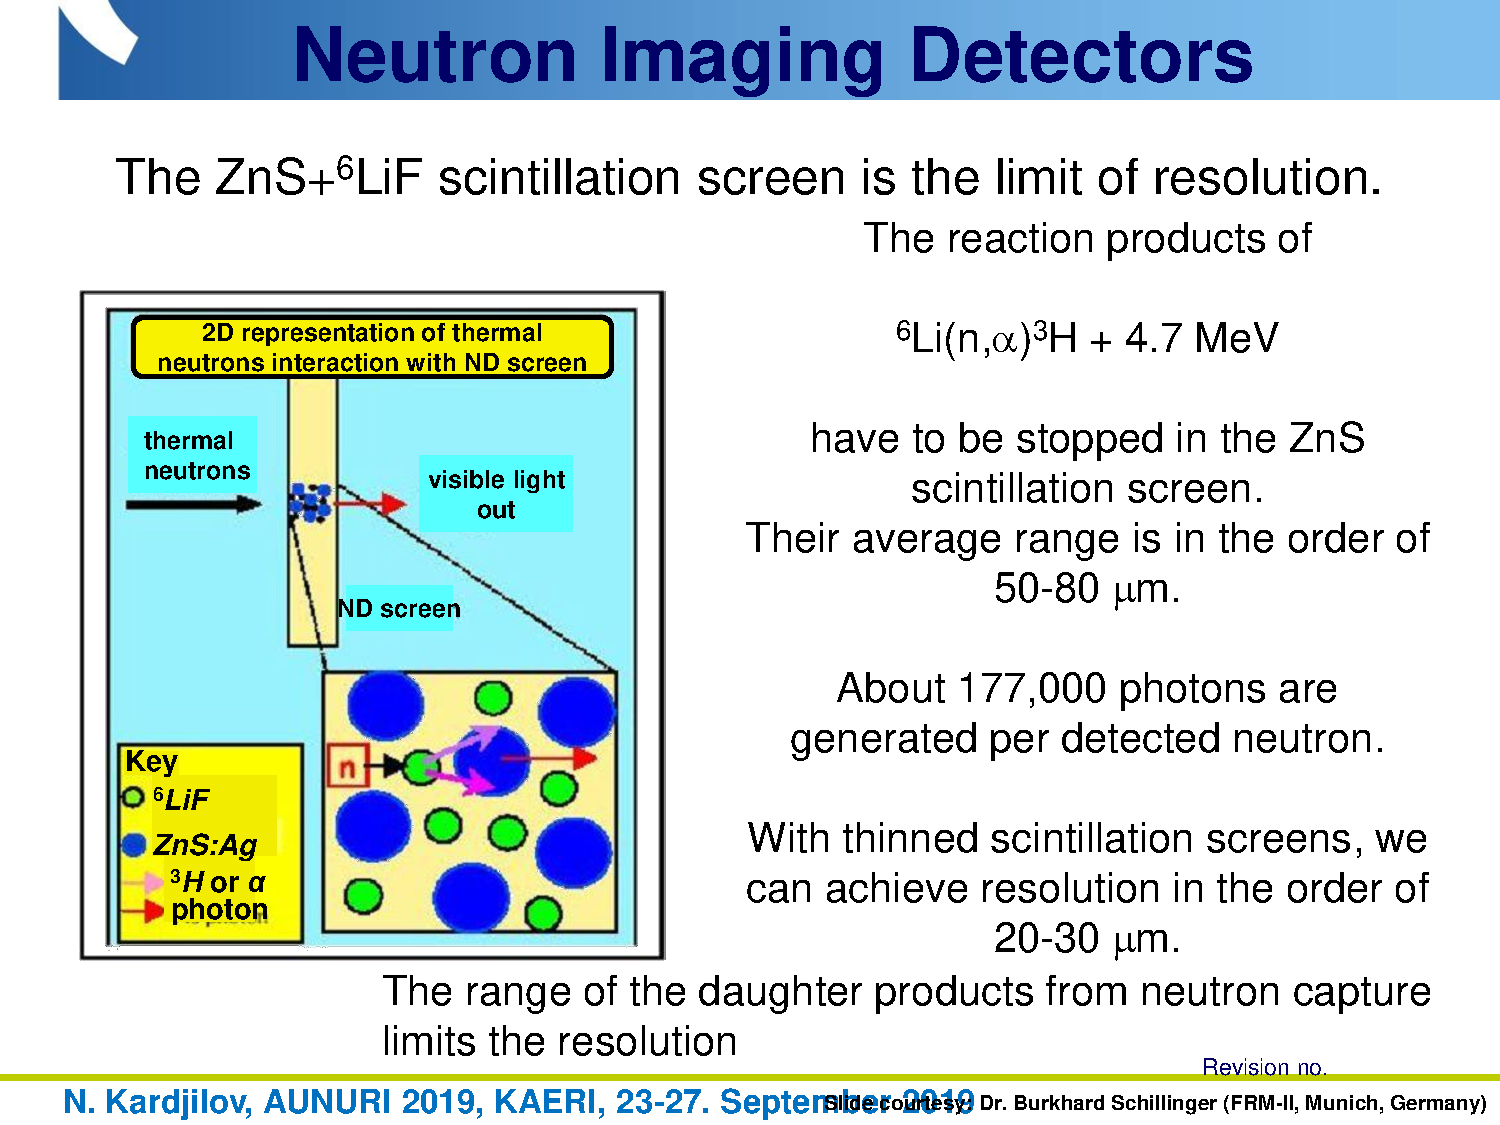
\includepdf{figures/pres4/sl-5.pdf}
\end{frame}
\begin{frame}
  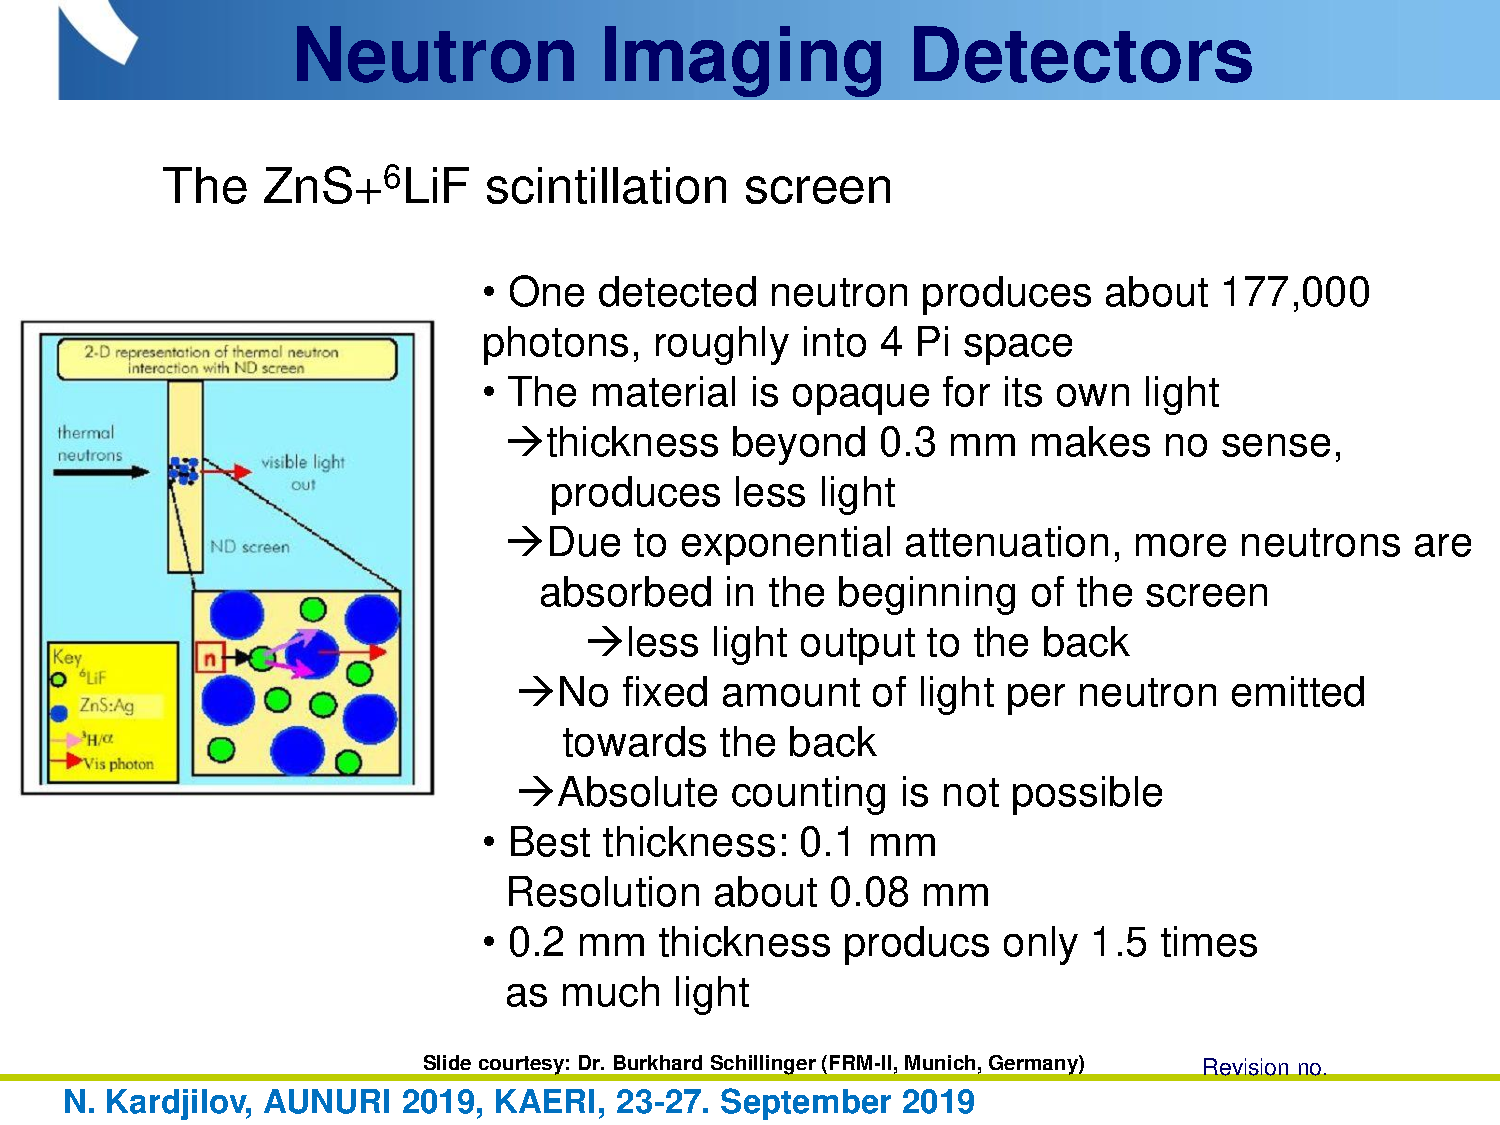
\includepdf{figures/pres4/sl-6.pdf}
\end{frame}
\begin{frame}
  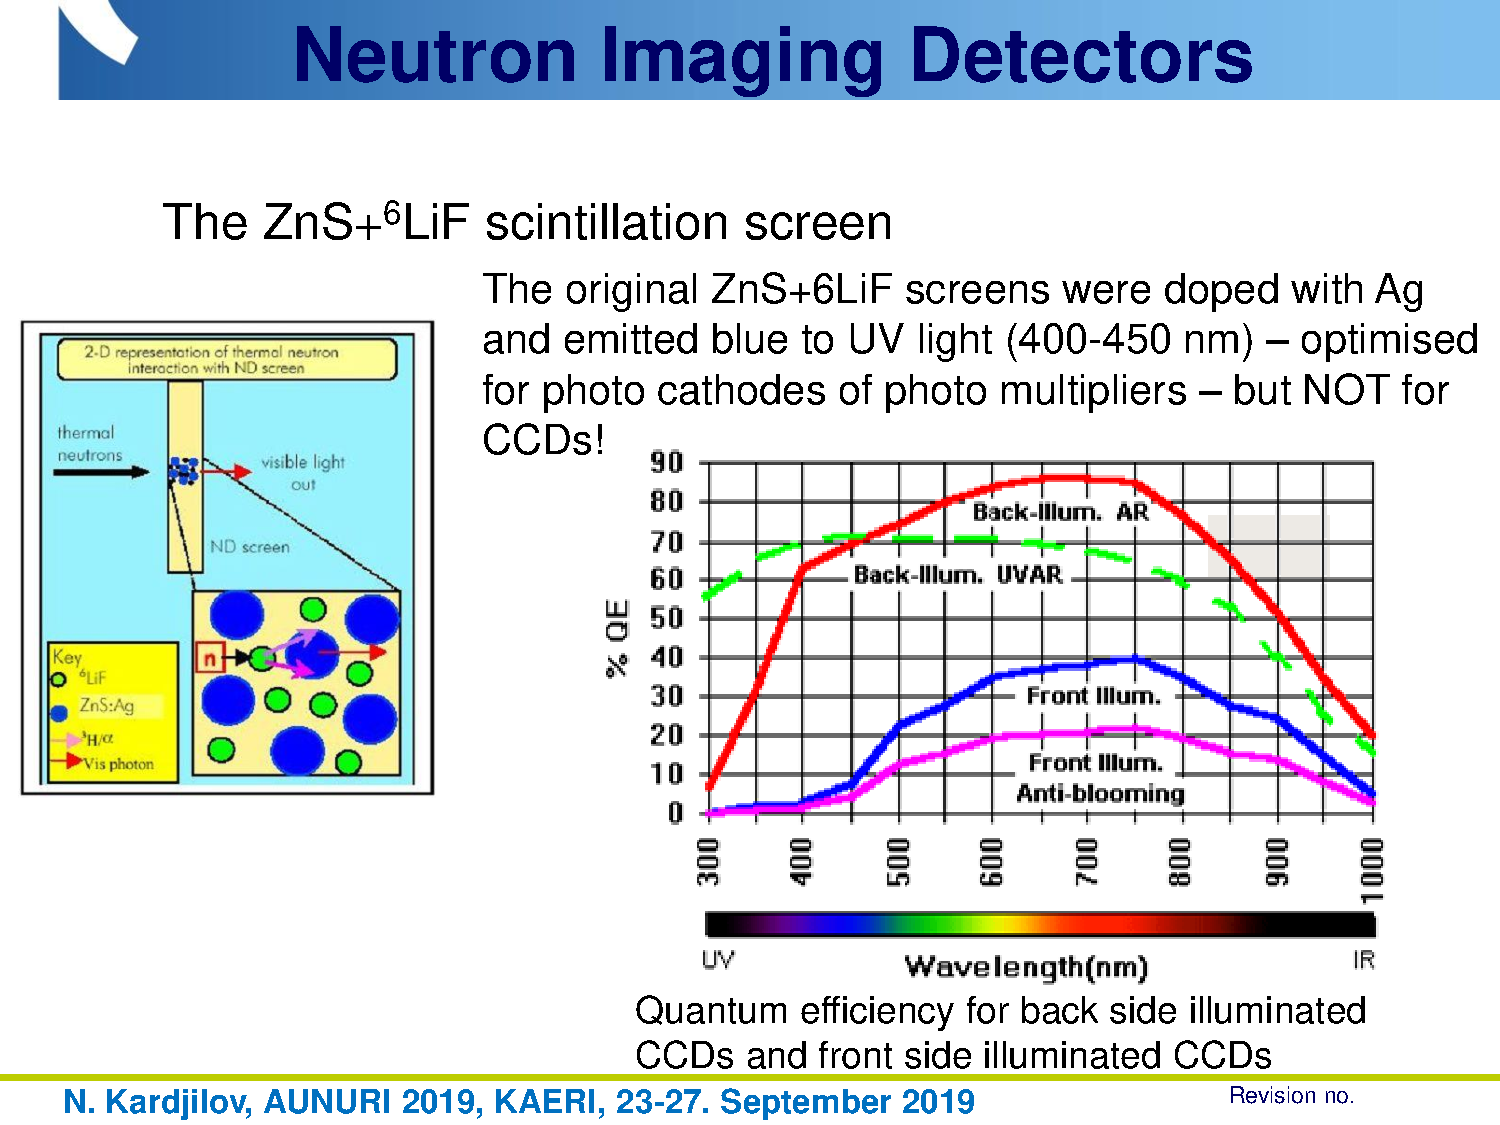
\includepdf{figures/pres4/sl-7.pdf}
\end{frame}
\begin{frame}
  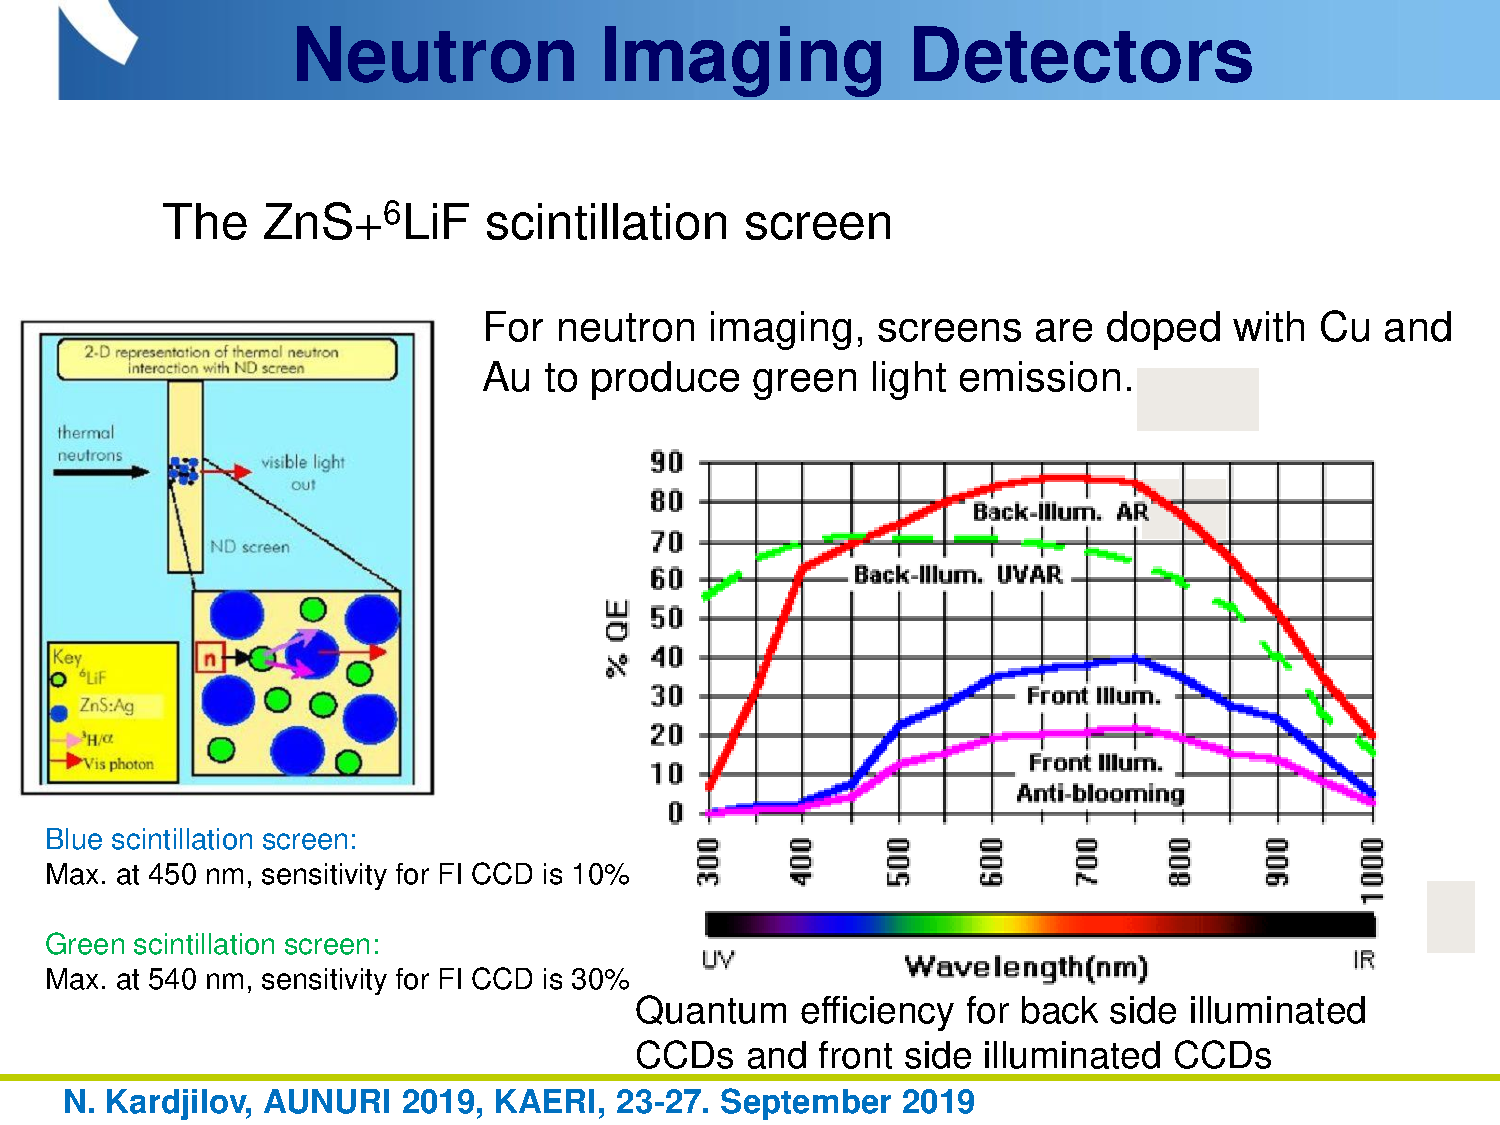
\includepdf{figures/pres4/sl-8.pdf}
\end{frame}
\begin{frame}
  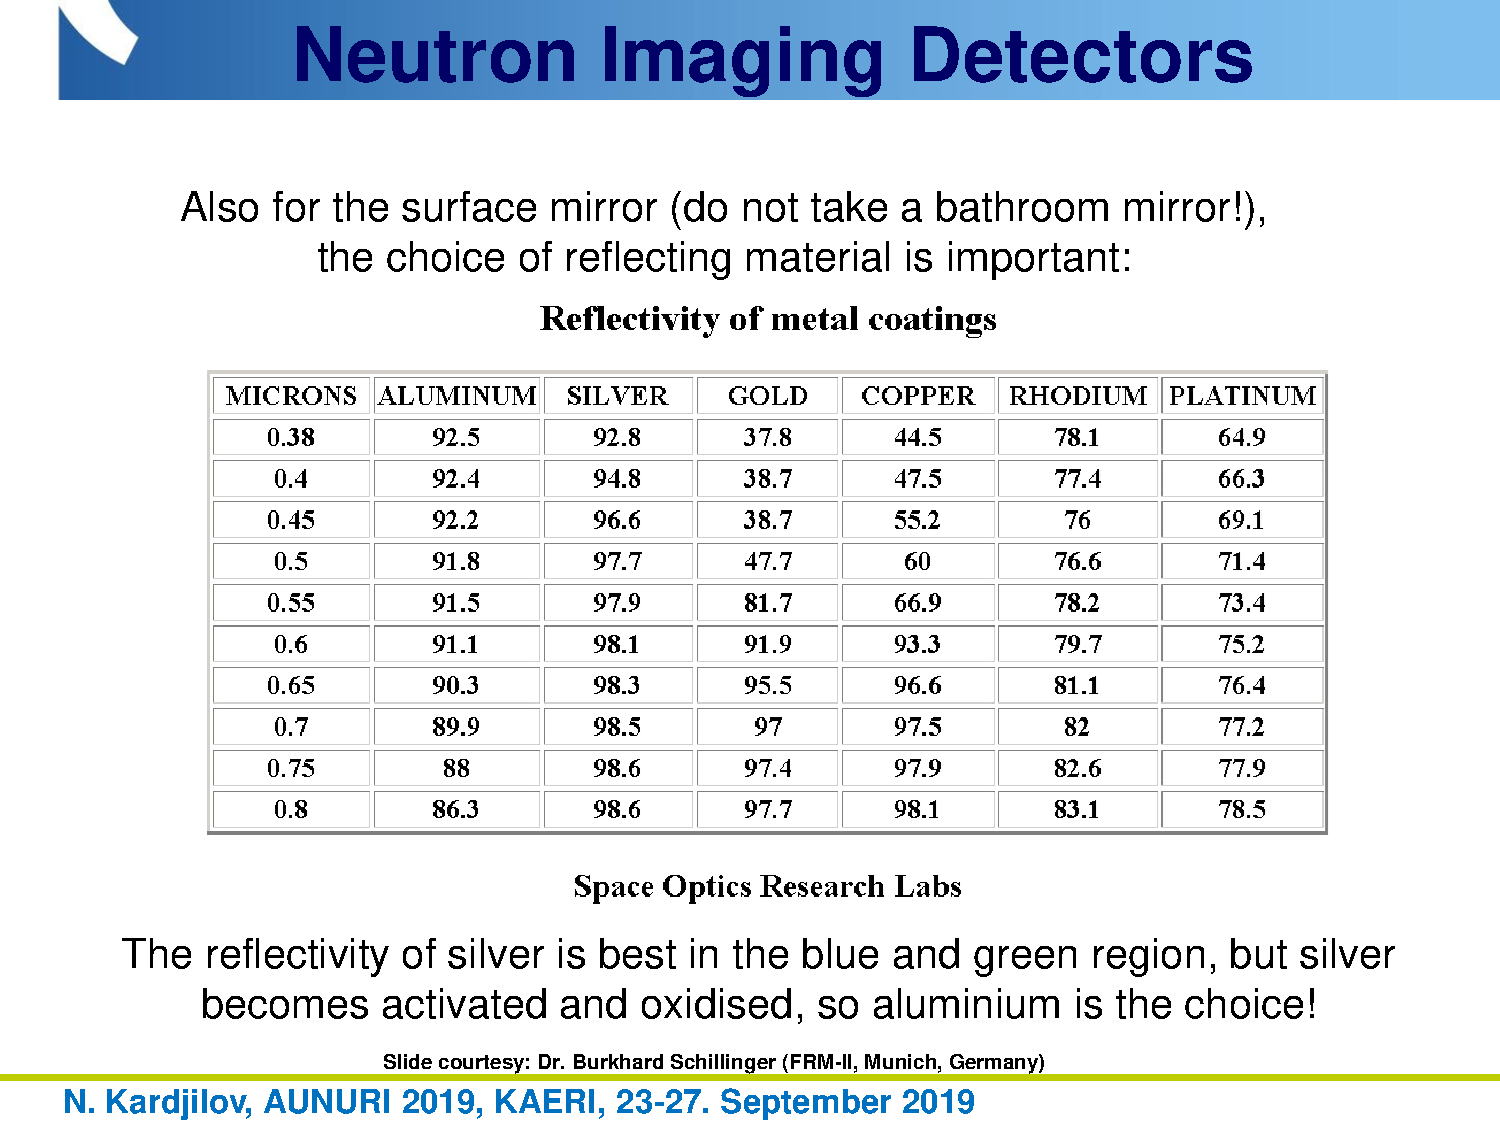
\includepdf{figures/pres4/sl-9.pdf}
\end{frame}
\begin{frame}
  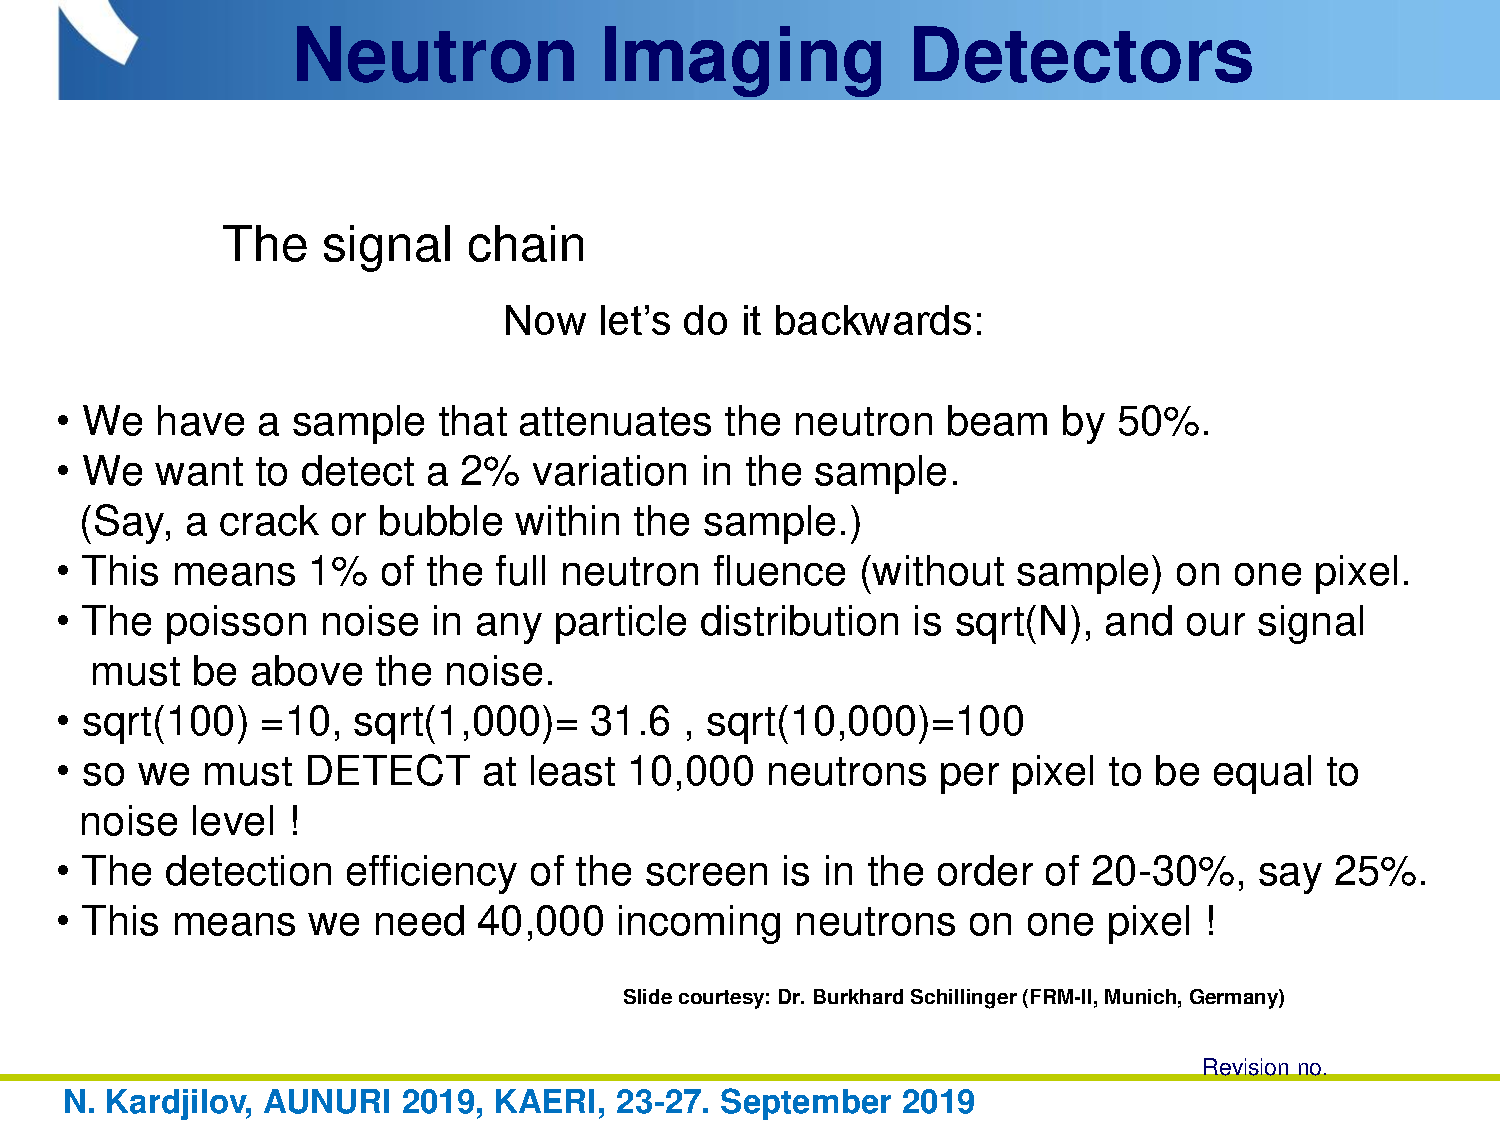
\includepdf{figures/pres4/sl-13.pdf}
\end{frame}
\begin{frame}
  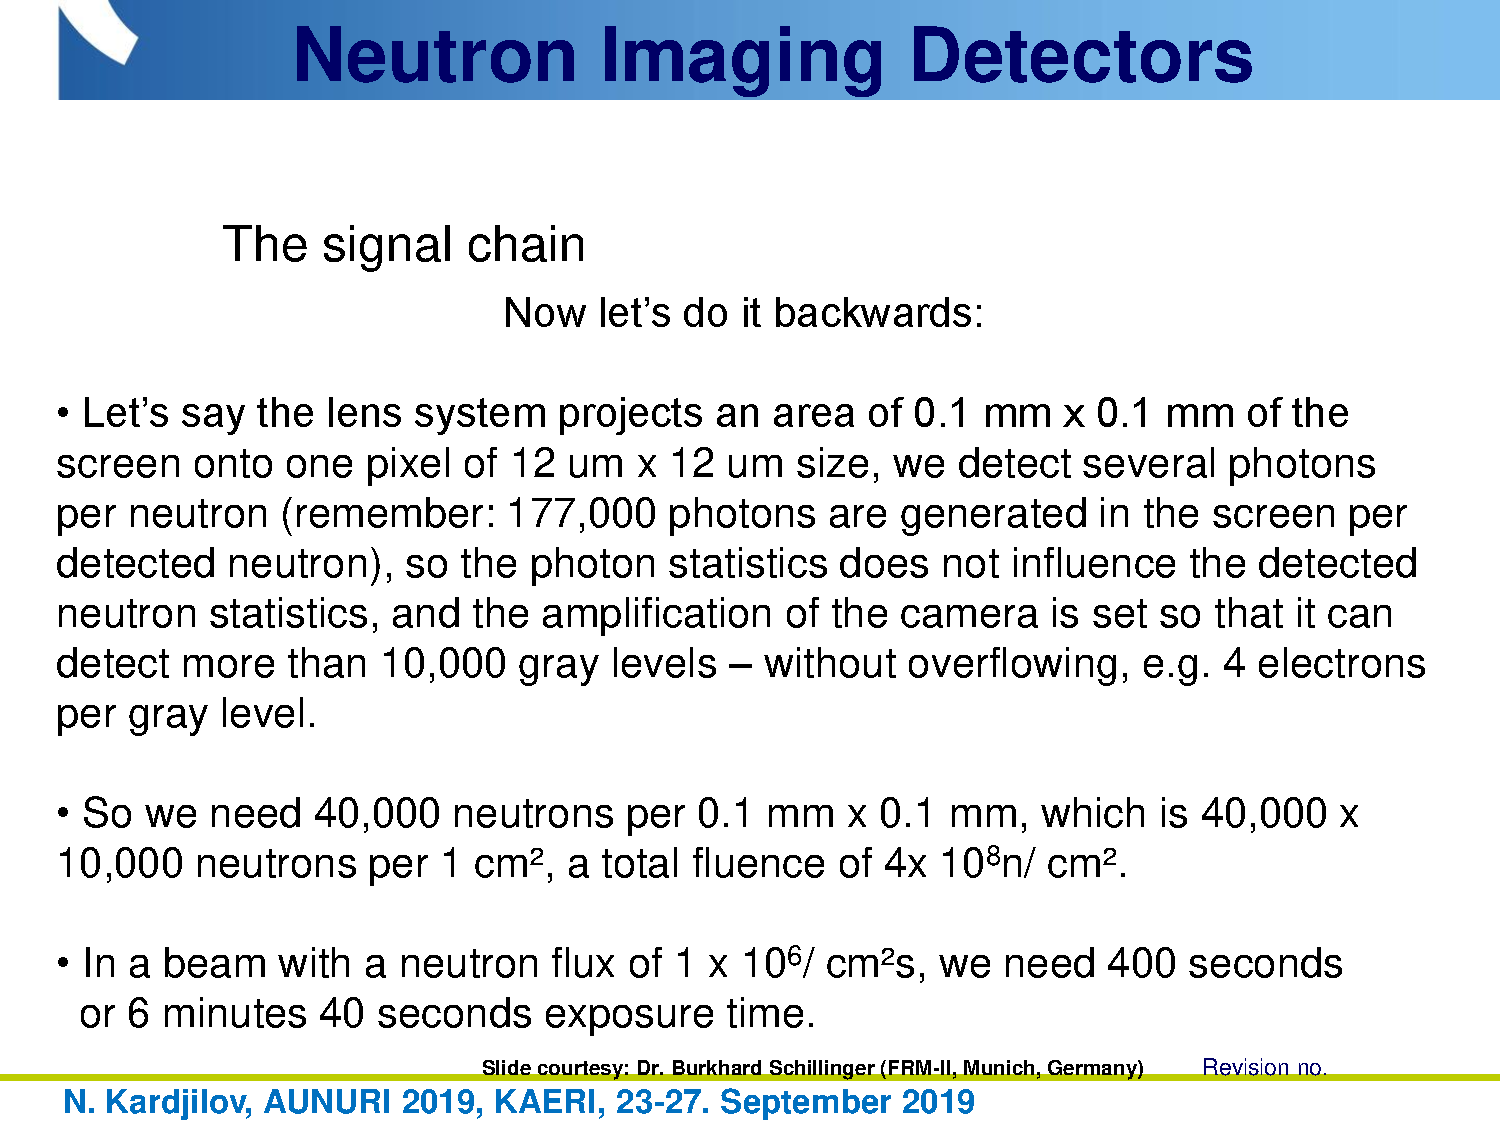
\includepdf{figures/pres4/sl-14.pdf}
\end{frame}
\begin{frame}
  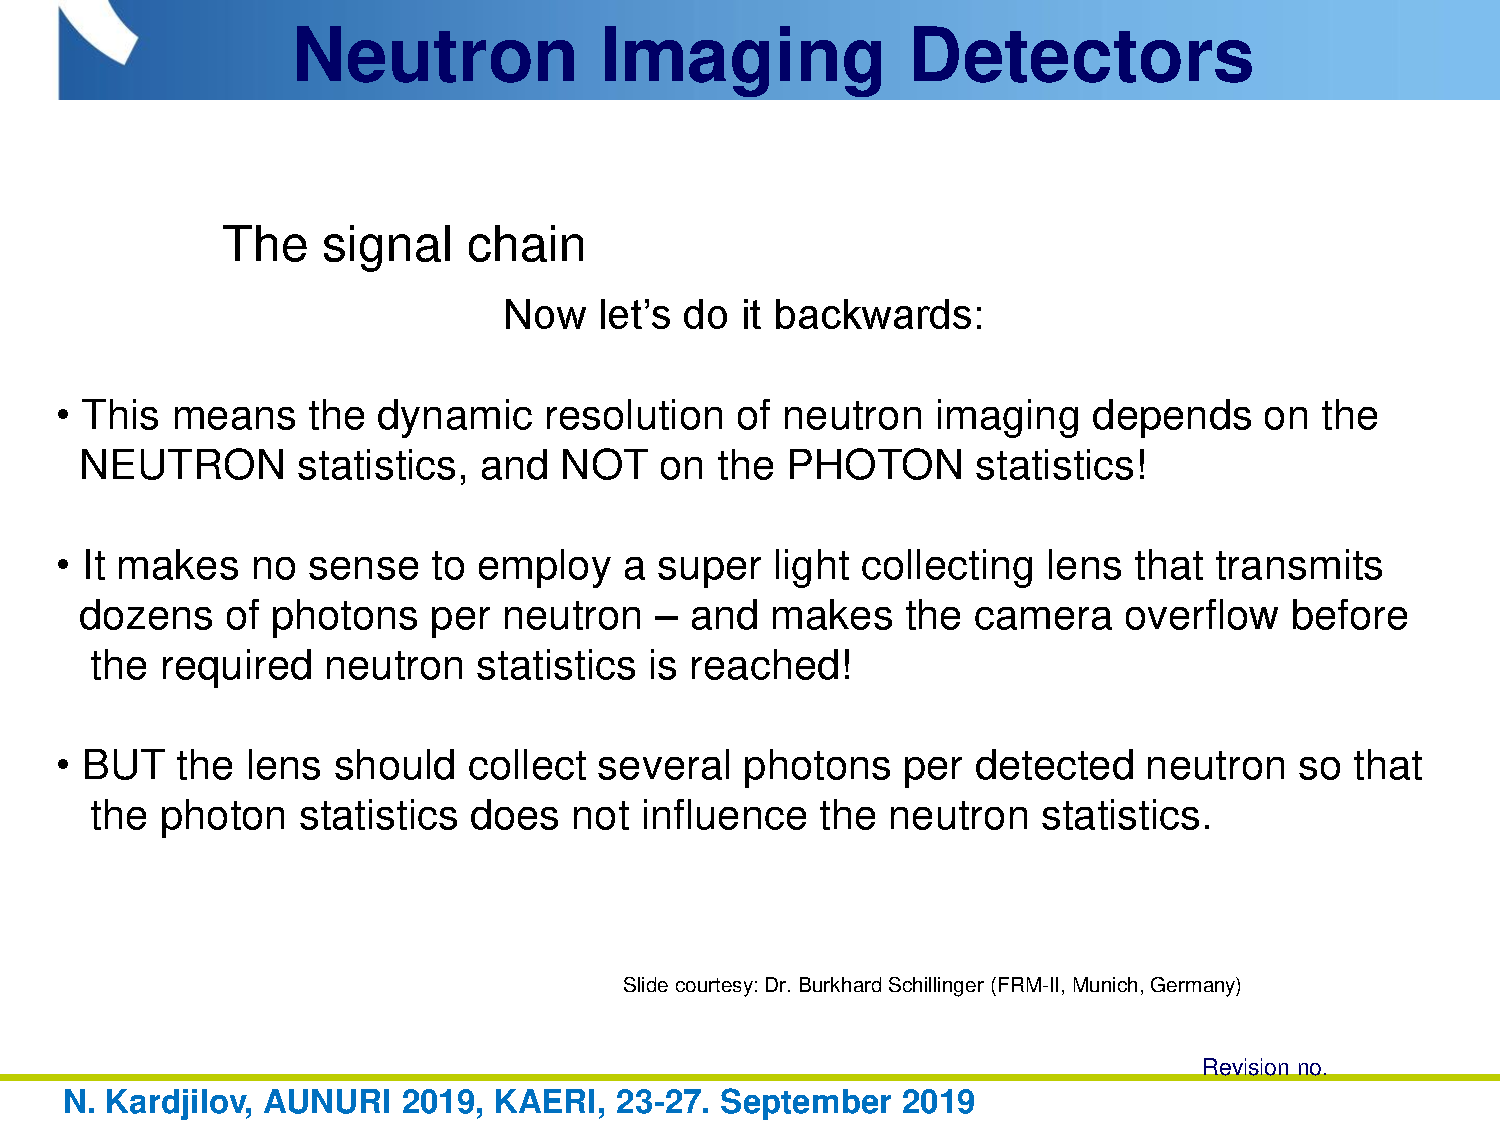
\includepdf{figures/pres4/sl-15.pdf}
\end{frame}
\begin{frame}
  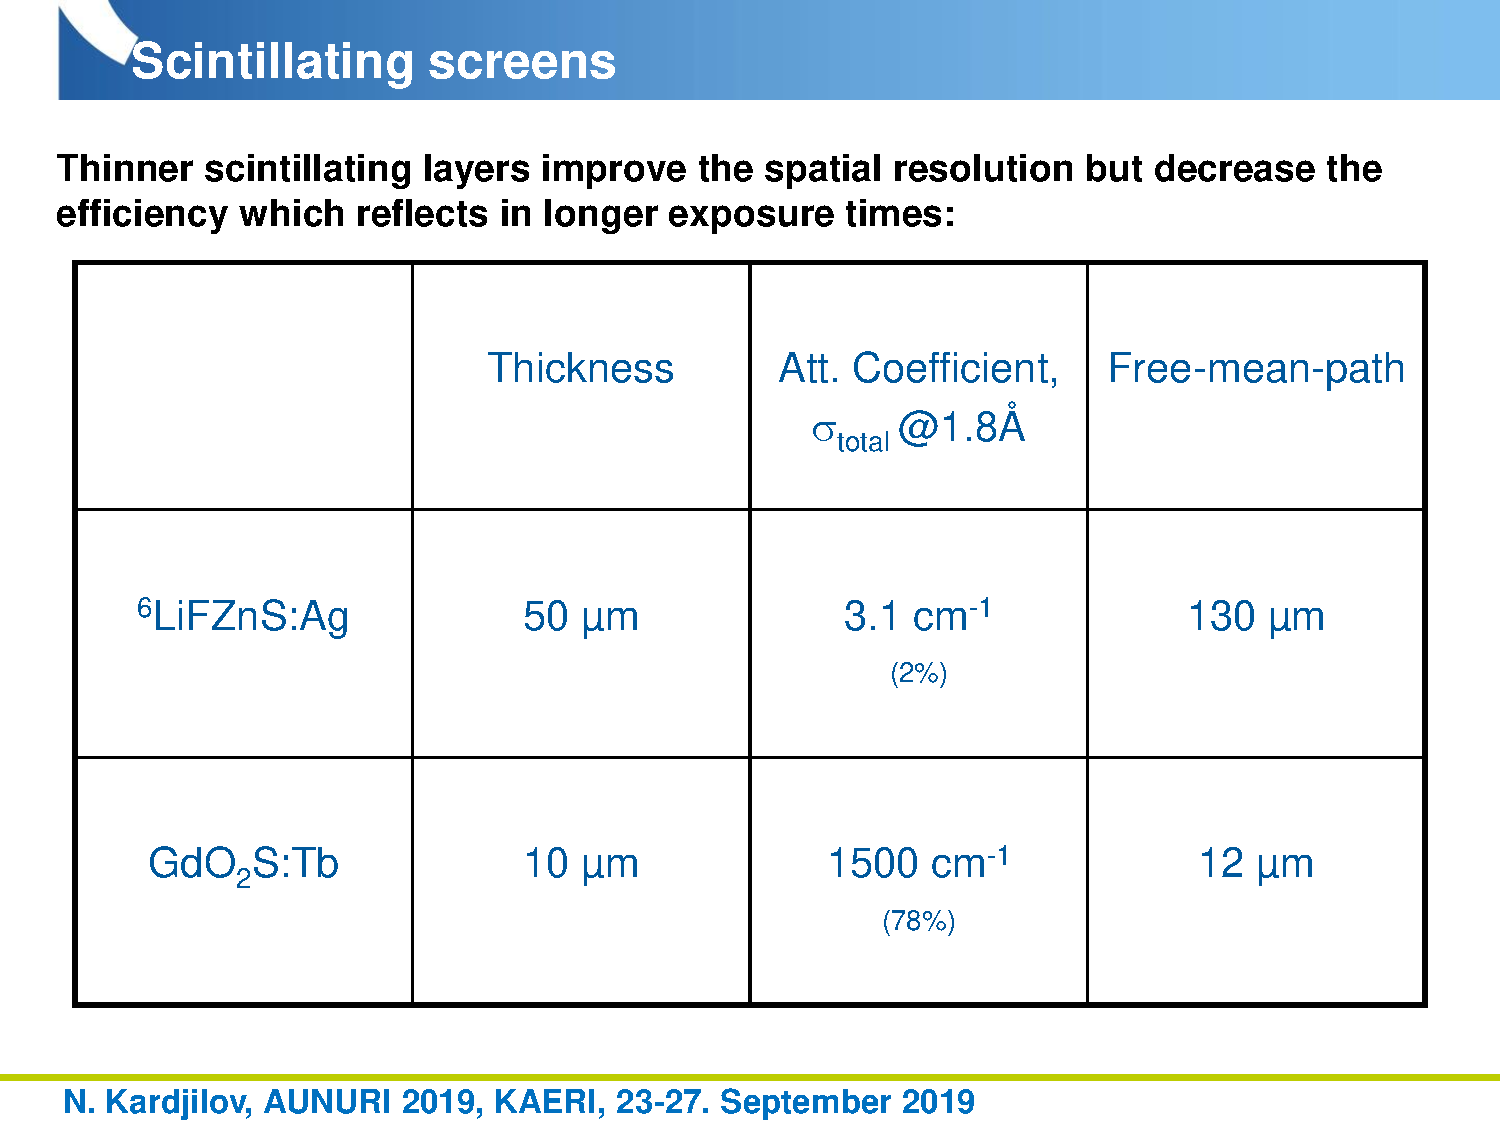
\includepdf{figures/pres4/sl-22.pdf}
\end{frame}
\begin{frame}
  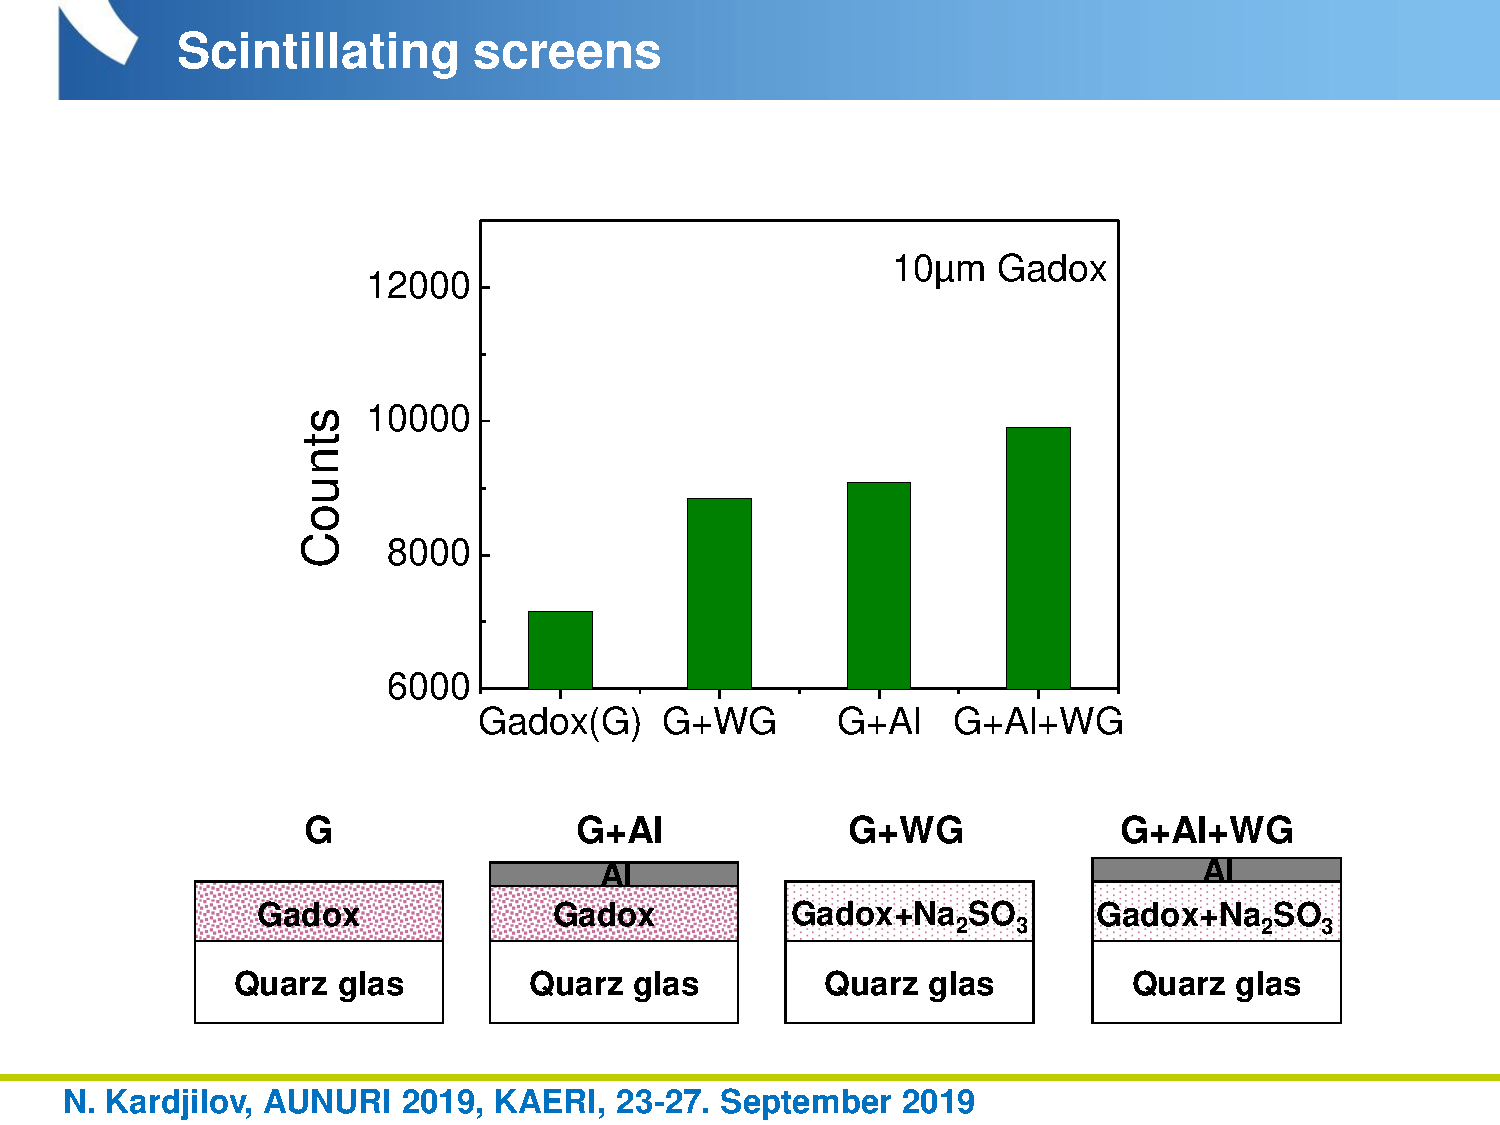
\includepdf{figures/pres4/sl-23.pdf}
\end{frame}
\begin{frame}
  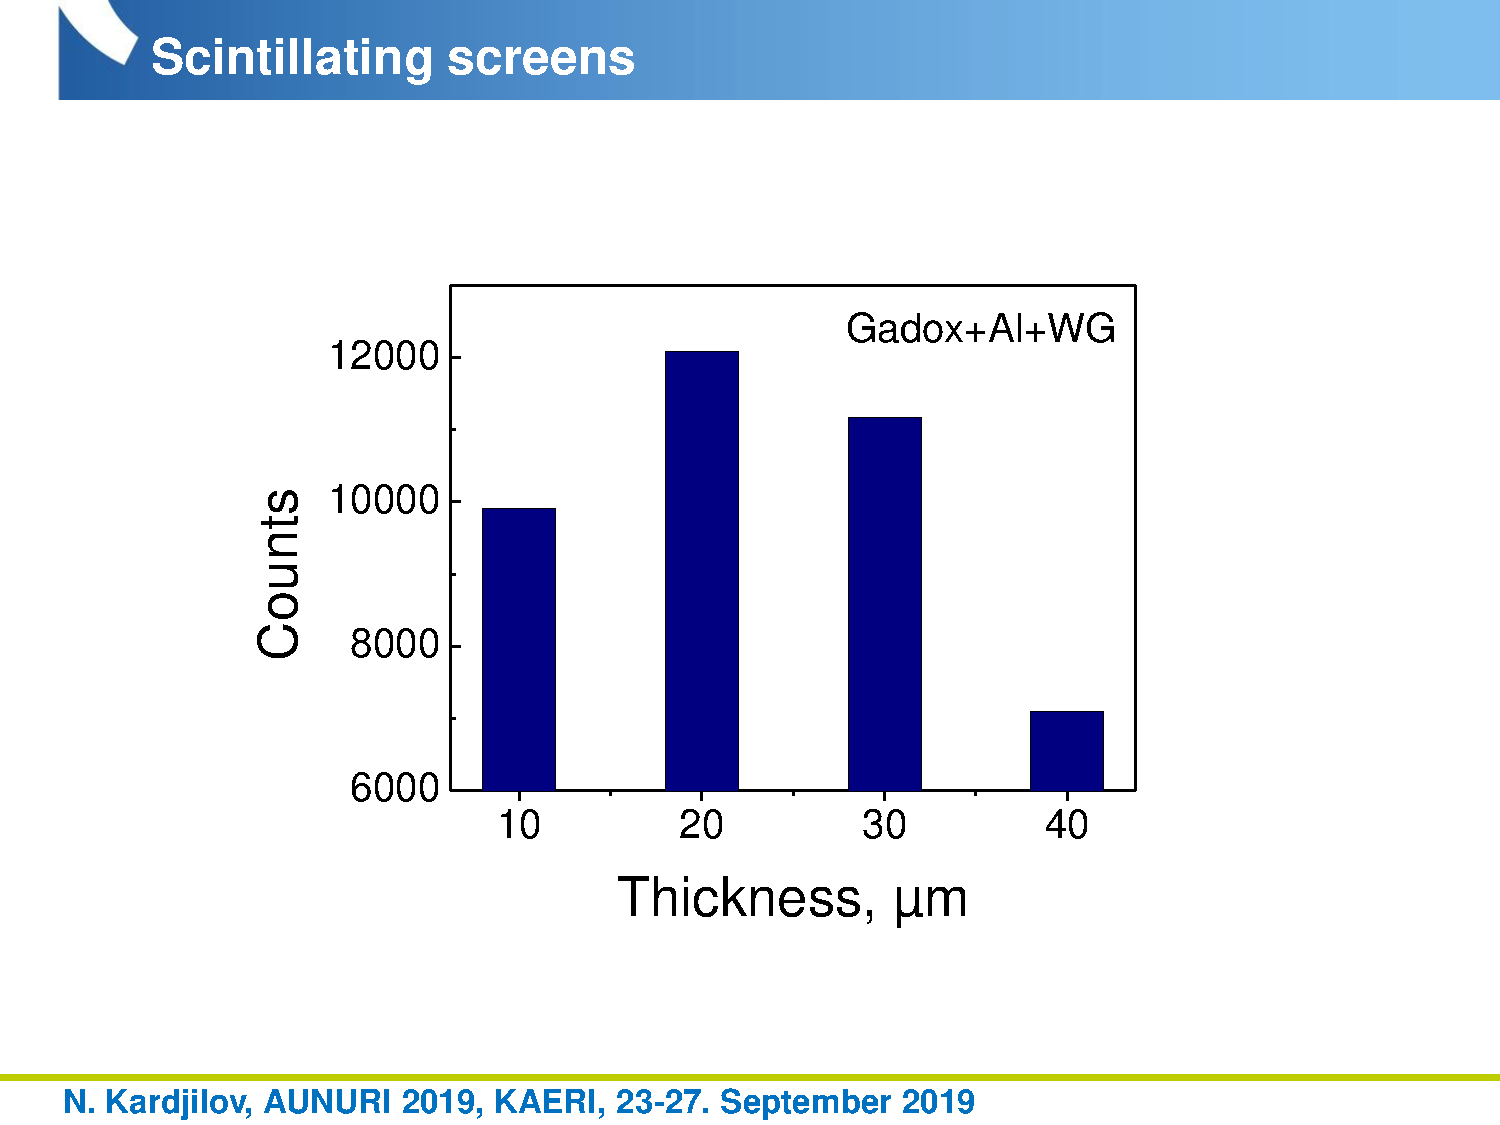
\includepdf{figures/pres4/sl-24.pdf}
\end{frame}

%-------------------------------------------------
\subsection{Simulation of Neutron Imaging Experiments using McStats and MCNP software tools}
%-------------------------------------------------
\begin{frame}
  \frametitle{Apresentações escolhidas}
  \framesubtitle{(5)}
  \begin{center}
    Simulation of Neutron Imaging Experiments using McStats and MCNP software tools\\
    \vspace{2.0cm}
    N. Kardjilov
  \end{center}
\end{frame}

\begin{frame}
  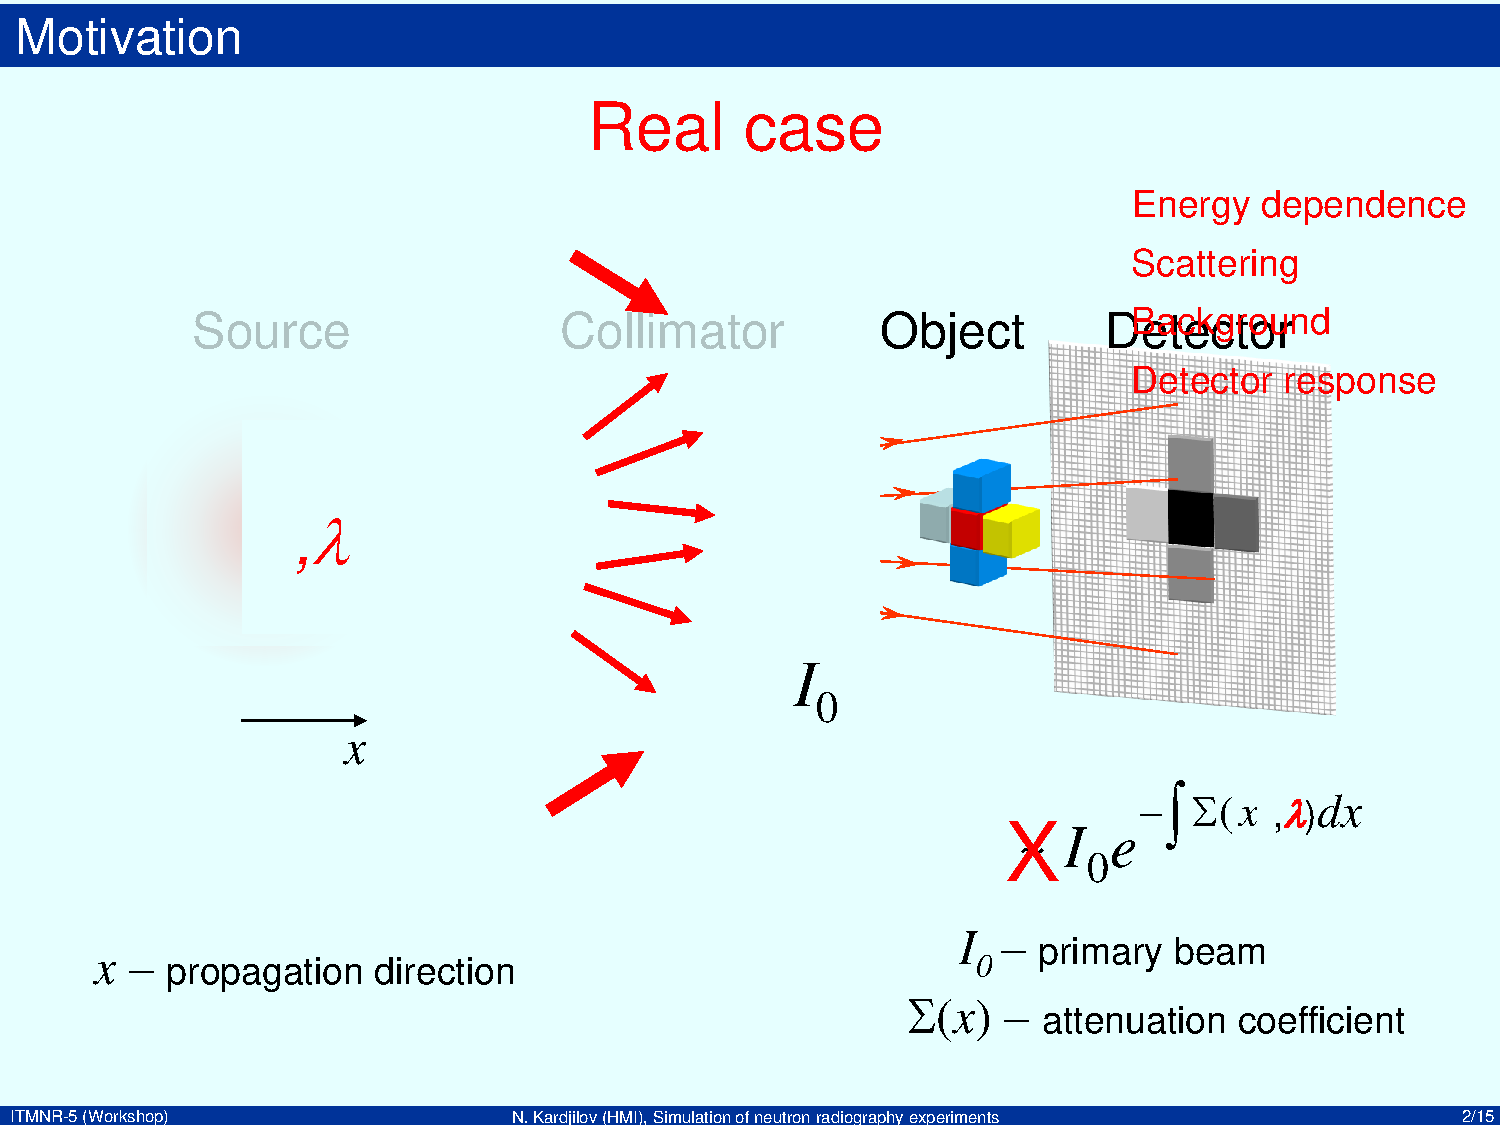
\includepdf{figures/pres5/sl-2.pdf}
\end{frame}
\begin{frame}
  \includepdf{figures/pres5/sl-3.pdf}
\end{frame}
\begin{frame}
  \includepdf{figures/pres5/sl-4.pdf}
\end{frame}
\begin{frame}
  \includepdf{figures/pres5/sl-5.pdf}
\end{frame}
\begin{frame}
  \includepdf{figures/pres5/sl-6.pdf}
\end{frame}
\begin{frame}
  \includepdf{figures/pres5/sl-12.pdf}
\end{frame}
\begin{frame}
  \includepdf{figures/pres5/sl-27.pdf}
\end{frame}
\begin{frame}
  \includepdf{figures/pres5/sl-28.pdf}
\end{frame}
\begin{frame}
  \includepdf{figures/pres5/sl-29.pdf}
\end{frame}
\begin{frame}
  \includepdf{figures/pres5/sl-30.pdf}
\end{frame}
\begin{frame}
  \includepdf{figures/pres5/sl-32.pdf}
\end{frame}
\begin{frame}
  \includepdf{figures/pres5/sl-37.pdf}
\end{frame}
\begin{frame}
  \includepdf{figures/pres5/sl-44.pdf}
\end{frame}
\begin{frame}
  \includepdf{figures/pres5/sl-45.pdf}
\end{frame}

%-------------------------------------------------
\subsection{The IAEA Neutron Imaging e-learning course project}
%-------------------------------------------------
\begin{frame}
  \frametitle{Apresentações escolhidas}
  \framesubtitle{(6)}
  \begin{center}
    The IAEA Neutron Imaging e-learning course project\\
    \vspace{2.0cm}
    N. P. Barradas
  \end{center}
\end{frame}

\begin{frame}
  \includepdf{figures/pres6/sl-1.pdf}
\end{frame}
\begin{frame}
  \includepdf{figures/pres6/sl-3.pdf}
\end{frame}
\begin{frame}
  \includepdf{figures/pres6/sl-11.pdf}
\end{frame}
\begin{frame}
  \includepdf{figures/pres6/sl-12.pdf}
\end{frame}
\begin{frame}
  \includepdf{figures/pres6/sl-13.pdf}
\end{frame}

%-------------------------------------------------
%\subsection{Testing of the e-learning modules}
%-------------------------------------------------
%  \framesubtitle{N. Kardjilov}

%-------------------------------------------------
%\subsection{Outlook and future of Neutron Imaging}
%-------------------------------------------------
%\begin{frame}
%  \frametitle{Apresentações escolhidas}
%  \framesubtitle{(7)}
%  \begin{center}
%    Outlook and future of Neutron Imaging\\
%    \vspace{2.0cm}
%    N. Kardjilov
%  \end{center}
%\end{frame}


\section{Perspectivas de Neutrongrafia no TRIGA IPR-R1}
%-------------------------------------------------
\begin{frame}
  \frametitle{Perspectivas de Neutrongrafia no TRIGA IPR-R1}
  \framesubtitle{Por quê?}
  \begin{enumerate}
  \item Plano DIRETOR 2019-2022: expansão do uso do reator TRIGA;
  \item Estratégia de sobrevivência: maior uso do reator $\rightarrow$ maior importância da instituição;
  \item Neutrongrafia/Imageamento por nêutrons: área de pesquisas/serviços \textbf{ativa} e em relativa expansão;%\pause (demonstrado pelo interesse da AIEA no tema)
  \item Oportunidades de pesquisa, acadêmicas, de serviços e de colaboração institucional.
  \end{enumerate}
%    \vspace{10px}
%  \textbf{Algo aqui?}
%    \begin{itemize}
%    \item bla
%    \end{itemize}
\end{frame}

%-------------------------------------------------
\begin{frame}
  \frametitle{Perspectivas de Neutrongrafia no TRIGA IPR-R1}
  \framesubtitle{Não re-inventar a roda}
  \begin{enumerate}
  \item Há experiência anterior no CDTN com neutrongrafia ainda por filmes\cite{Antonella2002,Antonella2003};
  \item Há experiência \textbf{recente} publicada sobre um sistema completo de imageamento por nêutrons\cite{Wilson2017}; %Colorado School of Mines
  \item Há experiência \textbf{recente} com equipamentos de baixo custo para neutrongrafia e informações disponíveis\cite{Schillinger2019,Turkoglu2013};
    \end{enumerate}
\end{frame}

%-------------------------------------------------
\begin{frame}
  \frametitle{Perspectivas de Neutrongrafia no TRIGA IPR-R1}
  \framesubtitle{Não re-inventar a roda}
  \begin{enumerate}
  \item Há experiência anterior no CDTN com neutrongrafia ainda por filmes\cite{Antonella2002,Antonella2003};
  \item Há experiência \textbf{recente} publicada sobre um sistema completo de imageamento por nêutrons\cite{Wilson2017}; %Colorado School of Mines
  \item Há experiência \textbf{recente} com equipamentos de baixo custo para neutrongrafia e informações disponíveis\cite{Schillinger2019,Turkoglu2013};
    \end{enumerate}
\end{frame}


\section{Conclusões}
%-------------------------------------------------
\begin{frame}[fragile] % Coloca isso no frame que tem verbatim
  \frametitle{Conclusões}
  \begin{itemize}
  \item É possível retomar o imageamento por nêutrons no TRIGA IPR-R1;
  \item Talvez não seja viável $\rightarrow$ mas só é possível sabê-lo através de estudos;
  \item O imageamento por nêutrons pode ser uma nova e sólida utilização do reator com implicações diretas no futuro do CDTN.
  \end{itemize}
\end{frame}

\subsection{Estratégia de curto prazo}
\begin{frame}
  \frametitle{Estratégia de curto prazo}
  \framesubtitle{2020?}
  \begin{enumerate}
  \item Reunir os interessados e fazer o curso de neutrongrafia da AIEA (citado anteriormente);
  \item Estabelecer/Consolidar contatos com instituições com experiência;
  \item Estudos preliminares (cálculos/simulações) com os equipamentos já existentes hoje: obter fluxo com o atual extrator de nêutrons, estudar eventuais mudanças no extrator executáveis na casa, etc.
  \item Contactar eventuais clientes $\rightarrow$ verificar demanda por imageamento por nêutrons.
  \item \alert{Estudar como blindar um feixe de nêutrons vertical!} \pause \cite{Wilson2017}
  \end{enumerate}
\end{frame}

% END SUBSECTION ----------------------------------


%-------------------------------------------------
% FIM
%-------------------------------------------------
\begin{frame}
 \vfill
  \begin{beamercolorbox}[center]{title}
     \Huge{Obrigado!}
  \end{beamercolorbox}
  \vfill
\end{frame}

% ----------------------------
% References
\begin{frame}
    \frametitle{References}
    %\bibliographystyle{apalike}
    \bibliographystyle{apacite}
    \bibliography{aunira2019}
\end{frame}

\end{document}

